% Condensed-out detail derived from the completed chapter/appendix, 2026-10-02.
\documentclass[11pt]{article}
\usepackage[margin=1in]{geometry}
\usepackage{amsmath,booktabs,graphicx,array,placeins,natbib}
\usepackage[hidelinks]{hyperref}
\usepackage{etoolbox,setspace,subcaption}
\BeforeBeginEnvironment{tabular}{\begingroup\setstretch{1}}
\AfterEndEnvironment{tabular}{\endgroup}
\renewcommand{\thesection}{S\arabic{section}}
\renewcommand{\thetable}{S\arabic{table}}
\renewcommand{\thefigure}{S\arabic{figure}}
\renewcommand{\theequation}{S\arabic{equation}}
\makeatletter
\newcommand{\applabel}[2]{\def\@currentlabel{#1}\label{#2}}
\renewcommand{\l@section}{\@dottedtocline{1}{0em}{2.8em}}
\makeatother
\title{Supplementary material: Sampling Design for Spatial Cluster Randomized Trials Under Heterogeneous Incidence}
\author{Andrew Walther, Ashkan Habib, Ross Joseph Simpson, Jr. and Feng-Chang Lin}
\date{October 12, 2026}
\emergencystretch=2em
\begin{document}
\maketitle
\noindent This supplement gives the full methods, results and supporting diagnostics behind the article. It distinguishes the full synthetic grid benchmark, the selected-surface allocation-risk pilot and the completed observed-incidence North Carolina (NC) application. Queen and rook results, planning years and spillover regimes remain separately labeled. The application is a simulation-based design evaluation, not observed intervention efficacy. All data supporting the findings of the simulation study were generated by simulation. The simulation data and R code are available from the authors on request. The North Carolina death-certificate data used in the application are restricted and are not publicly available; only 58-cluster summaries are reported.
\tableofcontents
\clearpage
\section{Detailed simulation methods}\label{detailed-simulation-methods}

\subsection{Spatial structure and outcome
model}\label{spatial-structure-and-outcome-model}

We simulated a \(10\times10\) regular grid of 100 clusters under two
definitions of adjacency. Under queen contiguity, two clusters are
neighbors if they share an edge or a corner; under rook contiguity, they
must share an edge. Queen contiguity is the primary analysis. Rook contiguity is a sensitivity analysis and the
continuity case with earlier work, whose grids used rook neighbors. For
each definition, the binary adjacency matrix was row-standardized to
form the spatial weights matrix \(W\), so that \(WZ\) gives, for each
cluster, the proportion of its neighbors that are treated, and \(WY\)
gives the average outcome among its neighbors. Row-standardization
expresses each cluster's spillover exposure as an average over its own
neighborhood rather than a raw sum, which would otherwise depend on how
many neighbors the cluster has. Within a scenario, the same neighbor
type defines \(W\) in the outcome model, in the Isolation Buffer design,
and in the fitted model.

Cluster-level outcomes \(Y\) were generated from a spatial lag model
with a spillover term, \begin{equation}
Y = (I - \rho W)^{-1}\left[\tau Z + S(Z) + \beta X + \epsilon\right], \qquad \epsilon \sim N(0, \sigma^2 I),
\label{eq:outcome}
\end{equation} where \(Z \in \{0,1\}^{100}\) is the treatment assignment
produced by the design under evaluation, \(\tau\) is the direct
treatment effect of interest, \(S(Z)\) is the spillover term defined in
Equation \ref{eq:spillover}, \(\rho\) is the spatial autoregressive
coefficient governing dependence in the outcome beyond that induced by
treatment and spillover, \(X\) is the baseline incidence covariate with
coefficient \(\beta = 1\), and \(\sigma = 1\). The spatial multiplier
\((I-\rho W)^{-1}\) propagates each cluster's shocks through the network
of neighbors. We tested \(\rho \in \{0, 0.01, 0.20, 0.50\}\). When
\(\rho = 0\) the multiplier is the identity and the model is a linear
regression with independent errors,
\(Y = \tau Z + S(Z) + \beta X + \epsilon\), in which spatial structure
enters only through the spillover term; larger values of \(\rho\) induce
progressively stronger spatial clustering in the outcome.

We evaluated two spillover regimes, \begin{equation}
S(Z) = \gamma\, WZ \quad \text{(both arms)}, \qquad S(Z) = \gamma\, WZ \circ (1 - Z) \quad \text{(control only)},
\label{eq:spillover}
\end{equation} where \(\circ\) denotes the elementwise product. Under
the control-only regime, only untreated clusters respond to the
treatment status of their neighbors, which represents classical
contamination: an untreated cluster's outcome rises with the share of
its neighbors that are treated. Under the both-arms regime, every
cluster responds to its neighbors' treatment regardless of its own
assignment, so neighboring treatment adds to a treated cluster's own
effect. We tested four spillover magnitudes,
\(\gamma \in \{0.5, 0.6, 0.7, 0.8\}\), and five magnitudes of the direct
effect, \(\tau \in \{0.8, 1.0, 1.5, 2.0, 3.0\}\), with \(\tau = 1\) as
the primary scenario throughout.

\subsection{Heterogeneous baseline
incidence}\label{heterogeneous-baseline-incidence}

The earlier small-grid study \citep{walther_spatialcrt_2026} assumed a
spatially uniform baseline outcome risk. Cluster-level health outcomes
typically vary across space, and the designs studied here differ in
whether and how they use that variation. We generated the baseline
incidence covariate \(X\), with values in \((0, 1)\), under three
mechanisms. Under the independent (iid) mechanism, each \(X_i\) is drawn
from a Uniform\((0,1)\) distribution, with no spatial structure. Under
the spatially autocorrelated mechanism,
\(X = \Phi\{(I - \rho_X W_Q)^{-1} u\}\), where \(u \sim N(0, I)\),
\(\Phi\) is the standard normal distribution function applied
elementwise, \(W_Q\) is the queen weights matrix, and
\(\rho_X \in \{0.20, 0.50\}\). Under the Poisson mechanism, a spatially
autocorrelated log-rate surface,
\(\log \lambda = \log(35/100{,}000) + (I - \rho_X W_Q)^{-1} u\) with
\(\rho_X \in \{0.20, 0.50\}\), generates cluster death counts
\(C_i \sim \text{Poisson}(\lambda_i P)\), with an equal population of
\(P = 100{,}000\) in every cluster, so that a cluster at the base rate
expects 35 deaths. The observed rates \(C_i / P\) are then
rank-normalized to \(X_i = (r_i - 0.5)/N\), where \(r_i\) is the rank of
cluster \(i\)'s rate among the \(N = 100\) clusters and tied rates share
their average rank. Ties remain at this population size: the Poisson
surfaces used here have between 60 and 76 distinct values among the 100
clusters. The base rate of 35 per 100,000 was chosen to be
representative of published sudden unexpected death (SUD) incidence: it lies between the SUD
incidence rates that Mirzaei and colleagues estimated for US men (49.3
per 100,000) and women (21.7 per 100,000) aged 20--64, close to their
average \citep{mirzaei_years_2019}. It is not the observed rate of the
county data described in the Application section, which come from a
different source, age range, period, and case definition. The incidence
filters always use the queen weights \(W_Q\), whichever neighbor type
the scenario uses, so the incidence surfaces are identical under rook
and queen contiguity. The iid mechanism and the two strengths of each of
the other two mechanisms give five incidence configurations.

For each configuration we generated \(K = 10\) incidence surfaces,
\(X_1, \dots, X_{10}\), each from its own seed. The same ten surfaces
are used by every scenario in that configuration, across neighbor types,
outcome-model parameters, designs, and values of \(\tau\); the design
draws and the outcome noise are shared more selectively, as described
under Simulation design, resampling, and metrics. Each design is applied
to the surface that generates the outcome: assignments for surface \(k\)
are drawn from \(X_k\), and the outcome and the fitted model for those
assignments use \(X_k\) as well. This assumes that the incidence
observed when a trial is planned is the incidence that drives its
outcome (the matched-surface assumption). The target of each scenario is
performance averaged over incidence surfaces; for example, the mean squared error (MSE) is \(\text{MSE} = E_X E_{Z \mid X} E_\epsilon[(\hat\tau - \tau)^2]\), with
\(X\) drawn from the configuration's generator, \(Z\) from the design
given \(X\), and \(\epsilon \sim N(0, I)\). Bias, coverage, and power
are defined in the same way.

\subsection{Treatment assignment
designs}\label{treatment-assignment-designs}

We implemented eight treatment assignment designs and present six of
them as the primary comparison set in the detailed analysis. The other two, Saturation Quadrants and Balanced Halves, each share the mechanism
of a retained design, and in the comparison of the eight designs and simple random sampling (SRS) at \(\tau = 1\)
neither could be distinguished from its counterpart under either
neighbor type, by the Nemenyi and Holm-adjusted Wilcoxon signed-rank
tests described under Simulation design, resampling, and metrics below,
applied here to all eight designs and SRS. Saturation Quadrants assigns the saturations 20\%, 40\%, 60\%, and 80\% to the four $5\times5$ quadrants of the grid in random order, without reference to incidence. Its retained counterpart, Incidence-Guided Saturation, assigns the higher saturations to the quadrants with higher mean incidence (Table \ref{tab:designs}). On the NC map, both designs use four fixed geographic regions in place of the quadrants. Saturation Quadrants' mean squared error was 0.0900, against 0.0907 for Incidence-Guided Saturation, under
queen contiguity (Nemenyi \(p = 0.99\); Holm-adjusted Wilcoxon
signed-rank \(p = 0.62\)), and 0.0708 against 0.0717 under rook
contiguity (Nemenyi \(p = 1.00\); Wilcoxon \(p = 1.00\)). We retain one
representative of the saturation mechanism, Incidence-Guided Saturation. Saturation Quadrants had the marginally lower mean under both
neighbor types and the better average rank in this
comparison (2.394 against 2.700 under queen contiguity and 2.587 against
2.650 under rook contiguity), so this choice does not rest on performance. The two saturation designs performed similarly, so incidence guidance matches the accuracy of Saturation Quadrants while directing the highest treatment saturations to the quadrants or regions with the highest incidence. How much treatment it redirects depends on how much incidence differs between regions (Section \ref{app:nc-ext}). The accuracy advantage of both designs over SRS, which arises under control-only spillover (see SRS benchmark and allocation-specific risk), comes from the saturation structure they share.
Balanced Halves divides clusters into two halves by incidence rank and
treats 25 at random in each. Its mean squared error was 0.1299, against
0.1308 for Balanced Quartiles, under queen contiguity (Nemenyi
\(p = 1.00\); Wilcoxon \(p = 1.00\)), and 0.0842 against 0.0837 under
rook contiguity (Nemenyi \(p = 1.00\); Wilcoxon \(p = 1.00\)). The two
designs differ only in how finely they stratify on incidence, and we
retain the finer, four-stratum version. Balanced Halves had the
marginally lower mean and the better average rank under queen contiguity
(3.831 against 3.906), and Balanced Quartiles had both under rook
contiguity (3.369 against 3.569), so this choice does not rest on
performance either. Both related variants, and the full eight-design
comparison, are reported in Section \ref{app:eight-design}.

Table \ref{tab:designs} describes the six retained designs, and Figure
\ref{fig:design-samples} shows one assignment from each, and from SRS, on a single
illustrative incidence surface. Checkerboard is the strict
block-stratified allocation of the earlier small-grid study, in which no
two rook neighbors share an arm. The earlier small-grid study's Block
Stratified Sampling design also admitted relaxed allocations on its
\(3\times3\) grid, where the arms cannot be balanced; on its
\(2\times4\) and \(3\times4\) grids, as on the \(10\times10\) grid here,
the strict allocations are the two checkerboard patterns. We use the two
names interchangeably for this allocation and use Checkerboard in the
rest of the detailed analysis. Checkerboard is the only deterministic
design: it gives the same assignment in every draw, although each of its
fits still receives its own outcome noise. Every other design was drawn
independently 25 times for each incidence surface. Designs that rank
clusters by incidence break ties at random, afresh for each draw. High
Incidence Focus is random only through that tie-breaking; under the iid
and spatial mechanisms incidence values are distinct, so it gives the
same assignment in all 25 draws on a surface, and its assignment changes
only from one surface to the next. Isolation Buffer builds its
assignment from the neighbor type of the scenario, and it treats 38
clusters on average under rook contiguity and 21 under queen contiguity.
Every other design treats exactly 50.

\begin{table}[!htb]

\small
\centering

\caption{The six treatment assignment designs compared in the detailed analysis, ordered by mean squared error under queen contiguity at $\tau = 1$, pooled over the five incidence configurations (Table \ref{tab:performance}). A cluster's incidence rank is its rank by the baseline incidence surface $X_k$, with ties broken at random in every draw. Clusters treated is the number of clusters treated per assignment; for Isolation Buffer, which depends on the neighbor type, it is the mean over its assignments under each neighbor type.}
\label{tab:designs}

\begin{tabular}{p{3.4cm}p{6.4cm}p{2.0cm}p{2.3cm}}

\toprule
Design & Assignment rule & Clusters treated & Deterministic \\

\midrule
Incidence-Guided Saturation & The grid is divided into its four $5\times5$ coordinate quadrants. Quadrants are ranked by mean incidence and given saturations of 80\%, 60\%, 40\%, and 20\% from highest to lowest mean; within each quadrant, that share of its 25 clusters is treated at random & 50 & No \\
Balanced Quartiles & Clusters are divided by incidence rank into four strata of 25. Twelve clusters are treated at random in each stratum, and one more in each of two randomly chosen strata & 50 & No \\
Isolation Buffer & Clusters are treated one at a time, each chosen at random from those that are neither treated nor adjacent to a treated cluster, until none remain (a greedy random maximal independent set); no two treated clusters are neighbors & \raggedright 38 rook, 21 queen (mean) & No \\
High Incidence Focus & The 50 clusters with the highest incidence rank are treated & 50 & No \\
2$\times$2 Blocking & The grid is divided into 25 non-overlapping 2$\times$2 blocks; two of the four clusters in each block are treated at random & 50 & No \\
Checkerboard (strict Block Stratified Sampling allocation in the earlier small-grid study) & Clusters whose grid coordinates $(x, y)$ have an odd sum $x + y$ are treated, so treatment alternates from cluster to cluster; under rook contiguity every neighbor of a treated cluster is a control, and every neighbor of a control is treated & 50 & Yes \\

\bottomrule

\end{tabular}

\end{table}

\begin{figure}[!htb]

\centering
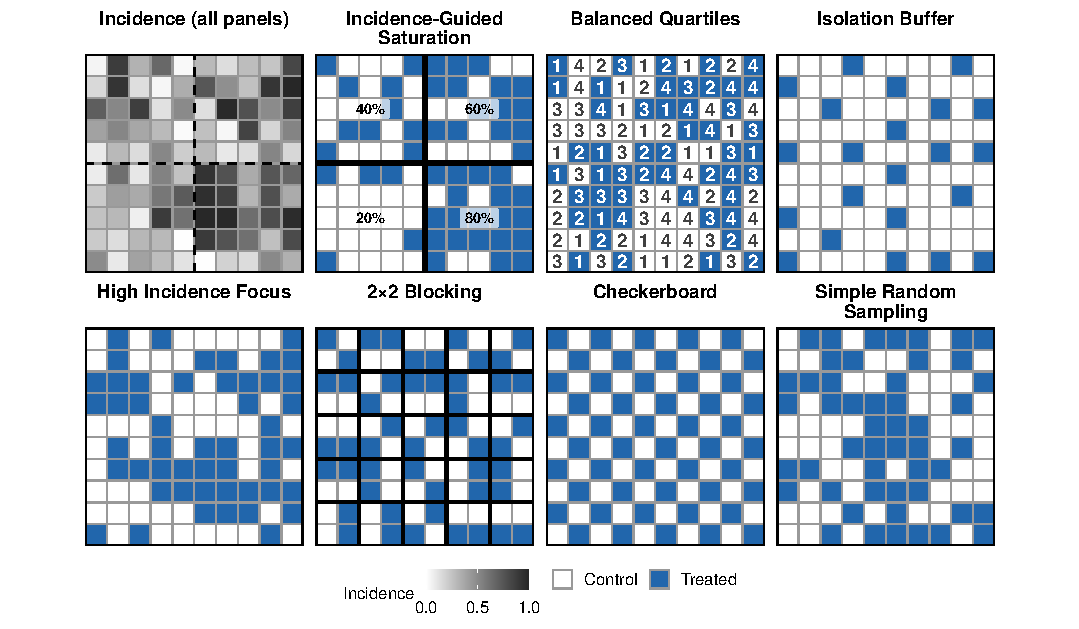
\includegraphics[width=0.85\linewidth]{../figures/design_assignments_panels.pdf}

\caption{One example assignment from each of the six designs and SRS on the $10\times10$ grid, with the designs in the order of Table \ref{tab:designs} followed by SRS. Every example uses the illustrative incidence surface in the first panel (darker is higher; dashed lines mark the quadrants), a spatially autocorrelated surface with $\rho_X = 0.5$ generated with a fixed seed; it is not one of the simulation's incidence surfaces. Blue clusters are treated and white clusters are controls. Lines mark the $2\times2$ blocks and the quadrants, numbers in the Balanced Quartiles panel give each cluster's incidence quartile, and percentages in the Incidence-Guided Saturation panel give each quadrant's treated share. Isolation Buffer is shown under queen contiguity.}
\label{fig:design-samples}

\end{figure}

\subsection{Estimation}\label{estimation}

We estimated \(\tau\) with two maximum likelihood spatial lag models,
both fit to every simulated outcome and both including an intercept. The
primary, oracle model has the spatial lag \(\rho WY\) and the covariates
\(Z\), \(\text{Spill} = S(Z)\), and \(X_k\), so it matches the outcome
model in Equation \ref{eq:outcome}, including the true regime-specific
spillover covariate from Equation \ref{eq:spillover}. The oracle model
assumes that the analyst knows the form of the spillover mechanism and
has the exact exposure term, so its results are a best case for each
design; we return to this assumption as a limitation. The non-oracle
model, a sensitivity analysis, has the covariates \(Z\) and \(X_k\) only
and omits the spillover term. Both models are fit to the same outcomes.

We fit both models with our own implementation of the maximum likelihood
estimator of the spatial lag model \citep{bivand_comparing_2015}, the
same estimator that the \texttt{lagsarlm} function of the R package
\texttt{spatialreg} computes with \texttt{method\ =\ "eigen"}. It
maximizes the concentrated log-likelihood over \(\rho\), computing the
log-determinant from the eigenvalues of \(W\)
\citep{ord_estimation_1975}, estimates the remaining coefficients by
least squares given \(\hat\rho\), and computes standard errors from the
analytic information matrix. On 5,120 validation fits it agreed with
\texttt{lagsarlm} to within \(9.7\times10^{-8}\) in \(\hat\tau\) and to
a relative difference of \(1.1\times10^{-8}\) in its standard error, at
roughly 1\% of the computing time; we also refit a 1\% sample of the
full simulation with \texttt{lagsarlm} itself as a check. Confidence intervals are 95\% intervals with a $t$ reference distribution and a degrees-of-freedom-corrected standard error, $\hat\tau \pm t_{0.975,\,N-p}\,\widehat{\text{SE}}\sqrt{N/(N-p)}$, where $\widehat{\text{SE}}$ is the estimated standard error, $N = 100$ is the number of clusters and $p$ is the number of regression coefficients plus $\rho$ (5 for the oracle model; 4 for the non-oracle model and for rook Checkerboard, whose aliased spillover column is dropped). The application uses the same interval. The 95\% Wald interval, $\hat\tau \pm 1.96\,\widehat{\text{SE}}$, covered about one percentage point less for every design.

Checkerboard illustrates why interspersion alone cannot guarantee
precision. Under rook contiguity on the rectangular grid, \(WZ=1-Z\), so
treatment and spillover cannot be separately identified; the fitted
coefficient on treatment estimates \(\tau-\gamma\). Under queen
contiguity, treatment is identified but control-only spillover is weakly
separated from treatment. We retain Checkerboard in the main design
comparison and flag aliased estimates. Exact matrix identities, boundary
information and the rare Isolation Buffer aliases are detailed in
Section \ref{app:technical}. These diagnostics concern the models
implemented here.

\subsection{Simulation design, resampling, and
metrics}\label{simulation-design-resampling-and-metrics}

The full simulation crossed five values of \(\tau\), five incidence
configurations, two neighbor types, four values of \(\rho\), four values
of \(\gamma\), two spillover regimes, and eight designs, for
\(5 \times 5 \times 2 \times 4 \times 4 \times 2 \times 8 = 12{,}800\)
scenarios, of which the six designs reported in the detailed analysis
account for 9,600. We call a combination of incidence configuration,
neighbor type, \(\rho\), \(\gamma\), and spillover regime a block; there
are \(5 \times 2 \times 4 \times 4 \times 2 = 320\) blocks, 160 for each
neighbor type. At the primary scenario, \(\tau = 1\), the six designs
give 1,920 scenarios, and every block contains all six.

Within each scenario, we drew \(J = 25\) assignments from each of the
\(K = 10\) incidence surfaces, for 250 fits per scenario, and gave every
fit its own noise vector, so that fit \((k, j)\) has outcome
\(Y_{kj} = (I - \rho W)^{-1}[\tau Z_{kj} + S(Z_{kj}) + \beta X_k + \epsilon_{kj}]\).
Checkerboard's 250 fits share one assignment but have 250 distinct noise
vectors. Given a surface, its 25 pairs of assignment and noise are
independent, and the ten surfaces are independent of one another, so the
surface is the primary sampling unit. Each estimator was fit 3.2 million
times. SRS was subsequently run with the same matched surfaces, noise
keys and 250-fit structure, bringing the complete benchmark to 14,400
scenarios and 3.6 million fits per estimator; the original eight-design
results were unchanged. SRS assigns exactly 50 of the 100 clusters to
treatment by complete randomization, ignoring incidence and geography.

Every random draw was seeded from a hash of a key that names the draw:
the configuration and surface index for an incidence surface; the block,
surface, and design for a set of 25 assignments; and the block for the
noise. Each draw therefore depends only on its key, and the results are
identical whether scenarios are run sequentially, in parallel, or in any
order. The keys also give common random numbers. Within a block, all
designs share the same noise vectors and incidence surfaces; the five
values of \(\tau\) reuse the same assignments and noise; and the oracle
and non-oracle models are fit to the same outcomes. Assignments and
noise are independent across blocks, but blocks within an incidence
configuration share its ten surfaces.

For each scenario and estimator, we computed five metrics over the valid
fits, those with a finite estimate and standard error: bias, the mean of
\(\hat\tau - \tau\); the standard deviation (SD) of \(\hat\tau\); mean
squared error, \(\text{MSE} = \text{mean}\{(\hat\tau - \tau)^2\}\);
coverage, the fraction of fits with \(L \le \tau \le U\), where \(L\) and \(U\) are the limits of the 95\% interval defined above; and power, the
fraction of fits with \(L > 0\), a one-sided test of \(\tau = 0\) at
level 0.025. For both estimators, every one of the 250 fits in every
scenario was valid, and the fitting routine raised no warning other than
the aliasing flags described above.

Because each metric is estimated from a finite number of simulated datasets, it carries simulation (Monte Carlo) error; its Monte Carlo standard error
measures this uncertainty and shrinks as more datasets are simulated.
Monte Carlo standard errors come from the surface-level metrics. For a
metric \(m\), we computed \(m_k\) on the 25 fits from surface \(k\) and
set \(\text{SE}(m) = \text{sd}(m_1, \dots, m_{10})/\sqrt{10}\), with
intervals \(m \pm t_{0.975,\,9}\,\text{SE}(m)\). A difference between
two designs is paired at the surface level: its standard error is that
of \(m_{d,k} - m_{d',k}\) over \(k\). For a metric pooled over the five
incidence configurations, we apply the same formula to the 50
configuration-by-surface means, each averaged over that surface's 32
blocks; these 50 means are independent of one another. Section
\ref{app:mechanics} gives the parameter grid, the seed keys, and the
exact formulas for these metrics and standard errors.

We compared designs within each neighbor type with a Friedman rank-sum
test on scenario MSE \citep{friedman_use_1937}, treating the 160 blocks
as repeated measures across the six designs and SRS. SRS is the usual default for a cluster randomized trial, so it enters every test as a seventh member and each design is compared with it as well as with the other designs. At \(\tau = 1\) we followed
the Friedman test with Nemenyi post-hoc comparisons
\citep{nemenyi_distributionfree_1963, demsar_statistical_2006} and
paired Wilcoxon signed-rank tests \citep{wilcoxon_individual_1945} with
Holm's adjustment for multiple comparisons \citep{holm_simple_1979} for
all 21 pairs, and we repeated the Friedman test at each other
value of \(\tau\). Blocks within an incidence configuration share their
surfaces, so these tests treat dependent blocks as independent, which
overstates the information about variation from surface to surface. We
therefore also ran paired Wilcoxon signed-rank tests over 50 independent units, the 5
configurations times 10 surfaces, with each unit's MSE averaged over
that surface's blocks, and \(t_{49}\) intervals for the mean
difference. These tests compared each pair of designs adjacent in the mean-MSE order, and each design with SRS within each spillover regime, with Holm's adjustment over the eight designs compared with SRS. Because the values of \(\tau\) share assignments and noise,
Friedman tests at different values of \(\tau\) are not independent
confirmations of one another.

We report results separately for each neighbor type, with queen
contiguity primary, and no number is averaged over the two. Unless
stated otherwise, every number in the Results is pooled over the five
incidence configurations, and every table and figure caption states
whether it pools the configurations or shows them separately. We report
the ranking within each configuration separately and show the split
wherever a conclusion changes.

\section{Detailed grid results and allocation-risk
pilot}\label{detailed-grid-results-and-allocation-risk-pilot}

\subsection{Design performance under queen
contiguity}\label{design-performance-under-queen-contiguity}

At the primary scenario, \(\tau = 1\), under queen contiguity and pooled
over the five incidence configurations, Incidence-Guided Saturation had the lowest mean squared error (MSE = 0.091), followed by
Balanced Quartiles (0.131), Isolation Buffer (0.160), High Incidence
Focus (0.245), \(2\times2\) Blocking (0.319), and Checkerboard (1.087)
(Table \ref{tab:performance}, Figure \ref{fig:mse}). Coverage of the
95\% intervals was between 0.946 and 0.950 for all six designs (Figure
\ref{fig:coverage}). Power to reject \(\tau = 0\) was 0.921 for Incidence-Guided Saturation, 0.814 for Balanced Quartiles, 0.706 for Isolation Buffer, 0.629 for \(2\times2\) Blocking, 0.582 for High Incidence Focus, and 0.538 for Checkerboard.

\begin{table}[!htb]

\small
\centering

\caption{Performance of the six designs at the primary scenario, $\tau = 1$, under queen contiguity (primary) and rook contiguity (sensitivity), pooled over the five incidence configurations. Each entry averages the 160 scenarios of one design and neighbor type (5 incidence configurations $\times$ 4 values of $\rho$ $\times$ 4 values of $\gamma$ $\times$ 2 spillover regimes), each summarizing 250 fits of the oracle model. Rows in both panels are in order of mean squared error (MSE) under queen contiguity. Monte Carlo standard errors of MSE, in parentheses, are computed from the 50 configuration-by-surface means (Methods); those of bias, coverage, and power are all below 0.007. Average rank is the mean of each design's within-block MSE rank among the six designs and SRS over the 160 blocks (1 = lowest MSE). SRS's average rank is 2.600 under queen contiguity and 2.450 under rook contiguity. Clusters treated is the mean number of clusters treated per assignment. Under rook contiguity, $\tau$ is not identified for Checkerboard ($WZ = 1 - Z$); its estimates are kept and flagged, and its coefficient on $Z$ estimates $\tau - \gamma$.}
\label{tab:performance}

\begin{tabular}{>{\raggedright\arraybackslash}p{4.0cm}cccccc}

\toprule
Design & MSE (SE) & Bias & Coverage & Power & \shortstack{Average\\rank} & \shortstack{Clusters\\treated} \\

\midrule
\multicolumn{7}{l}{\textit{Queen contiguity (primary)}} \\
Incidence-Guided Saturation & 0.091 (0.0008) & 0.032 & 0.947 & 0.921 & 1.775 & 50 \\
Balanced Quartiles & 0.131 (0.0011) & 0.017 & 0.946 & 0.814 & 2.688 & 50 \\
Isolation Buffer & 0.160 (0.0011) & 0.003 & 0.949 & 0.706 & 4.194 & 21.4 \\
High Incidence Focus & 0.245 (0.0047) & 0.031 & 0.948 & 0.582 & 5.763 & 50 \\
2$\times$2 Blocking & 0.319 (0.0032) & 0.010 & 0.948 & 0.629 & 5.244 & 50 \\
Checkerboard & 1.087 (0.0101) & 0.001 & 0.950 & 0.538 & 5.737 & 50 \\

\midrule
\multicolumn{7}{l}{\textit{Rook contiguity (sensitivity)}} \\
Incidence-Guided Saturation & 0.072 (0.0006) & 0.018 & 0.952 & 0.956 & 1.831 & 50 \\
Balanced Quartiles & 0.084 (0.0006) & 0.008 & 0.948 & 0.907 & 2.225 & 50 \\
Isolation Buffer & 0.133 (0.0009) & 0.003 & 0.950 & 0.784 & 4.206 & 38.2 \\
High Incidence Focus & 0.206 (0.0030) & 0.018 & 0.948 & 0.617 & 5.969 & 50 \\
2$\times$2 Blocking & 0.128 (0.0012) & 0.004 & 0.948 & 0.803 & 4.331 & 50 \\
Checkerboard (flagged) & 0.480 (0.0015) & $-0.652$ & 0.162 & 0.390 & 6.987 & 50 \\

\bottomrule

\end{tabular}

\end{table}

Incidence-Guided Saturation also led block by block. Of the
160 queen blocks at \(\tau = 1\), Incidence-Guided Saturation
had the lowest MSE in 95 (59\%), Balanced Quartiles in 58 (36\%), and
Isolation Buffer in 7 (4\%); no other design had the lowest MSE in any
block.

\begin{figure}[!htb]

\centering
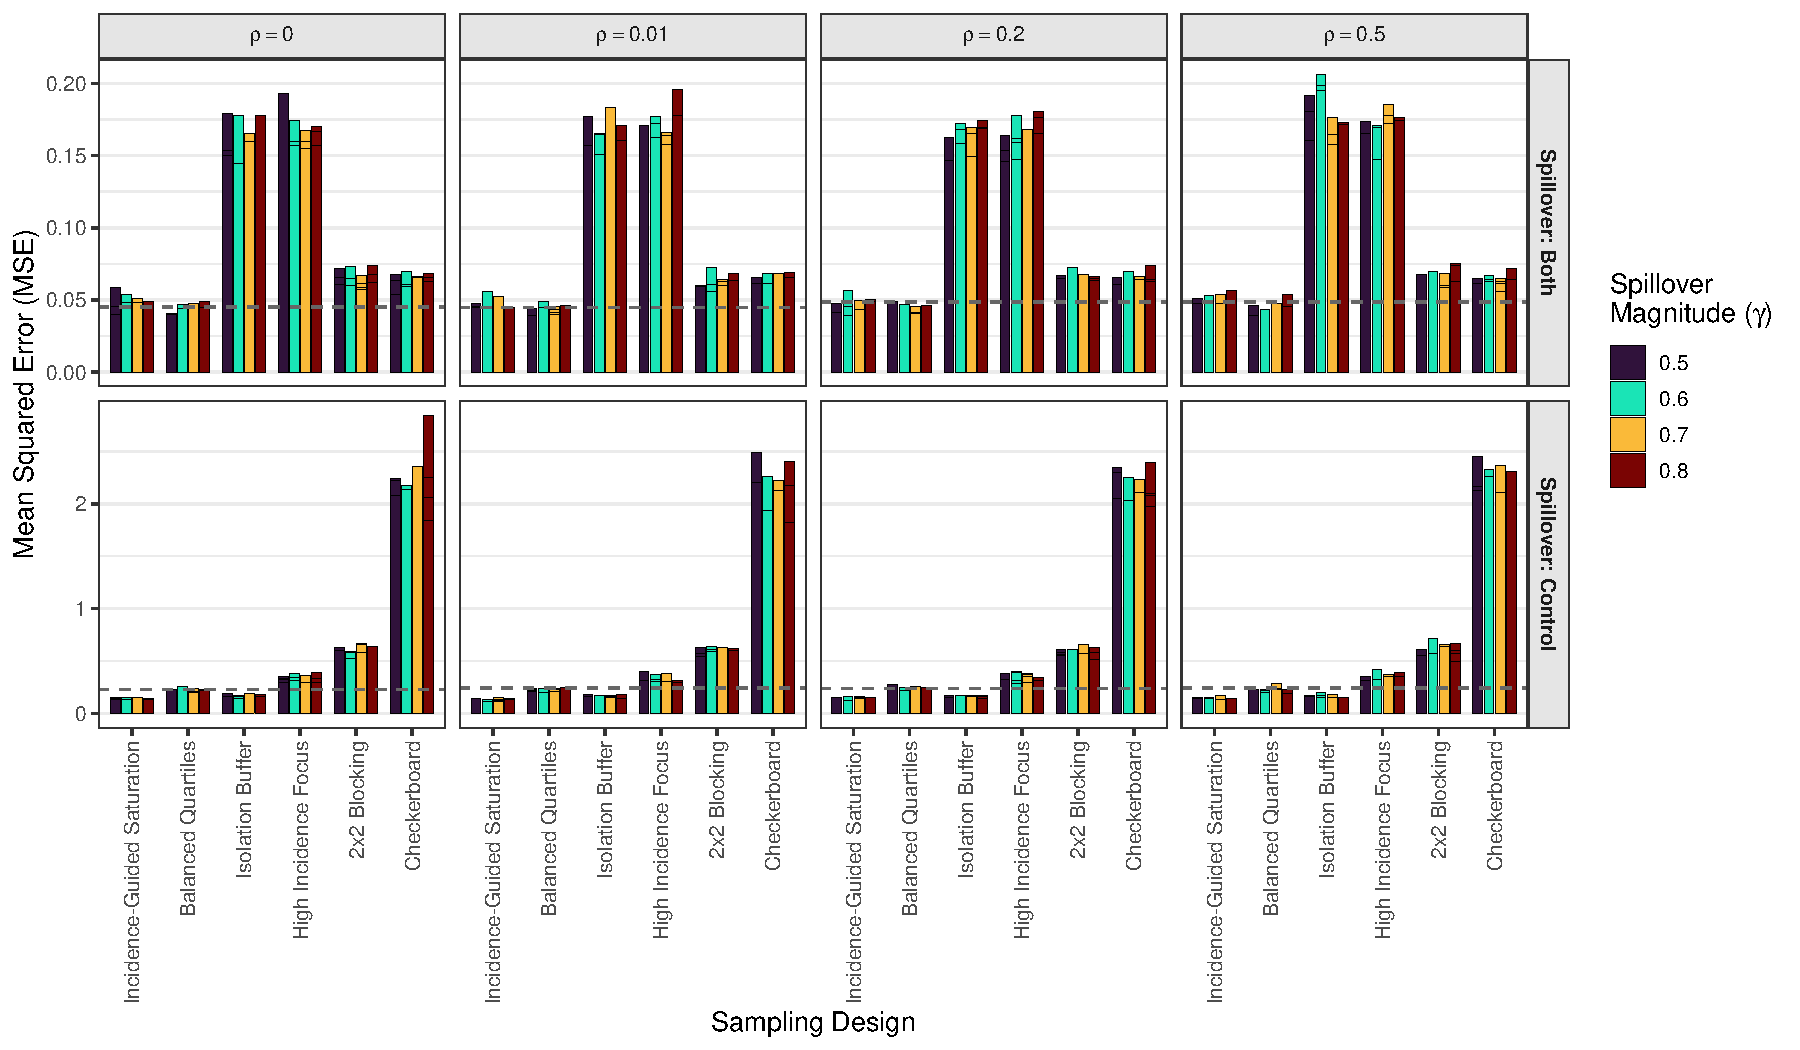
\includegraphics[width=0.79\linewidth]{../figures/fig_mse_by_design_ranked_6design_queen.pdf}

\caption{Mean squared error (MSE) of the oracle estimate of $\tau$ by design at $\tau = 1$, under queen contiguity. Columns of panels correspond to the four levels of outcome spatial dependence $\rho$, rows to the both-arms (top) and control-only (bottom) spillover regimes, and bar colors to the spillover magnitude $\gamma$. Each bar overlays the MSEs of the five incidence configurations for one combination of design, $\rho$, $\gamma$, and regime: the bar's height is the largest of the five, and the horizontal lines within it mark the other four. Designs are ordered by pooled mean MSE (Table \ref{tab:performance}). The gray dashed line in each panel marks simple random sampling (SRS), the largest of its five configuration MSEs averaged over the four values of $\gamma$. The vertical scale is set separately for each row. Figure \ref{fig:mse-rook} in Section \ref{app:rook-figures} shows rook contiguity.}
\label{fig:mse}

\end{figure}

\subsection{Formal statistical
comparison}\label{formal-statistical-comparison}

The Friedman test rejected equal MSE ranks across the six designs and SRS under
queen contiguity at \(\tau = 1\) (\(\chi^2 = 560.33\),
\(\text{df} = 6\), 160 blocks, \(p < 2.2\times10^{-16}\)). The average
within-block ranks were 1.78 for Incidence-Guided Saturation, 2.60 for SRS,
2.69 for Balanced Quartiles, 4.19 for Isolation Buffer, 5.24 for
\(2\times2\) Blocking, 5.74 for Checkerboard, and 5.76 for High
Incidence Focus. Nemenyi comparisons (critical difference 0.712)
separated 17 of the 21 pairs (Section \ref{app:supp-comparisons} shows
the critical-difference diagrams). Incidence-Guided Saturation
ranked significantly better than every other design and than SRS (\(p = 0.011\)). SRS and Balanced
Quartiles could not be distinguished from each other (\(p = 1.00\)), and both ranked significantly
better than the remaining four designs. The other three pairs that Nemenyi comparisons
did not separate all lay among the bottom three designs: \(2\times2\)
Blocking against High Incidence Focus (\(p = 0.32\)) and Checkerboard (\(p = 0.39\)), and Checkerboard
against High Incidence Focus (\(p = 1.00\)). Holm-adjusted Wilcoxon
signed-rank tests separated 20 of the 21 pairs, all except Balanced Quartiles against SRS (\(p = 0.15\)).

\begin{figure}[!htb]

\centering
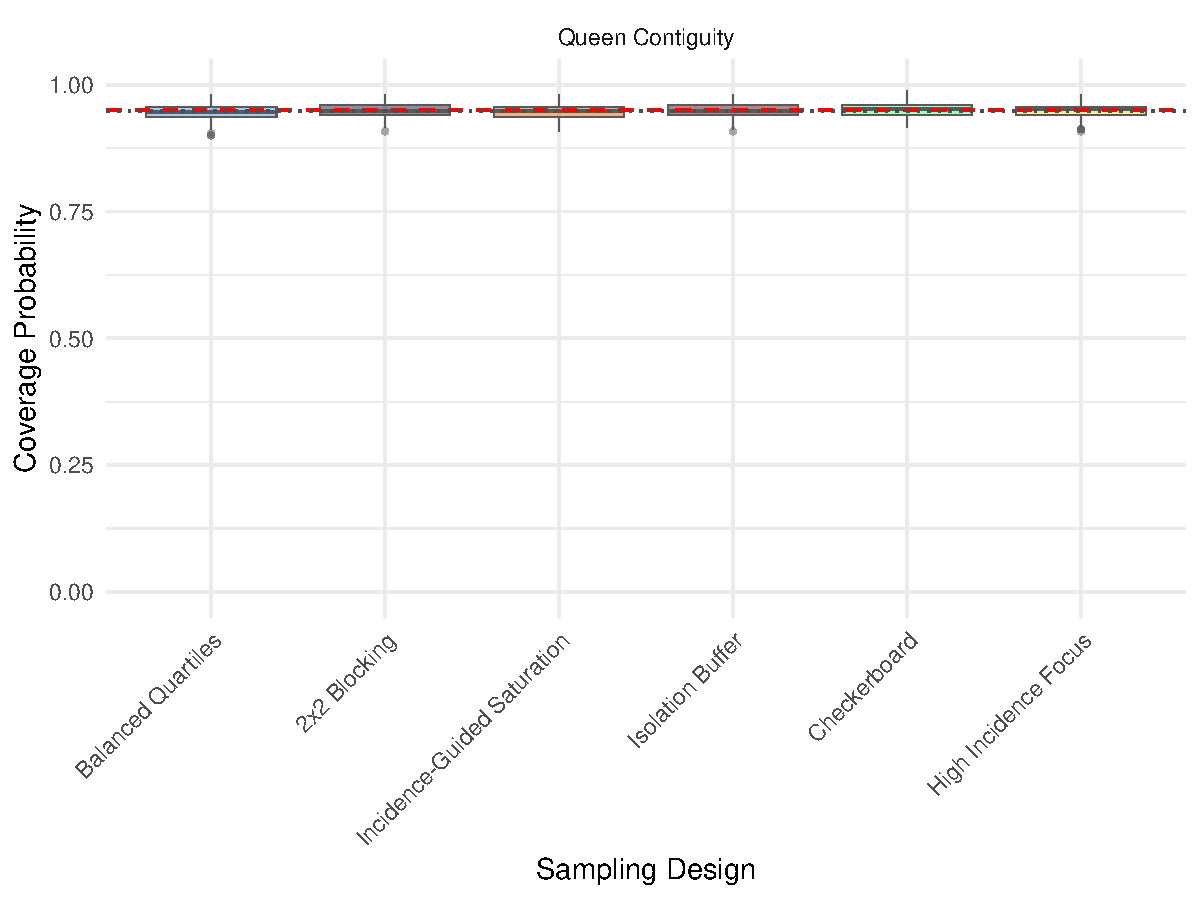
\includegraphics[width=0.6\linewidth]{../figures/fig_coverage_by_design_6design_queen.pdf}

\caption{Coverage of the 95\% confidence intervals by design at $\tau = 1$, under queen contiguity. Each box summarizes the coverage of the 160 scenarios of one design (5 incidence configurations $\times$ 4 values of $\rho$ $\times$ 4 values of $\gamma$ $\times$ 2 spillover regimes), each estimated from 250 fits. Designs are ordered by median coverage, so the order differs from the MSE order used elsewhere. The dashed red line marks the nominal 0.95 level, and the gray dotted line the median coverage of simple random sampling. Figure \ref{fig:coverage-rook} in Section \ref{app:rook-figures} shows rook contiguity.}
\label{fig:coverage}

\end{figure}

The bottom three designs were ordered differently by average rank and by
mean MSE. By mean MSE the order was High Incidence Focus (0.245),
\(2\times2\) Blocking (0.319), and Checkerboard (1.087); by average rank
it was \(2\times2\) Blocking (5.24), Checkerboard (5.74), and High
Incidence Focus (5.76). Both reversals have the same source: the MSEs of
\(2\times2\) Blocking and Checkerboard depended strongly on the
spillover regime. Each had a lower MSE than High Incidence Focus in all
80 both-arms blocks (mean MSE 0.062 for each, against 0.162) and a
higher MSE in all 80 control-only blocks (0.576 and 2.111, against
0.329; see the spillover-regime results below). Average rank counts each
block once, so their wins under the both-arms regime offset their losses
under the control-only regime; mean MSE weights those losses by their
size.

Because blocks within an incidence configuration share their ten
surfaces, we also compared each pair of designs adjacent in the mean-MSE
order over the 50 independent configuration-by-surface units. Every
adjacent pair differed significantly. The mean paired differences in
MSE, with \(t_{49}\) 95\% intervals, were \(-0.0401\) (\(-0.0431\),
\(-0.0372\)) for Incidence-Guided Saturation against Balanced
Quartiles, \(-0.0293\) (\(-0.0332\), \(-0.0255\)) for Balanced Quartiles
against Isolation Buffer, \(-0.0853\) (\(-0.0954\), \(-0.0752\)) for
Isolation Buffer against High Incidence Focus, \(-0.0738\) (\(-0.0858\),
\(-0.0617\)) for High Incidence Focus against \(2\times2\) Blocking, and
\(-0.7677\) (\(-0.7893\), \(-0.7460\)) for \(2\times2\) Blocking against
Checkerboard, with Wilcoxon \(p \le 4.9\times10^{-9}\) in every case.
The better design of each pair had the lower MSE in all 50 units, except
High Incidence Focus against \(2\times2\) Blocking, where it did so in
48 (96\%). This test follows the mean-MSE order. It separated High
Incidence Focus from \(2\times2\) Blocking, which the Nemenyi comparison
of within-block ranks did not, because each unit's MSE averages over
both spillover regimes, and there the control-only losses of
\(2\times2\) Blocking outweigh its both-arms wins.

\subsection{Design rankings by incidence
configuration}\label{design-rankings-by-incidence-configuration}

Table \ref{tab:by-config} gives each design's MSE within each of the
five incidence configurations. Under queen contiguity, the mean-MSE
order within every configuration was the same as the pooled order:
Incidence-Guided Saturation, Balanced Quartiles, Isolation
Buffer, High Incidence Focus, \(2\times2\) Blocking, and Checkerboard.
The configuration changed each design's MSE only slightly: in this
order, each design's highest MSE across the five configurations was
lower than the next design's lowest. Incidence-Guided Saturation had the lowest MSE in 18 to 21 of the 32 blocks in each
configuration. Coverage did not depend on the configuration either:
within each configuration, every design's coverage, averaged over its 32
scenarios, was between 0.941 and 0.952. The mechanism that generated the
incidence surface therefore did not change the ranking. This includes
High Incidence Focus, the design that uses the incidence ranks most
directly: its MSE was no higher under the two Poisson configurations
than under the iid and spatial configurations.

\begin{table}[!htb]

\small
\centering
\setlength{\tabcolsep}{4pt}

\caption{Mean squared error by design within each of the five incidence configurations at $\tau = 1$, under queen contiguity (primary) and rook contiguity (sensitivity). Each entry averages the 32 scenarios of one design, neighbor type, and configuration (4 values of $\rho$ $\times$ 4 values of $\gamma$ $\times$ 2 spillover regimes), each summarizing 250 fits of the oracle model. The spatially autocorrelated and Poisson configurations are labeled by the strength of dependence in the incidence surface, $\rho_X$. Rows in both panels are ordered by pooled mean MSE under queen contiguity (Table \ref{tab:performance}). Under rook contiguity, $\tau$ is not identified for Checkerboard; its estimates are kept and flagged.}
\label{tab:by-config}

\begin{tabular}{lccccc}

\toprule
& & \multicolumn{2}{c}{Spatial} & \multicolumn{2}{c}{Poisson} \\
\cmidrule(lr){3-4}\cmidrule(lr){5-6}
Design & iid & $\rho_X=0.20$ & $\rho_X=0.50$ & $\rho_X=0.20$ & $\rho_X=0.50$ \\

\midrule
\multicolumn{6}{l}{\textit{Queen contiguity}} \\
Incidence-Guided Saturation & 0.093 & 0.087 & 0.092 & 0.090 & 0.092 \\
Balanced Quartiles & 0.130 & 0.130 & 0.131 & 0.128 & 0.135 \\
Isolation Buffer & 0.160 & 0.159 & 0.159 & 0.162 & 0.161 \\
High Incidence Focus & 0.245 & 0.267 & 0.245 & 0.232 & 0.238 \\
2$\times$2 Blocking & 0.311 & 0.315 & 0.323 & 0.326 & 0.320 \\
Checkerboard & 1.091 & 1.068 & 1.086 & 1.112 & 1.077 \\

\midrule
\multicolumn{6}{l}{\textit{Rook contiguity}} \\
Incidence-Guided Saturation & 0.072 & 0.072 & 0.073 & 0.073 & 0.069 \\
Balanced Quartiles & 0.081 & 0.084 & 0.084 & 0.084 & 0.085 \\
Isolation Buffer & 0.131 & 0.131 & 0.132 & 0.136 & 0.134 \\
High Incidence Focus & 0.205 & 0.213 & 0.200 & 0.202 & 0.211 \\
2$\times$2 Blocking & 0.129 & 0.125 & 0.129 & 0.130 & 0.129 \\
Checkerboard (flagged) & 0.480 & 0.482 & 0.474 & 0.481 & 0.482 \\

\bottomrule

\end{tabular}

\end{table}

\subsection{Spatial dependence, spillover magnitude and regime}\label{sensitivity-to-spatial-dependence-spillover-magnitude-and-spillover-regime}

Under queen contiguity, neither the strength of spatial dependence in
the outcome nor the spillover magnitude changed the ranking. Across
\(\rho \in \{0, 0.01, 0.20, 0.50\}\), no design's MSE changed by more
than 0.02 (Table \ref{tab:rho}). Across
\(\gamma \in \{0.5, 0.6, 0.7, 0.8\}\), the MSE of every design except
Checkerboard also varied by less than 0.02, and Checkerboard's varied
between 1.052 and 1.108 with no trend in \(\gamma\) (Table
\ref{tab:gamma}). Under rook contiguity, \(\gamma\) mattered for
Checkerboard alone, for the reason given in the rook results below.

\begin{table}[!htb]

\small
\centering

\caption{Mean squared error by design across the four levels of outcome spatial dependence $\rho$, under queen contiguity at $\tau = 1$, pooled over the five incidence configurations. Each entry averages 40 scenarios (5 incidence configurations $\times$ 4 values of $\gamma$ $\times$ 2 spillover regimes). Rows are ordered by pooled mean MSE under queen contiguity (Table \ref{tab:performance}).}
\label{tab:rho}

\begin{tabular}{lcccc}

\toprule
Design & $\rho=0$ & $\rho=0.01$ & $\rho=0.20$ & $\rho=0.50$ \\

\midrule
Incidence-Guided Saturation & 0.090 & 0.087 & 0.093 & 0.093 \\
Balanced Quartiles & 0.129 & 0.129 & 0.132 & 0.133 \\
Isolation Buffer & 0.161 & 0.157 & 0.158 & 0.165 \\
High Incidence Focus & 0.243 & 0.242 & 0.249 & 0.248 \\
2$\times$2 Blocking & 0.318 & 0.320 & 0.314 & 0.324 \\
Checkerboard & 1.095 & 1.077 & 1.084 & 1.092 \\

\bottomrule

\end{tabular}

\end{table}

\begin{table}[!htb]

\small
\centering

\caption{Mean squared error by design across the four levels of spillover magnitude $\gamma$ at $\tau = 1$, under queen contiguity (primary) and rook contiguity (sensitivity), pooled over the five incidence configurations. Each entry averages 40 scenarios (5 incidence configurations $\times$ 4 values of $\rho$ $\times$ 2 spillover regimes). Rows in both panels are ordered by pooled mean MSE under queen contiguity (Table \ref{tab:performance}). Under rook contiguity, $\tau$ is not identified for Checkerboard; its estimates are kept and flagged.}
\label{tab:gamma}

\begin{tabular}{lcccc}

\toprule
Design & $\gamma=0.5$ & $\gamma=0.6$ & $\gamma=0.7$ & $\gamma=0.8$ \\

\midrule
\multicolumn{5}{l}{\textit{Queen contiguity}} \\
Incidence-Guided Saturation & 0.092 & 0.089 & 0.092 & 0.089 \\
Balanced Quartiles & 0.132 & 0.128 & 0.132 & 0.131 \\
Isolation Buffer & 0.159 & 0.163 & 0.160 & 0.159 \\
High Incidence Focus & 0.244 & 0.249 & 0.248 & 0.241 \\
2$\times$2 Blocking & 0.312 & 0.314 & 0.328 & 0.323 \\
Checkerboard & 1.108 & 1.052 & 1.086 & 1.101 \\

\midrule
\multicolumn{5}{l}{\textit{Rook contiguity}} \\
Incidence-Guided Saturation & 0.069 & 0.072 & 0.075 & 0.072 \\
Balanced Quartiles & 0.083 & 0.085 & 0.083 & 0.083 \\
Isolation Buffer & 0.131 & 0.133 & 0.134 & 0.133 \\
High Incidence Focus & 0.207 & 0.209 & 0.205 & 0.203 \\
2$\times$2 Blocking & 0.129 & 0.129 & 0.127 & 0.128 \\
Checkerboard (flagged) & 0.295 & 0.403 & 0.538 & 0.684 \\

\bottomrule

\end{tabular}

\end{table}

The spillover regime was the one factor that changed the queen ranking
(Table \ref{tab:regime}, Figure \ref{fig:mse}). Under the both-arms
regime, Balanced Quartiles had the lowest MSE (0.042), followed by
Incidence-Guided Saturation (0.046), \(2\times2\) Blocking
(0.062), Checkerboard (0.062), Isolation Buffer (0.161), and High
Incidence Focus (0.162). Under the control-only regime, the order was
Incidence-Guided Saturation (0.135), Isolation Buffer (0.159),
Balanced Quartiles (0.219), High Incidence Focus (0.329), \(2\times2\)
Blocking (0.576), and Checkerboard (2.111); at larger values of
\(\tau\), Isolation Buffer matched or passed Incidence-Guided Saturation under this regime (see Stability across treatment effect
sizes). For Isolation Buffer, no treated cluster has a treated neighbor,
so \(WZ = 0\) at every treated cluster and \(WZ \circ (1 - Z) = WZ\).
The two regimes in Equation \ref{eq:spillover} therefore define the same
outcome model, and so the same expected MSE; the observed values, 0.161
and 0.159, differ only by Monte Carlo error, because the two regimes use
separate draws. Every other design had a higher MSE under the
control-only regime, and the increase was largest for Checkerboard and
\(2\times2\) Blocking, which went from close to the best designs under
the both-arms regime to the two worst under the control-only regime.
Among the six detailed designs, Incidence-Guided Saturation was first or second under both regimes, at this and every other value of $\tau$. In the full benchmark that includes SRS (Table \ref{tab:grid-srs}), its both-arms MSE was 8\% above that of SRS, a small but statistically detectable difference (Figure \ref{fig:vs-srs}). This matters because a trial team may not know in advance which regime applies.

\begin{table}[!htb]

\small
\centering
\setlength{\tabcolsep}{4pt}

\caption{Mean squared error by design under each spillover regime at $\tau = 1$, under queen contiguity (primary) and rook contiguity (sensitivity), pooled over the five incidence configurations. Each entry averages 80 scenarios (5 incidence configurations $\times$ 4 values of $\rho$ $\times$ 4 values of $\gamma$). Rows are ordered by pooled mean MSE under queen contiguity (Table \ref{tab:performance}). Under rook contiguity, $\tau$ is not identified for Checkerboard; its estimates are kept and flagged.}
\label{tab:regime}

\begin{tabular}{lcccc}

\toprule
& \multicolumn{2}{c}{Queen} & \multicolumn{2}{c}{Rook} \\
Design & Both arms & Control only & Both arms & Control only \\

\midrule
Incidence-Guided Saturation & 0.046 & 0.135 & 0.045 & 0.098 \\
Balanced Quartiles & 0.042 & 0.219 & 0.042 & 0.125 \\
Isolation Buffer & 0.161 & 0.159 & 0.131 & 0.134 \\
High Incidence Focus & 0.162 & 0.329 & 0.164 & 0.249 \\
2$\times$2 Blocking & 0.062 & 0.576 & 0.051 & 0.206 \\
Checkerboard (flagged under rook) & 0.062 & 2.111 & 0.477 & 0.483 \\

\bottomrule

\end{tabular}

\end{table}

The increase under the control-only regime was variance, not bias. The
oracle model includes the true regime-specific spillover covariate, so
it has no omitted-variable bias. At \(\tau = 1\), in every combination
of design and regime under queen contiguity, the absolute bias was at
most 0.048 and squared bias, averaged over scenarios, was at most 2.2\%
of MSE. Checkerboard showed the mechanism most clearly: under the
control-only regime its spillover covariate is a linear combination of
the intercept and \(Z\) at every interior cluster, so only the boundary
clusters separate the spillover effect from the treatment effect
(Methods). Checkerboard's MSE rose from 0.062 under the both-arms regime
to 2.111 under the control-only regime, while its bias stayed near zero
(0.004) and its coverage stayed at 0.951: its intervals widened with its
variance. Its pooled MSE of 1.087 was almost entirely variance: squared
bias, averaged over scenarios, was 0.0045, less than 0.5\% of MSE
(Figure \ref{fig:biasvar} shows the decomposition for the Poisson
configuration with \(\rho_X = 0.20\)). \(2\times2\) Blocking showed the
same pattern on a smaller scale, with MSE rising from 0.062 to 0.576 and
a bias of 0.016 under the control-only regime.

\begin{figure}[!htb]

\centering
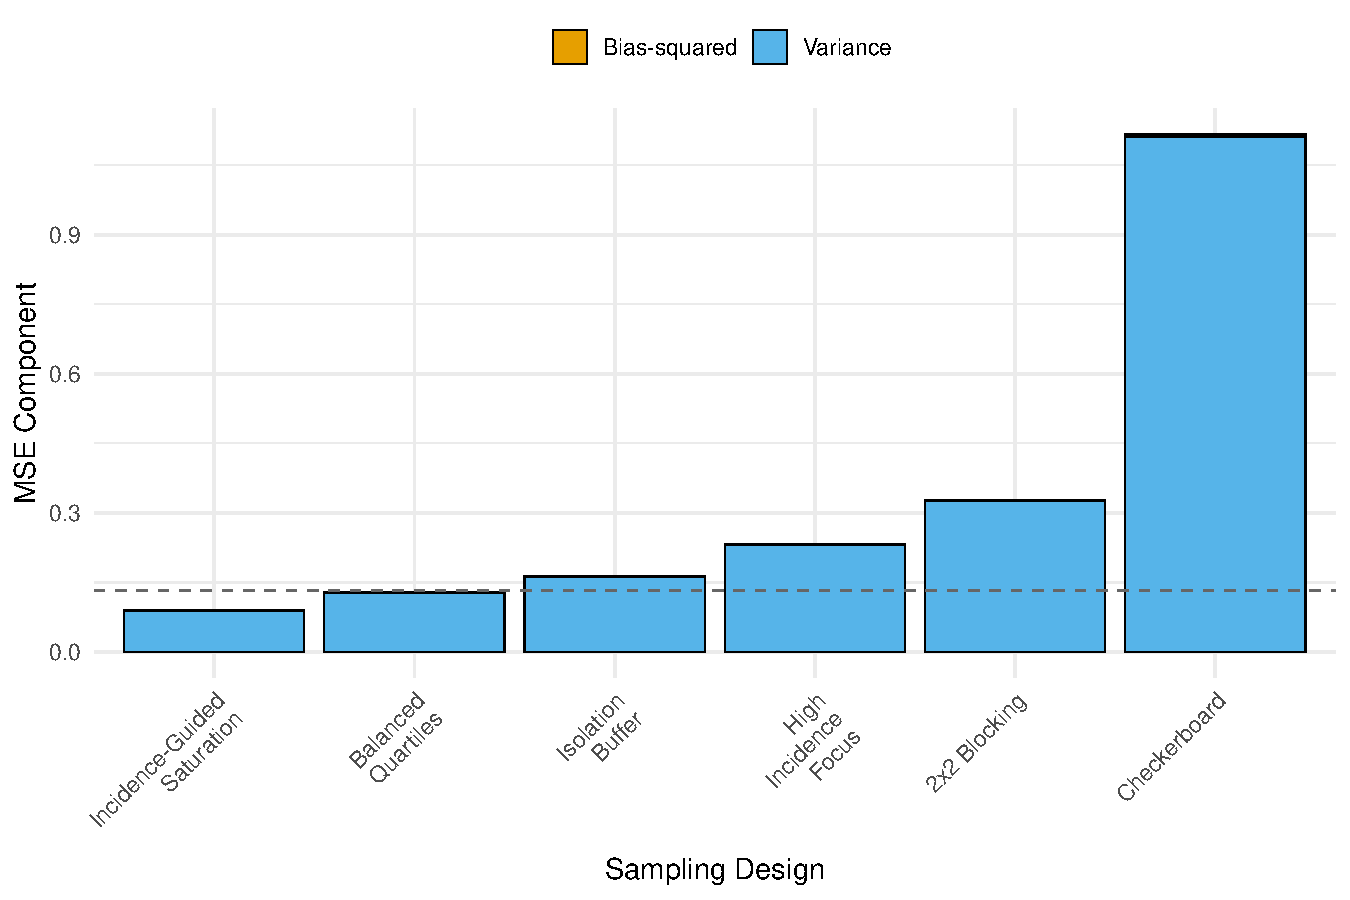
\includegraphics[width=0.62\linewidth]{../figures/fig_biasvar_6design_queen.pdf}

\caption{Decomposition of mean squared error into squared bias and variance by design at $\tau = 1$ for one incidence configuration, Poisson with $\rho_X = 0.20$, under queen contiguity. For each design, the two stacked components are the squared bias and the variance ($\text{SD}^2$) of $\hat\tau$, each averaged over the 32 scenarios of that configuration (4 values of $\rho$ $\times$ 4 values of $\gamma$ $\times$ 2 spillover regimes). Designs are ordered by pooled mean MSE (Table \ref{tab:performance}). The gray dashed line marks the MSE of simple random sampling (SRS) in the same configuration. Figure \ref{fig:biasvar-rook} in Section \ref{app:rook-figures} shows rook contiguity.}
\label{fig:biasvar}

\end{figure}

\subsection{Rook contiguity}\label{rook-contiguity}

Under rook contiguity at \(\tau = 1\), pooled over the five incidence
configurations, the mean-MSE order was Incidence-Guided Saturation (0.072), Balanced Quartiles (0.084), \(2\times2\) Blocking
(0.128), Isolation Buffer (0.133), High Incidence Focus (0.206), and
Checkerboard (0.480) (Table \ref{tab:performance}; Figure
\ref{fig:mse-rook} in Section \ref{app:rook-figures}), and the same
order held within each of the five incidence configurations (Table
\ref{tab:by-config}). Incidence-Guided Saturation had the
lowest MSE in 97 of the 160 rook blocks (61\%) and Balanced Quartiles in
60 (38\%). Coverage was between 0.948 and 0.952 for every design except Checkerboard, whose coverage was 0.162 (Figure \ref{fig:coverage-rook}
in Section \ref{app:rook-figures}); within single incidence
configurations, the corresponding ranges were 0.944 to 0.954, and 0.15 to 0.16 for Checkerboard. With SRS as a seventh member, the Friedman test rejected equal ranks
(\(\chi^2 = 795.77\), \(\text{df} = 6\), 160 blocks,
\(p < 2.2\times10^{-16}\)). Nemenyi comparisons separated 17 of 21
pairs; the four they did not separate were Incidence-Guided Saturation against Balanced Quartiles (\(p = 0.66\)) and SRS (\(p = 0.14\)), Balanced Quartiles against SRS (\(p = 0.97\)), and \(2\times2\)
Blocking against Isolation Buffer (\(p = 1.00\)). Holm-adjusted Wilcoxon
tests separated every pair except \(2\times2\) Blocking against
Isolation Buffer and Balanced Quartiles against SRS (both \(p = 0.21\)). In the surface-level comparison, Incidence-Guided
Saturation had a lower MSE than Balanced Quartiles in 48 of
the 50 units (mean difference \(-0.0121\); \(-0.0139\), \(-0.0102\);
Wilcoxon \(p = 9.9\times10^{-10}\)). \(2\times2\) Blocking and Isolation
Buffer were close: \(2\times2\) Blocking had the lower MSE in 36 of the
50 units (72\%; mean difference \(-0.0048\); \(-0.0078\), \(-0.0017\);
Wilcoxon \(p = 0.0027\)), but Isolation Buffer had the slightly better
average rank (4.21 against 4.33), and the two designs traded places in mean MSE at
\(\tau = 3\) (see the results for \(\tau\) below). Every
other adjacent pair differed in all 50 units.

Checkerboard under rook contiguity is a different case: \(\tau\) is not
identified, and the coefficient on \(Z\) estimates \(\tau - \gamma\)
(Methods). The estimates behaved accordingly. At \(\tau = 1\),
Checkerboard's mean bias was \(-0.502\), \(-0.600\), \(-0.704\), and
\(-0.802\) at \(\gamma = 0.5\), 0.6, 0.7, and 0.8, while its mean
standard deviation stayed between 0.20 and 0.21; squared bias, averaged
over scenarios, accounted for 0.438 of its MSE of 0.480 (Figure
\ref{fig:biasvar-rook} in Section \ref{app:rook-figures} shows the
decomposition for the Poisson configuration with \(\rho_X = 0.20\)). Its
coverage fell from 0.337 at \(\gamma = 0.5\) to 0.031 at
\(\gamma = 0.8\). Because \(WZ = 1 - Z\), the two spillover covariates
in Equation \ref{eq:spillover} coincide,
\(\gamma\, WZ \circ (1 - Z) = \gamma(1 - Z) = \gamma\, WZ\), so the two
regimes define the same outcome model and the same expected MSE; the
observed values, 0.477 under the both-arms regime and 0.483 under the
control-only regime, differ only by Monte Carlo error, because the two
regimes use separate noise draws. Under queen contiguity, by contrast,
Checkerboard's coverage stayed between 0.949 and 0.952 at every level of \(\rho\); under rook contiguity it was between 0.146 and 0.171 (Table
\ref{tab:checkerboard-coverage}). Rook Checkerboard estimates were
precise but centered on the wrong quantity, the opposite of its
imprecise but valid queen estimates. We keep these estimates in every
ranking and flag them.

\begin{table}[!htb]

\small
\centering

\caption{Checkerboard's 95\% confidence interval coverage across the four levels of outcome spatial dependence $\rho$ at $\tau = 1$, under queen contiguity (primary) and rook contiguity (sensitivity), pooled over the five incidence configurations. Each entry averages 40 scenarios (5 incidence configurations $\times$ 4 values of $\gamma$ $\times$ 2 spillover regimes). Under rook contiguity, $\tau$ is not identified for Checkerboard; its estimates are kept and flagged. The nominal level is 0.95.}
\label{tab:checkerboard-coverage}

\begin{tabular}{lcccc}

\toprule
Neighbor type & $\rho=0$ & $\rho=0.01$ & $\rho=0.20$ & $\rho=0.50$ \\

\midrule
Queen & 0.950 & 0.952 & 0.949 & 0.949 \\
Rook & 0.171 & 0.168 & 0.161 & 0.146 \\

\bottomrule

\end{tabular}

\end{table}

\subsection{Non-oracle sensitivity
analysis}\label{non-oracle-sensitivity-analysis}

The non-oracle model, which omits the spillover term, was biased for
every design (Table \ref{tab:oracle-nonoracle} in Section
\ref{app:oracle-nonoracle} gives both models' MSE, bias, and coverage
for each design). At \(\tau = 1\), and setting aside Checkerboard under
rook contiguity, its bias ranged from \(-0.12\) to \(-0.40\) and its
coverage from 0.54 to 0.91 across designs and neighbor types. Under
queen contiguity its bias ranged from \(-0.123\) (Incidence-Guided
Saturation) to \(-0.244\) (\(2\times2\) Blocking) and its
coverage from 0.727 (\(2\times2\) Blocking) to 0.907 (High Incidence Focus); under rook contiguity the most biased design other than
Checkerboard was Isolation Buffer (bias \(-0.400\), coverage 0.536). For
Checkerboard under rook contiguity, the non-oracle estimates were
identical to the oracle estimates (MSE 0.480, bias \(-0.652\), coverage 0.162), because once the aliased spillover column is dropped the two
models are the same.

Omitting the spillover term also removes a column that can be nearly
collinear with \(Z\), and the non-oracle estimates were accordingly less
variable for some designs. Under queen contiguity, the non-oracle MSE
was lower than the oracle MSE for every design, most of all for
Checkerboard (oracle 1.087, non-oracle 0.108) and \(2\times2\) Blocking
(oracle 0.319, non-oracle 0.121). Under rook contiguity it was higher
for every design except \(2\times2\) Blocking (0.128 under both models)
and Checkerboard (identical). These results do not change the
recommendation. Incidence-Guided Saturation also had the
lowest non-oracle MSE under both neighbor types (0.087 under queen
contiguity and 0.086 under rook contiguity), and where a design's
non-oracle MSE was lower, the estimate was biased and its intervals
under-covered, so the lower MSE does not support valid inference.

\subsection{Stability across treatment effect
sizes}\label{stability-across-treatment-effect-sizes}

Under queen contiguity, each of the two design orders was the same at
every tested value of \(\tau\) (0.8, 1.0, 1.5, 2.0 and 3.0): the order by average
within-block rank did not change across these values, and neither did
the order by mean MSE, although the two orders differ from each other in
the bottom three designs (see Formal statistical comparison; Figure
\ref{fig:tau-mse}a shows mean MSE). With SRS included, the order by average rank placed SRS second at every value of \(\tau\), and the Friedman statistic was 564.09,
560.33, 540.92, 526.55, and 497.55 at these five values
(\(p < 2.2\times10^{-16}\) at each). Under rook contiguity the order was
also stable (Figure \ref{fig:tau-mse}b). By average rank among the six designs and SRS, it was the same at every value of \(\tau\), with SRS third behind Incidence-Guided Saturation and Balanced Quartiles. By mean MSE, the close pair of
\(2\times2\) Blocking and Isolation Buffer traded places, with
Isolation Buffer ahead only at \(\tau = 3\). The five values of
\(\tau\) share their assignments and noise, so these five comparisons
are not independent confirmations of one another; they show that, under
queen contiguity, the order did not change across the five values of
\(\tau\) we tested, given the same draws.

\begin{figure}[!htb]

\centering
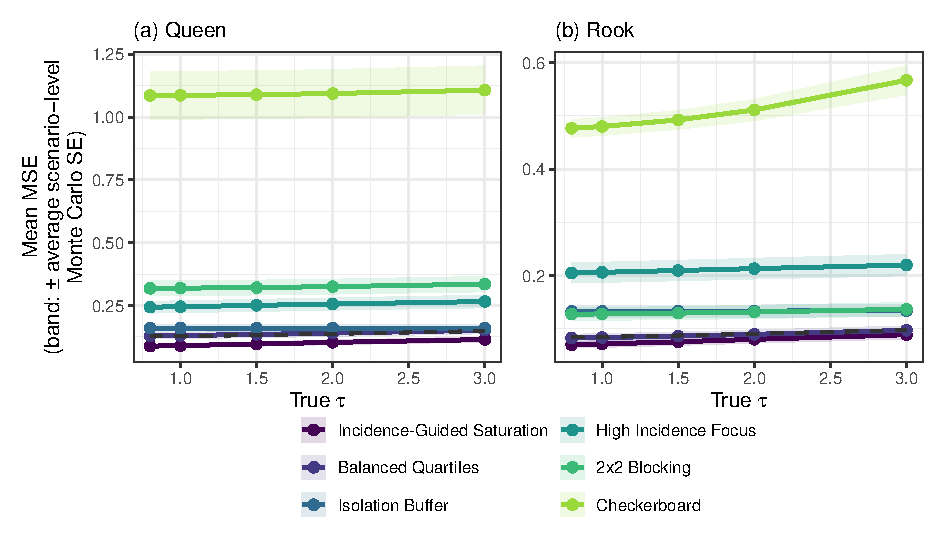
\includegraphics[width=0.9\linewidth]{../figures/fig_tau_sensitivity_6design_combined.pdf}

\caption{Mean squared error by design across the five values of the treatment effect, $\tau \in \{0.8, 1.0, 1.5, 2.0, 3.0\}$, under (a) queen contiguity (primary) and (b) rook contiguity (sensitivity). Each point averages the 160 scenarios of one design at one value of $\tau$, pooled over the five incidence configurations. Shaded bands show $\pm 1$ times the average of the scenario-level Monte Carlo standard errors of MSE; they describe the precision of a single scenario's MSE, not of the plotted average, whose standard error is smaller (Table \ref{tab:performance}). The shared legend lists the designs in order of pooled mean MSE under queen contiguity at $\tau = 1$. The vertical scales of the two panels differ. The gray dashed line marks simple random sampling (SRS). Under rook contiguity, $\tau$ is not identified for Checkerboard; its estimates are kept and flagged. The five values of $\tau$ share their assignments and noise.}
\label{fig:tau-mse}

\end{figure}

Within that stable order, the margins moved. Under queen contiguity, the
average rank of Incidence-Guided Saturation rose from 1.41 at
\(\tau = 0.8\) to 1.85 at \(\tau = 3\), but Balanced Quartiles did not
gain on it: Incidence-Guided Saturation had the lower MSE of
the two in 103, 102, 102, 102, and 101 of the 160 blocks at
\(\tau = 0.8\), 1, 1.5, 2, and 3, and the average rank of Balanced
Quartiles stayed between 2.13 and 2.14. Isolation Buffer gained instead,
and its average rank fell from 3.71 to 3.31. The MSE of Isolation Buffer
stayed at 0.160 at every value of \(\tau\), while that of
Incidence-Guided Saturation rose from 0.088 to 0.115 and that
of Balanced Quartiles from 0.130 to 0.152, so the gap between
Incidence-Guided Saturation and Balanced Quartiles stayed
between 0.037 and 0.041. Isolation Buffer's gain came under the
control-only regime, where Incidence-Guided Saturation had a
lower MSE than Isolation Buffer in 75, 73, 56, 40, and 12 of the 80
blocks at the five values of \(\tau\). The mean control-only MSE of
Incidence-Guided Saturation rose from 0.131 at \(\tau = 0.8\)
to 0.182 at \(\tau = 3\), while that of Isolation Buffer stayed between
0.159 and 0.160 (Section \ref{app:technical-notes}). At \(\tau = 2\) the
two were level (0.1596 for Isolation Buffer against 0.1604), and at
\(\tau = 3\) Isolation Buffer had the lower control-only MSE (0.160
against 0.182). Incidence-Guided Saturation remained second
under the control-only regime at those two values, second to Balanced
Quartiles under the both-arms regime at every value of \(\tau\), and
lowest in pooled MSE at every value of \(\tau\). Its worst case across
blocks was the lowest of the six designs at \(\tau \le 1.5\), but at
\(\tau = 2\) and \(\tau = 3\) that of Isolation Buffer was lower (0.207
against 0.210, and 0.208 against 0.238). The mean bias of
Incidence-Guided Saturation also grew with \(\tau\), from
0.029 at \(\tau = 0.8\) to 0.047 at \(\tau = 3\), but squared bias,
averaged over scenarios, stayed at or below 3.0\% of its MSE, so the
rise in its MSE was mostly variance.

Under rook contiguity, Incidence-Guided Saturation kept the
lowest control-only MSE at every value of \(\tau\), although its margin
over Isolation Buffer narrowed, from 0.095 against 0.134 at
\(\tau = 0.8\) to 0.131 against 0.136 at \(\tau = 3\), where it had the
lower MSE in 47 of the 80 control-only blocks. Its worst case across
rook blocks was the lowest of the six designs at every value of \(\tau\)
except \(\tau = 3\), where that of Isolation Buffer was lower (0.173
against 0.174).

Except for Checkerboard under rook contiguity, coverage stayed close to 0.95 at every value of \(\tau\). Pooled over the five incidence
configurations, every design's coverage was between 0.946 and 0.950 at every value of \(\tau\) under queen contiguity, and every design except Checkerboard was between 0.947 and 0.952 at every value of \(\tau\)
under rook contiguity. The coverage of rook Checkerboard, for which
\(\tau\) is not identified, rose from 0.150 at \(\tau = 0.8\) to 0.162, 0.212, 0.286, and 0.464 at \(\tau = 1\), 1.5, 2, and 3 (Section
\ref{app:technical-notes}). Section \ref{app:supp-comparisons} shows
coverage across \(\tau\) for each design.

\subsection{Robustness across blocks and the recommended
design}\label{robustness-across-blocks-and-the-recommended-design}

Table \ref{tab:robustness} gives the distribution of MSE across the 160
queen blocks at \(\tau = 1\). Incidence-Guided Saturation had
the lowest median (0.080) and the lowest worst-case MSE of any design
(0.169). Isolation Buffer had the narrowest range (0.128 to 0.206),
because its MSE does not depend on the spillover regime, but at a higher
level. Balanced Quartiles had a low median (0.115) and a worst case of
0.290. The distributions of \(2\times2\) Blocking and Checkerboard
reflected their dependence on the spillover regime: both had low first
quartiles (0.062 and 0.063) and high upper quartiles (0.580 and 2.093).
Checkerboard had the highest MSE in all 80 control-only blocks; in the
80 both-arms blocks, the highest MSE belonged to High Incidence Focus in
42 and to Isolation Buffer in 38. Under rook contiguity,
Incidence-Guided Saturation also had the lowest worst-case MSE
(0.138).

\begin{table}[!htb]

\small
\centering

\caption{Distribution of block-level mean squared error by design across the 160 blocks under queen contiguity at $\tau = 1$, pooled over the five incidence configurations (32 blocks in each). At a fixed value of $\tau$, each block contributes one scenario per design. Rows are sorted by median, which here coincides with the order of pooled mean MSE under queen contiguity (Table \ref{tab:performance}).}
\label{tab:robustness}

\begin{tabular}{lccccc}

\toprule
Design & Best & Q25 & Median & Q75 & Worst \\

\midrule
Incidence-Guided Saturation & 0.037 & 0.045 & 0.080 & 0.135 & 0.169 \\
Balanced Quartiles & 0.034 & 0.042 & 0.115 & 0.221 & 0.290 \\
Isolation Buffer & 0.128 & 0.150 & 0.159 & 0.169 & 0.206 \\
High Incidence Focus & 0.139 & 0.160 & 0.234 & 0.322 & 0.424 \\
2$\times$2 Blocking & 0.048 & 0.062 & 0.271 & 0.580 & 0.719 \\
Checkerboard & 0.051 & 0.063 & 0.899 & 2.093 & 2.843 \\

\bottomrule

\end{tabular}

\end{table}

Among the six designs in the detailed comparison, Incidence-Guided
Saturation combines low pooled MSE with comparatively favorable
control-only performance. The SRS benchmark below changes the practical
interpretation: recommend the saturation approach when control-only
spillover is plausible, while retaining SRS as a competitive option
under both-arms spillover. Saturation Quadrants performed similarly, so incidence guidance lets a trial direct its highest treatment saturations to the highest-incidence regions with little or no loss of estimation accuracy. Scenario-level worst cases summarize variation across
parameter settings; they are distinct from conditional risk across
assignments within one setting.

\subsection{SRS benchmark and allocation-specific
risk}\label{srs-benchmark-and-allocation-specific-risk}

At \(\tau=1\) under queen contiguity, pooled over the five incidence
configurations and all spatial/spillover settings, Incidence-Guided Saturation has
mean MSE 0.0907 against SRS 0.1285; Saturation Quadrants has 0.0900. Table
\ref{tab:grid-srs} separates the regimes and includes all eight
strategies. Incidence-Guided Saturation's control-only ratio to SRS is 0.631,
whereas its both-arms ratio is 1.083. SRS, Balanced Quartiles and
Balanced Halves have similar both-arms accuracy. Small mean differences
should not be interpreted as equivalence, nor should pooling the regimes
obscure the difference in design guidance.

Figure \ref{fig:vs-srs} tests each design against SRS within each regime, over the 50 independent configuration-by-surface units. Under control-only spillover, Incidence-Guided Saturation had 36.9\% lower MSE than SRS (95\% interval 34.5\% to 39.2\% lower), Saturation Quadrants 36.7\% lower and Isolation Buffer 25.7\% lower, each in all 50 units (Holm-adjusted $p = 6.2\times10^{-9}$). Under both-arms spillover, Incidence-Guided Saturation had 8.3\% higher MSE than SRS (5.6\% to 11.0\% higher; $p = 6.1\times10^{-6}$) and Saturation Quadrants 4.3\% higher ($p = 0.017$). Balanced Quartiles and Balanced Halves did not differ significantly from SRS under either regime, and the remaining designs had significantly higher MSE than SRS under both-arms spillover, as did High Incidence Focus, $2\times2$ Blocking and Checkerboard under control-only spillover. The advantage of the saturation designs over SRS is therefore specific to control-only spillover, and under queen contiguity their small both-arms disadvantage is statistically detectable. Under rook contiguity the saturation designs had 23\% to 24\% lower control-only MSE than SRS and 3\% to 5\% higher both-arms MSE, significant for Incidence-Guided Saturation ($p = 0.0075$) but not for Saturation Quadrants ($p = 0.15$), and Isolation Buffer had 5.8\% higher control-only MSE than SRS. The mean is only part of the comparison, because a trial realizes a single allocation. Under control-only spillover, the worst 10\% of SRS allocations in the grid pilot had mean conditional MSE 60\% above that of the average SRS allocation (0.3486 against 0.2172), and the saturation designs' worst-decile MSE was 0.53 to 0.56 times SRS's in the grid pilot and 0.64 to 0.68 times in NC. Under both-arms spillover, their worst-decile MSE was 1.05 to 1.07 times SRS's in the grid pilot and 0.93 to 0.94 times in NC (Table \ref{tab:downside}), so the small mean disadvantage there comes with no worse downside in NC.

\begin{figure}[!htb]
\centering
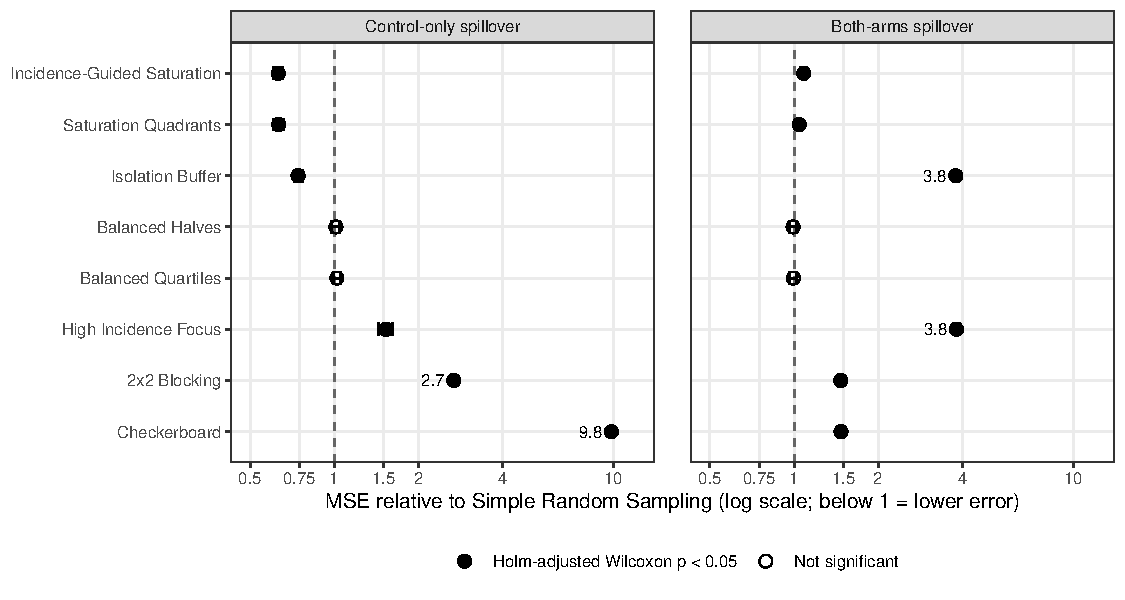
\includegraphics[width=\linewidth]{../figures/fig_vs_srs_by_regime_queen.pdf}
\caption{Each design's mean squared error (MSE) compared with simple random sampling (SRS) at $\tau = 1$ under queen contiguity, within each spillover regime. Each point is one plus the mean paired difference in MSE over the 50 independent configuration-by-surface units divided by SRS's mean MSE in that regime, so that 1 marks equal error and values below 1 mark lower error than SRS, with its $t_{49}$ 95\% interval. Filled points are significant after Holm's adjustment over the eight designs compared with SRS within the regime (Wilcoxon signed-rank test). The horizontal axis is logarithmic, ratios above 2 are printed, and rows are sorted by the control-only ratio.}
\label{fig:vs-srs}
\end{figure}

\begin{table}[!htb]

\small
\centering

\caption{Full grid benchmark at $\tau=1$, queen contiguity. Each regime-specific entry averages 80 scenarios (five incidence configurations, four $\rho$ and four $\gamma$ values). MSE is the mean squared error of the estimate of $\tau$; coverage is the proportion of 95\% $t$-based confidence intervals, with a degrees-of-freedom-corrected standard error, that contain $\tau$. Both use the oracle fit, the spatial lag model that includes the true spillover term. Simple random sampling is complete randomization of 50 clusters. No value pools queen and rook.}
\label{tab:grid-srs}
% SOURCE: results/sim_data/sim_results_MLE_tau_sweep_combined_20260927_000502.rds

\begin{tabular}{lrrrr}

\toprule
& \multicolumn{2}{c}{Both arms} & \multicolumn{2}{c}{Control only} \\
Design & MSE & Coverage & MSE & Coverage \\

\midrule
Checkerboard & 0.0624 & 0.948 & 2.1114 & 0.951 \\
High Incidence Focus & 0.1617 & 0.950 & 0.3292 & 0.945 \\
Saturation Quadrants & 0.0442 & 0.952 & 0.1359 & 0.940 \\
Isolation Buffer & 0.1608 & 0.948 & 0.1595 & 0.950 \\
$2\times2$ Blocking & 0.0623 & 0.947 & 0.5761 & 0.950 \\
Balanced Quartiles & 0.0421 & 0.949 & 0.2195 & 0.942 \\
Balanced Halves & 0.0420 & 0.949 & 0.2179 & 0.943 \\
Incidence-Guided Saturation & 0.0459 & 0.949 & 0.1355 & 0.945 \\
Simple Random Sampling & 0.0424 & 0.950 & 0.2146 & 0.946 \\

\bottomrule

\end{tabular}

\end{table}

To assess allocation risk, we additionally conducted a focused grid
pilot with queen weights, \(\tau=1\), two fixed surfaces from each incidence configuration and the extreme combinations of $\rho$ and $\gamma$, $\rho\in\{0,0.5\}$ and $\gamma\in\{0.5,0.8\}$. For assignment $a$, its risk is the conditional MSE $m(a)=E_\epsilon[(\hat\tau-\tau)^2\mid a,X]$. We estimated it by simulating repeated outcomes for each sampled assignment and then compared its distribution across assignments. This is different from the distribution
of squared errors in a single allocation or MSE across parameter
scenarios. The pilot used 100 assignment draws for each randomized design and 100 simulated outcomes per distinct assignment, and selected settings were refined to 400 outcomes on the same assignments; a design with only one possible assignment received its own outcome replication.

Averaged over the 40 units per regime in the pilot (fixed surfaces crossed with the extreme combinations of $\rho$ and $\gamma$), Incidence-Guided Saturation's control-only mean MSE is 0.1409 against SRS 0.2172, the estimated 90th percentile of allocation-specific MSE is 0.1747 against 0.2980, and the estimated worst-decile mean is 0.1936 against 0.3486. Under both arms, the
corresponding mean MSE is 0.0458 against 0.0428 and worst-decile mean
0.0582 against 0.0544. Saturation Quadrants also performs favorably under
control-only spillover; Table \ref{tab:downside} in the application section compares every design with SRS on both criteria. These selected-unit results support a qualified
downside argument for saturation; they are not the full-study grid
estimates. The focused refinement preserves the control-only direction
but reveals substantial outcome-noise contributions to estimated
allocation variation, especially under both arms. Quantiles and worst-decile membership estimated from a finite number of outcomes remain uncertain. We therefore use
the completed NC application below as the next setting-specific
assessment rather than extrapolate exact tail protection from this
pilot.

\section{Observed-incidence application: full methods and
results}\label{observed-incidence-application-full-methods-and-results}

\subsection{Purpose and observed
inputs}\label{purpose-and-observed-inputs}

The application asks which allocation designs estimate a known
education-intervention effect accurately on this geography, when some
designs use historical SUD incidence to direct treatment. It supports
planning an education intervention for healthcare professionals involved
in SUD prevention. There are no observed intervention outcomes and no
estimated relationship between local SUD incidence and education
ability. Any eventual effect on SUD incidence requires a separate
clinical evaluation. A real pilot might realize only one allocation per
planning year, making both average estimation error and poor-allocation
downside relevant.

The assignment units are 58 community college service-area clusters that
partition North Carolina's 100 counties under the study mapping (Figure
\ref{fig:service-areas}). Northampton is assigned to Halifax Community
College, Bertie to Martin Community College, and Hertford alone to
Roanoke-Chowan Community College; these are analysis conventions, not
exclusive service commitments. Observed county-year deaths and population estimates for ages 18--64 from the Surveillance, Epidemiology, and End Results program were aggregated to the same named clusters for
each year, 2018--2021. SUD deaths were identified from death
certificates with the case-adjudication algorithm of Gan and colleagues
\citep{gan_factors_2019}. The corrected numerator supplied by Habib
includes heart-failure deaths formerly excluded as presumed non-sudden.
It totals 23,523
deaths over 25,594,321 person-years. The earlier numerator reproduces
the totals behind Habib's unpublished report
\citep{habib_temporal_2026}; the corrected numerator is the application
input. We do not infer undocumented upstream exclusion rules or zip-code
allocation from the received county panel.

Annual incidence is \(100,000D_{iy}/P_{iy}\), and pooled incidence is
\(100,000\sum_yD_{iy}/\sum_yP_{iy}\), with the latter population sum
interpreted as person-years. All 58 clusters are present in each year,
and counts and populations sum back to statewide totals. We hold these
observed annual surfaces fixed, generate no synthetic incidence surface
and report years separately (Figure \ref{fig:nc-observed}). The county death-certificate source data are restricted and not publicly available; only 58-cluster summaries are reported.

\begin{figure}[!htb]

\centering
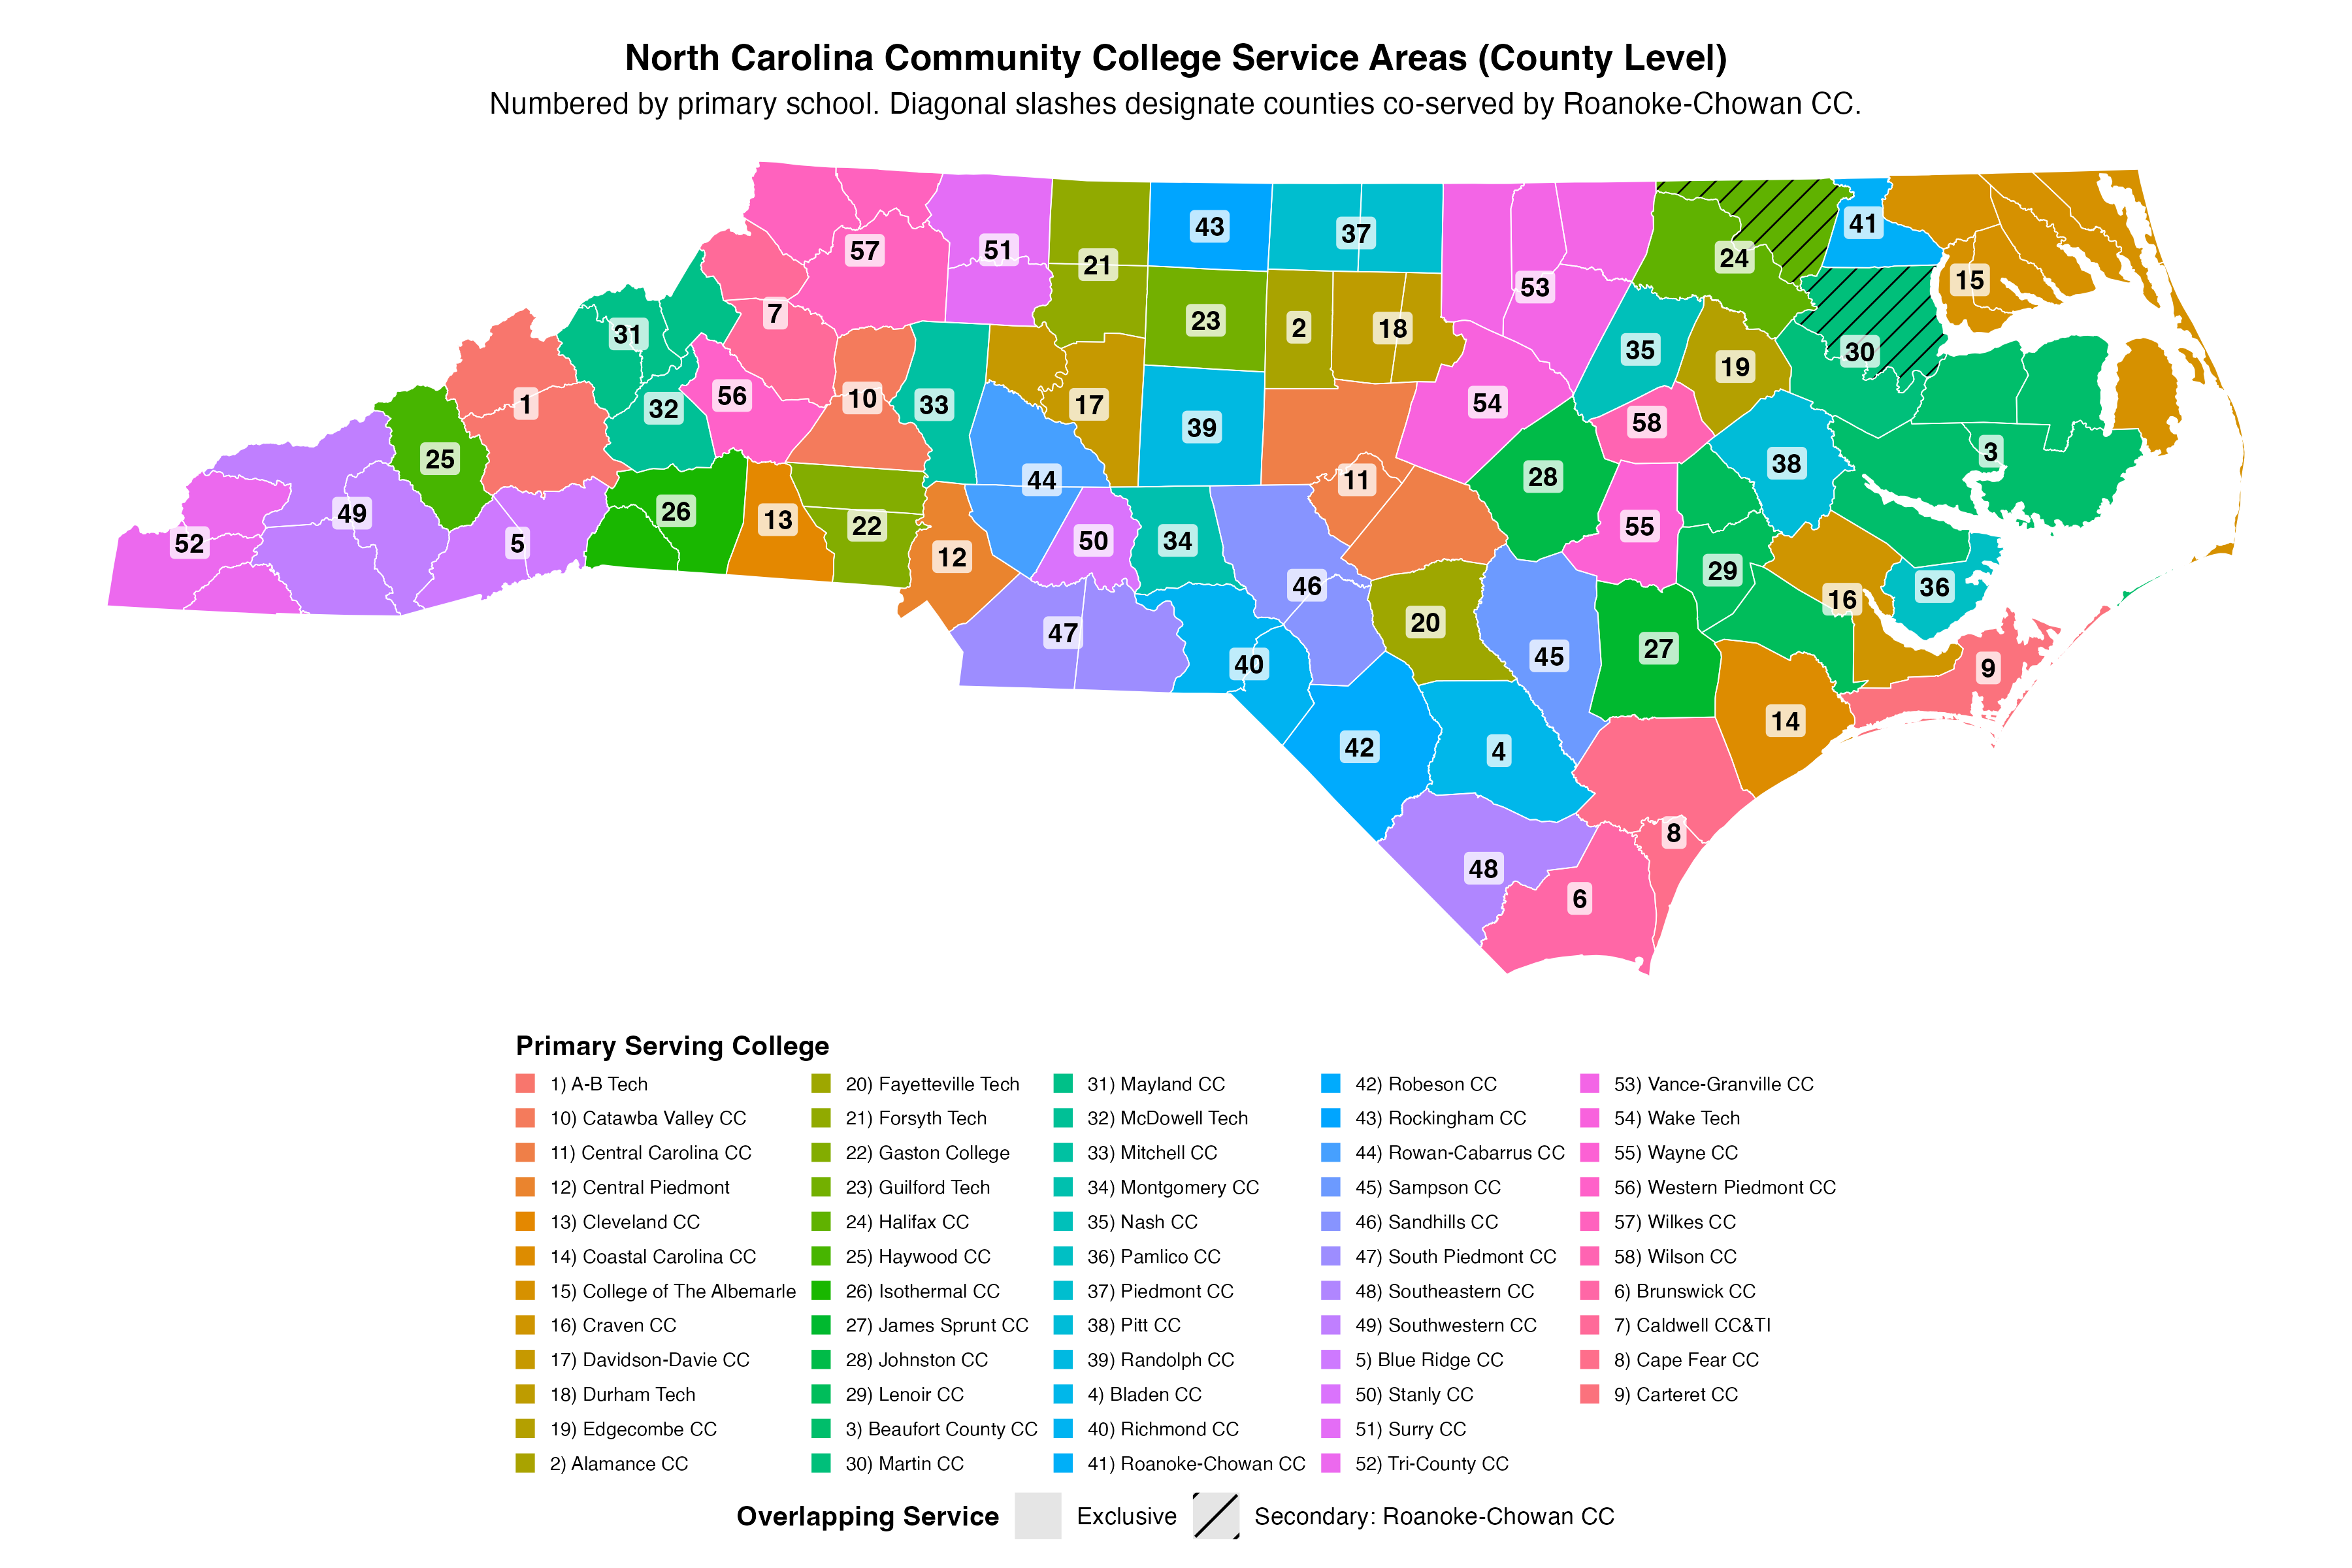
\includegraphics[width=\linewidth]{../figures/community_college_service_area_clusters.png}

\caption{The assignment of North Carolina's 100 counties to the 58 community college service areas used as clusters in the planned application. Each county is colored by its primary serving college, and each service area carries a single number, keyed to the legend. Hatching marks the two counties that also lie within Roanoke-Chowan Community College's broader service network: Northampton County, assigned to Halifax Community College (24), and Bertie County, assigned to Martin Community College (30). Roanoke-Chowan Community College (41) serves Hertford County alone in this analysis. The map shows county boundaries and the county-to-college assignment only; it does not depend on the SUD data.}
\label{fig:service-areas}

\end{figure}

\begin{figure}[!htb]

\centering
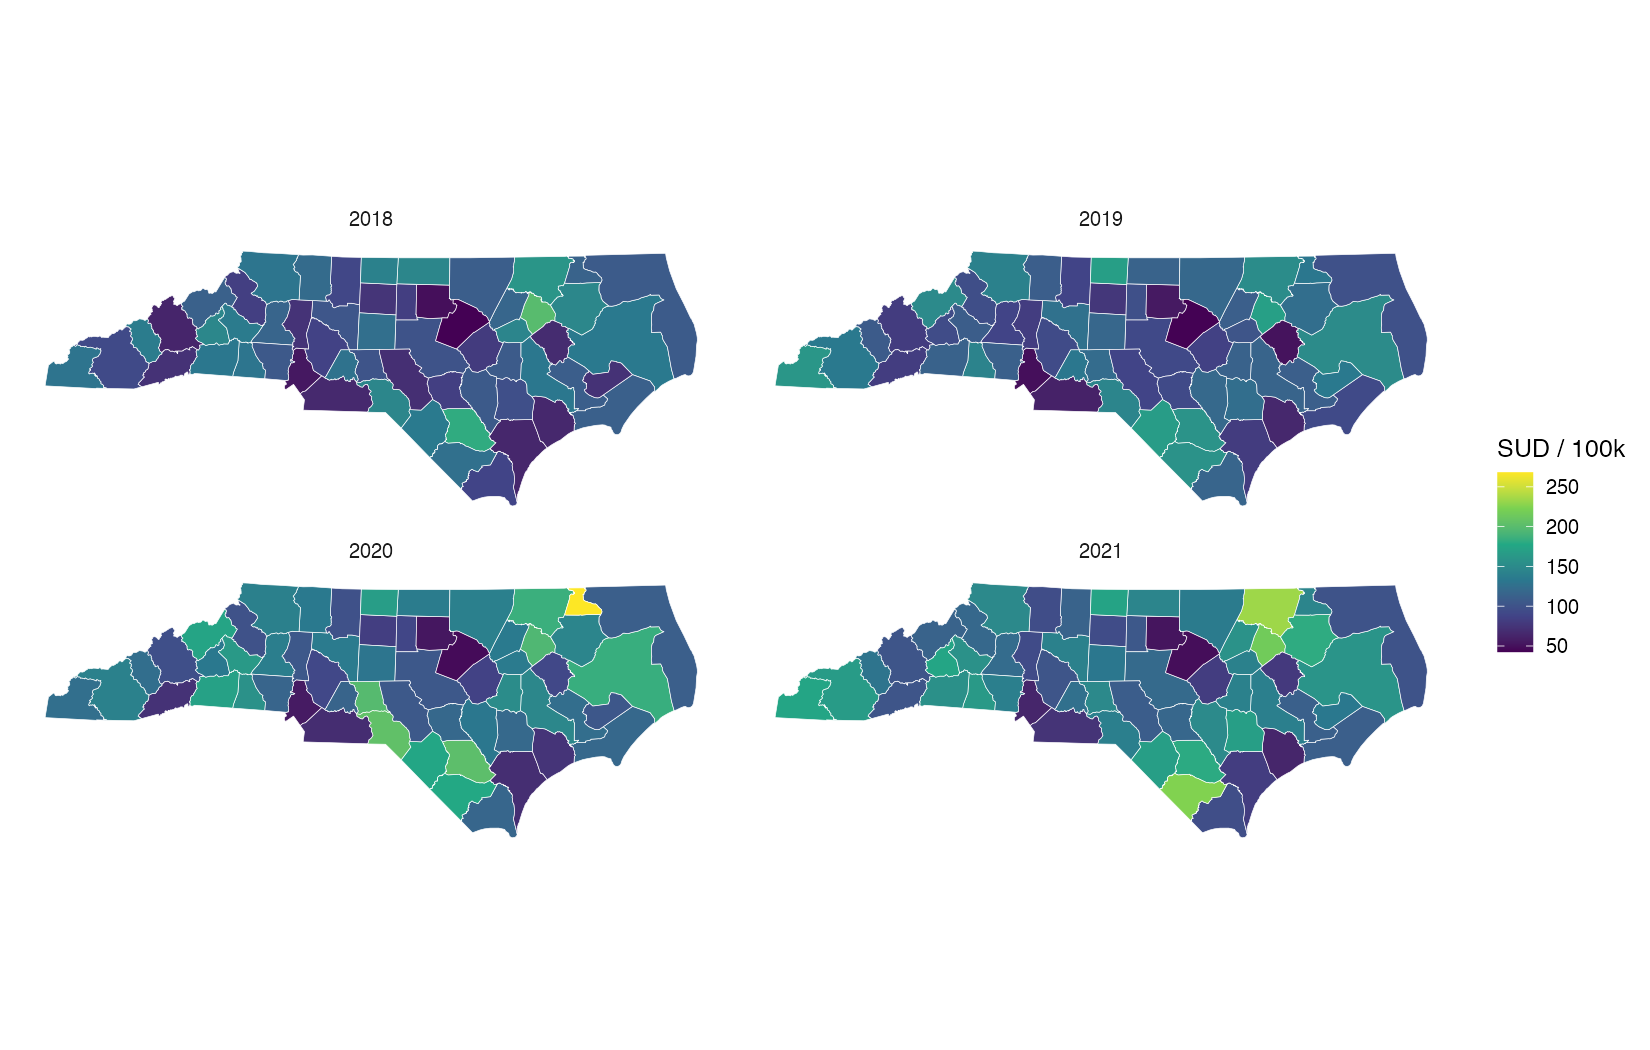
\includegraphics[width=\linewidth]{../figures/real_sud/observed_years.png}

\caption{Observed annual SUD incidence per 100,000 adults aged 18--64 in the 58 service-area clusters. These four fixed planning inputs direct incidence-aware allocation; they are not simulated outcomes or measures of education ability.}
\label{fig:nc-observed}

\end{figure}

\subsection{Geographic adaptations and treatment
budgets}\label{geographic-adaptations-and-treatment-budgets}

Queen contiguity between service areas, computed from legal county boundaries, defines primary adjacency, and rook contiguity is a sensitivity analysis. Before simulation, we checked the 58-cluster row-standardized contiguity matrix $W$, its binary adjacency and its row order against the boundary geometry. Shared legal boundaries across water can
create adjacency; this is a prespecified geographic exposure proxy, not
a measured professional communication network.

All eight designs and SRS are evaluated under the names used on the grid, adapted to the map as follows. On the NC map, Checkerboard becomes a deterministic greedy graph-coloring assignment: visit clusters by decreasing
degree, choose the arm that conflicts least with assigned neighbors,
break equal conflicts toward control, and complement the assignment if
more than half are treated. This is an interspersion analog, not a
literal rectangular checkerboard or an exact bipartite coloring. High
Incidence Focus treats the 29 highest annual-rate clusters. Isolation
Buffer draws a greedy random maximal independent set on the NC adjacency graph. SRS treats a random 29 of 58 clusters. Balanced Quartiles and
Balanced Halves stratify annual rate ranks and treat 29 overall;
odd-size strata receive their necessary extra treatments at random. In
Balanced Halves, one half receives 14 treatments and the other 15, with
the extra-treatment half chosen randomly.

The two saturation designs use one fixed four-region partition for all
years. A geographic $k$-means procedure generates 250 candidates, selecting the partition by compactness and balance in
reference population, cluster count and county count, without consulting
outcomes. Reference population is pooled person-years divided by four.
Saturation Quadrants randomly assigns 20/40/60/80\% to these regions each
draw. Incidence-Guided Saturation first ranks clusters by annual per-capita rates,
averages their ranks equally within each region, ranks those four means,
and assigns 80/60/40/20\% from highest to lowest. Regional ties are
broken randomly per allocation. Local treatment counts are rounded under
the retained design rules. Per-capita cluster rates already account for
population size; regional mean ranks answer an equally weighted cluster
question, whereas pooled regional deaths/population weights larger
clusters more heavily. Mean raw rates and pooled regional rates are
evaluated as prespecified sensitivities rather than chosen by
performance. The grid rule averages \(X\) directly: mean ranks align with its rank-scaled Poisson cases but are a deliberate application adaptation, rather than the exact rule for continuous grid incidence.

On the NC map, $2\times2$ Blocking uses spatial blocks of nearby clusters: 14 irregular groups, formed once per year by \(k\)-means on standardized
projected coordinates, incidence ranks and log(1+population), then held fixed. Half of each group, rounded, is treated randomly. This is not a
set of literal square blocks. In each year one single-cluster group remains control, because half of one cluster rounds to zero. Treatment budgets (numbers of treated clusters) differ across designs; we report them rather than modify the designs to force equal budgets (Table \ref{tab:nc-budgets}). Section \ref{app:nc} maps the
fixed regions and example assignments.

\begin{table}[!htb]
\small
\centering

\caption{Primary queen application treatment budgets. Entries are mean treated-cluster counts / percent of annual population aged 18--64. Counts and population shares use the same sampled assignments; population shares are recalculated for each year, including for designs whose assignments do not depend on annual incidence. Shares are geographic reach, not healthcare-professional enrollment.}
\label{tab:nc-budgets}
% SOURCE: application/results/real_sud_rev_20261002/exhibits/yearly_primary_design_means.csv (both-arms rows; allocation rules unchanged by regime)

\begin{tabular}{p{4.1cm}rrrr}
\toprule
Design & 2018 & 2019 & 2020 & 2021 \\
\midrule
Checkerboard & 27.00 / 50.4 & 27.00 / 50.4 & 27.00 / 50.4 & 27.00 / 50.7 \\
High Incidence Focus & 29.00 / 22.2 & 29.00 / 23.5 & 29.00 / 23.3 & 29.00 / 22.4 \\
Saturation Quadrants & 29.03 / 49.2 & 29.03 / 49.2 & 29.03 / 49.1 & 29.03 / 49.1 \\
Isolation Buffer & 15.89 / 26.7 & 15.89 / 26.7 & 15.89 / 26.7 & 15.89 / 26.7 \\
$2\times2$ Blocking & 28.00 / 50.0 & 31.00 / 55.1 & 27.00 / 48.0 & 29.00 / 50.3 \\
Balanced Quartiles & 29.00 / 48.5 & 29.00 / 49.7 & 29.00 / 50.6 & 29.00 / 49.8 \\
Balanced Halves & 29.00 / 50.0 & 29.00 / 50.5 & 29.00 / 49.2 & 29.00 / 49.4 \\
Incidence-Guided Saturation & 29.00 / 53.2 & 29.00 / 45.1 & 29.00 / 47.9 & 29.00 / 51.8 \\
Simple Random Sampling & 29.00 / 49.5 & 29.00 / 49.5 & 29.00 / 49.5 & 29.00 / 49.5 \\

\bottomrule
\end{tabular}
\end{table}

\subsection{Outcome model and Monte Carlo
evaluation}\label{outcome-model-and-monte-carlo-evaluation}

For the primary education outcome, we set \(\beta=0\) in Equation
\ref{eq:outcome}, use the 58-cluster \(W\), and fix \(\tau=1\),
\(\sigma=1\): \begin{equation}
Y=(I-\rho W)^{-1}[\tau Z+S(Z)+\epsilon],\qquad \epsilon\sim N(0,I).
\label{eq:nc-education}
\end{equation} Observed incidence affects assignments but neither
baseline education nor the constant structural intervention effect. We estimate $\tau$ with the same validated maximum likelihood implementation as in the grid study, with an intercept, \(Z\)
and the true regime-specific \(S(Z)\), without \(X\). As in the grid
model, \(\tau\) is the coefficient before spatial propagation, not an
average total impact after applying \((I-\rho W)^{-1}\). For the main application and for the analyses of partial participation and sample size below, we report $\hat\tau \pm t_{0.975,\,n-p}\,\widehat{\mathrm{SE}}\sqrt{n/(n-p)}$, where $n$ is the number of participating colleges and $p$ the number of fitted coefficients plus $\rho$, and we test $\tau = 0$ against the same $t$ distribution. The maximum likelihood variance divides by $n$, and the normal reference distribution ignores the estimated parameters. With 58 or fewer clusters, both make the Wald interval too narrow.

Primary queen settings cross \(\rho=0,0.2,0.5\), \(\gamma=0.5,0.8\),
both regimes, four years and nine designs (432 reported settings). A
matched hypothetical baseline sensitivity adds
\(X=(\operatorname{rank}_{\rm average}(rate)-0.5)/58\) with \(\beta=1\)
to both the outcome baseline and the fitted covariates (432 settings). It
changes baseline and adjustment together and is not an empirical
incidence--education association. A rook-contiguity sensitivity analysis of the primary model uses the extreme values $\rho=0,0.5$ (288 settings), and the two alternative regional summaries add 96 Incidence-Guided Saturation settings. The full application reports 1,248 settings, computed from 936 distinct simulation settings, because reported settings with the same allocations and outcome model share one simulation.

We initially sampled $J=100$ assignments and simulated $R=100$ independent outcomes per distinct assignment. A design whose set of possible assignments contains only one assignment instead received $R=1,000$ outcomes for that assignment, rather than 100 repeated copies of it counted as separate allocations. An adaptive, prespecified replication schedule extended allocations or outcomes until the Monte Carlo standard error of mean MSE was at most 5\% of mean MSE and that of coverage at most 0.01. Two single-assignment settings in the matched sensitivity analysis required $R=2,000$; all randomized designs met these targets at $J=100$ and $R=100$. Each random draw used a fixed, reproducible seed. Settings with the same set of possible assignments shared their simulations, with annual treatment counts and population shares recalculated. In the primary model, Checkerboard, Saturation Quadrants, Isolation Buffer and SRS reuse the same simulations across years, because annual incidence enters neither their allocation nor the outcome model. These repeated values are not independent
annual confirmation.

For each allocation $a$, the repeated outcomes estimate the conditional MSE \(m(a)=E_\epsilon[(\hat\tau-\tau)^2\mid a,\text{observed inputs}]\). We report its distribution across sampled allocations, its estimated 90th percentile and the estimated mean among the worst 10\% of sampled allocations, alongside unconditional mean MSE, bias and coverage. An allocation drawn more than once keeps its sampled frequency but uses one conditional estimate, and the Monte Carlo uncertainty accounts for the resulting covariance. A separate tail refinement at queen $\rho=0,0.5$, $\gamma=0.8$, both regimes and all years and designs kept the same allocations and extended the randomized designs to $R=400$ outcomes per allocation, keeping $R=1,000$ for single-assignment designs. Worst-decile assignments were identified with one half of the simulated outcomes and evaluated with the other half, to avoid selection bias. The refinement is not a new allocation sample. The rank of the fitted design matrix, residual treatment information, aliased columns, warnings, invalid estimates or intervals, and estimates of $\rho$ at the boundary of its parameter space were recorded. Section
\ref{app:nc} gives the reproducibility and precision details.

\subsection{Partial participation and sample size}

All 58 colleges will be invited to take part after the pilot, but not every college will join. We therefore repeated the application for subsets of $N$ participating colleges, $N \in \{15, 20, 25, 29, 30, 35, 40, 45, 50, 58\}$, under the education outcome model with $\beta = 0$. Under random volunteering, 50 subsets were drawn for each $N$ and shared by every design and year, so designs are compared on the same participants. In a sensitivity analysis at $N = 20$ and $N = 29$, a college's chance of joining rose linearly with its incidence rank, so that the highest-burden college was three times as likely to join as the lowest. Each design was rebuilt on the participants with its own rule, and the four saturation regions were required to contain at least two colleges each. Spatial dependence links participating colleges only, so a participant with no participating neighbor has a zero row in the participants' weights matrix $W_P$. Spillover exposure counts treated participating neighbors over all geographic neighbors, $e_j(Z) = \sum_{k \in \mathcal{N}(j)} Z_k / |\mathcal{N}(j)|$, so a non-participating neighbor counts as untreated. Spillover scales with the effect, $\gamma = \kappa\tau$ with $\kappa \in \{0.5, 0.8\}$, and the effect $\tau$ took nine values from 0 to 2 in units of the college-level outcome standard deviation. Settings crossed these with $\rho \in \{0, 0.5\}$, both spillover regimes, the nine strategies and the four planning years. With fewer than 58 participants, each setting used 20 allocations and 10 outcomes on each of the 50 subsets (10,000 fits), and a design with a single possible allocation on a subset used 200 outcomes instead. With all 58 colleges, each setting used 100 allocations and 100 outcomes, as in the main application, and it reproduced the main application's MSE and coverage within Monte Carlo error. All effect sizes share the same subsets, allocations and noise, so power curves are smooth in $\tau$. For each setting we estimated power with the corrected $t$ test above, the number of colleges needed for 80\% power, and the smallest effect detectable with 80\% power at each $N$.

The trial outcome is a score measured on each trained professional and averaged within each college. We write a professional's score as a college effect plus individual variation, with total variance 1, so that effects are in individual standard-deviation units. The intraclass correlation coefficient (ICC) is the share of that variance that lies between colleges, so the between-college variance is the ICC and the within-college variance is $1 - \text{ICC}$. Averaging the scores of $m$ professionals leaves the college part unchanged and divides the individual part by $m$, so the college mean has standard deviation $\sigma_c = \sqrt{\text{ICC} + (1 - \text{ICC})/m}$ \citep{donner_design_2000, hayes_cluster_2017}. A college-level effect of $\tau$ standard deviations is therefore an individual-level standardized effect $d = \tau\sigma_c$. With $\beta = 0$, multiplying the effect and the noise by the same constant leaves $\hat\tau/\widehat{\mathrm{SE}}$ unchanged, so power for any $m$, ICC and $d$ follows from the simulated college-level results. Rerunning one setting with the effect and the noise both halved reproduced its estimates to within $6\times10^{-8}$. In a sensitivity analysis, the number of trained professionals grew with college population ($m$ averaging 25 over participants, ICC $= 0.05$), so the noise variance differed between colleges while the fitted model stayed unweighted, as an analyst unaware of the difference would fit it.

\subsection{Further sensitivity analyses}

We compared the nine strategies with the Friedman, Nemenyi and Holm-adjusted Wilcoxon tests used on the grid, treating the 24 combinations of year, $\rho$ and $\gamma$ as blocks, separately for each spillover regime and each value of $\beta$. The four years share one map and the strategies whose allocations ignore annual incidence share their simulations across years, so these $p$-values summarize consistency rather than independent evidence.

To check that the design comparison does not depend on the spatial model, we generated data at $N = 58$ with $\beta = 0$ from the spatial lag model and fitted them by a conditional autoregressive (CAR) model \citep{besag_spatial_1974, cressie_statistics_1993} as well as by the spatial lag model. In the reverse direction, we generated data from a CAR model with the same mean and fitted them by both models. We also fitted two Bayesian models to the spatial lag data, a CAR model with the prior of Leroux and colleagues \citep{leroux_estimation_2000, lee_carbayes_2013} and a Bayesian spatial lag model \citep{lesage_introduction_2009}. Section \ref{app:nc-ext} gives the four models, their priors, the Markov chain Monte Carlo settings and the convergence checks. Finally, we replaced the proportional spillover exposure by a binary indicator of any treated neighbor and by a count of treated neighbors scaled by the mean number of neighbors, with the same form in the outcome model and the fit.

\subsection{Completed results: accuracy, inference and
reach}\label{completed-results-accuracy-inference-and-reach}

The main run generated 7,598,000 independent outcome fits. Every setting is complete and meets its prespecified precision targets for mean MSE and coverage: the largest relative Monte Carlo standard error of mean MSE is 0.04871 and the largest Monte Carlo standard error of coverage is 0.00892. There are no warnings, aliased columns, estimates of $\rho$ at the boundary of its parameter space or estimation failures. The tail refinement adds 2,280,000 independent outcomes; counting the outcomes reused from the main run only once gives 9,878,000 distinct outcomes across the two stages. Monte Carlo precision describes
uncertainty in simulated performance; it does not certify interval
calibration.

Figure \ref{fig:nc-mse} compares the eight designs with SRS by year and regime.
Under control-only spillover, Saturation Quadrants has descriptive mean MSE
0.22329 against SRS 0.30761, a 27.4\% reduction. Incidence-Guided Saturation
reduces mean MSE by 21.1--29.9\% across the four observed years (Table
\ref{tab:nc-year}). Both saturation designs have lower mean MSE than SRS in every primary parameter setting, and approximate Monte Carlo intervals for each setting-specific difference excluded zero. Neither is uniquely best: the two performed similarly, so incidence guidance lets a trial direct its highest treatment saturations to the highest-incidence regions with little or no loss of estimation accuracy, and their advantage over SRS comes from the saturation structure both designs share. High Incidence Focus is year-sensitive
under control-only spillover and cannot be recommended uniformly.

Under both-arms spillover, SRS mean MSE is 0.07638, Saturation Quadrants
0.07518, and Incidence-Guided Saturation ranges from 0.07428 to 0.07682 across
years. SRS remains competitive with balancing, blocking and saturation.
Small point differences do not establish equivalence or universal
optimality. High Incidence Focus has low both-arms MSE in the primary
model, but its allocation is deterministic for these fixed rates; this
is conditional model-based accuracy, not evidence of randomization-based
causal validity.

Mean coverage of the 95\% intervals across the four years was between 94.1\% and 94.9\% for every design and regime, and between 94.1\% and 95.1\% in single years. The Wald interval covered only 92.6\% to 93.6\% (Table \ref{tab:interval-comparison}). Meeting the Monte Carlo precision targets did not repair that finite-sample undercoverage, but the corrected $t$ interval described under Outcome model and Monte Carlo evaluation did (Section \ref{app:nc-ext}). The full year/design/regime bias and coverage table is in Section \ref{app:nc}. Checkerboard's treatment effect is identified on this irregular graph, but weak treatment--spillover separation makes its estimates imprecise; this differs from exact rook non-identification on the rectangular grid.

Population shares contextualize performance. High Incidence Focus treats
29 clusters but only about 22--24\% of working-age population, while Isolation Buffer treats a mean of 15.89 clusters and about 27\%. These population
denominators measure geographic reach, not the number of healthcare
professionals educated, intervention cost or participant-level
precision. $2\times2$ Blocking treatment counts are 28/31/27/29 by year;
complete budgets and shares are reported in Table \ref{tab:nc-budgets}
and the appendix.

Incidence-Guided Saturation sends more treatment to high-incidence regions when incidence differs between regions. On the NC map it differs little, because the four regions' mean incidence ranks lie between 24 and 34 of 58 in every year. On average, Incidence-Guided Saturation treats colleges holding 51.1\% of the summed college incidence rates, against 50.4\% for Saturation Quadrants and 62.2\% for High Incidence Focus. Shares of deaths run the other way (49.2\%, 49.6\% and 35.4\%), because the highest-rate colleges serve small populations. On the simulation grid, where regional incidence differed more, incidence guidance raised the treated share of incidence by 2.1 to 3.1 percentage points over Saturation Quadrants, and across surfaces the gain rose with the spread of the regions' mean incidence ranks (correlation 0.84 to 0.99; Figure \ref{fig:spread-gain} in Section \ref{app:nc-ext}).

\begin{figure}[!htb]
\centering
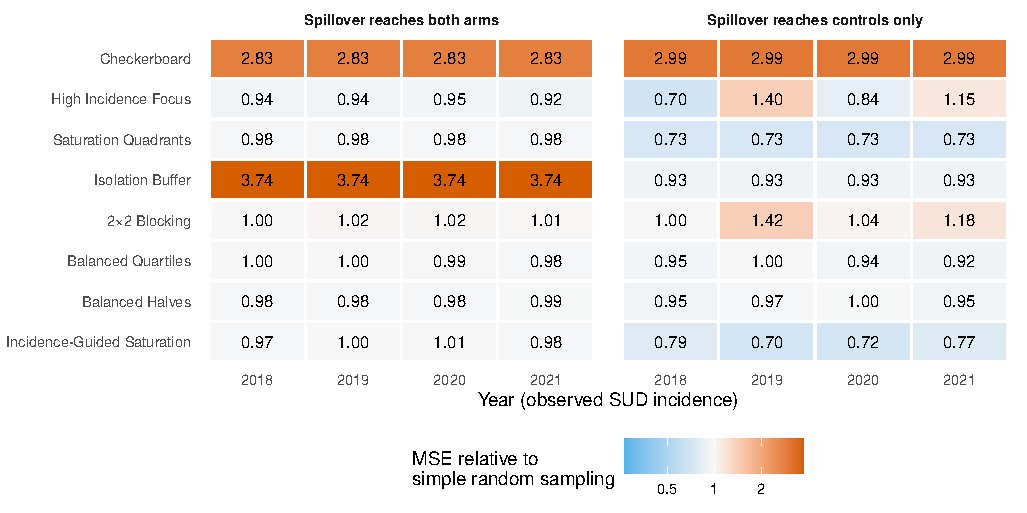
\includegraphics[width=\linewidth]{../figures/compact/nc_annual_accuracy.pdf}
\caption{Completed primary application: yearly mean MSE divided by year- and regime-matched SRS MSE, for the eight other designs with queen weights and education outcomes. Each cell averages six $\rho/\gamma$ settings equally before taking the ratio. Blue indicates lower error than SRS, orange higher error; colors use a logarithmic ratio scale and cells print the ratios. SRS mean MSE is 0.07638 under both arms and 0.30761 control-only. Years that share the same simulations are not independent replications. Absolute MSE, bias, coverage, budgets and setting-specific comparisons are in Section \ref{app:nc}.}
\label{fig:nc-mse}
\end{figure}

\begin{table}[!htb]
\small
\centering

\caption{Primary application yearly mean MSE, queen contiguity; equal weights over the six $\rho/\gamma$ pairs. Saturation Quadrants and SRS reuse the same simulations across years.}
\label{tab:nc-year}
% SOURCE: application/results/real_sud_rev_20261002/exhibits/yearly_primary_design_means.csv

\begin{tabular}{lrrrrr}
\toprule
& \multicolumn{2}{c}{Both arms} & \multicolumn{3}{c}{Control only} \\
Year & SRS & \shortstack{Incidence-Guided\\Saturation} & SRS & \shortstack{Saturation\\Quadrants} & \shortstack{Incidence-Guided\\Saturation} \\
\midrule
2018 & 0.07638 & 0.07428 & 0.30761 & 0.22329 & 0.24285 \\
2019 & 0.07638 & 0.07628 & 0.30761 & 0.22329 & 0.21565 \\
2020 & 0.07638 & 0.07682 & 0.30761 & 0.22329 & 0.22029 \\
2021 & 0.07638 & 0.07450 & 0.30761 & 0.22329 & 0.23732 \\

\bottomrule
\end{tabular}
\end{table}

\subsection{Allocation downside and
sensitivity}\label{allocation-downside-and-sensitivity}

At the two refined queen settings, $\rho=0$ and $\rho=0.5$ with $\gamma=0.8$, under control-only spillover, Saturation Quadrants' estimated 90th percentile of allocation-specific MSE is 31.8--32.9\%
below SRS and its estimated worst-decile mean 34.6--37.8\% below. Incidence-Guided
Saturation's corresponding reductions are 20.8--38.6\% and 20.7--43.4\%.
The pattern persists when worst-decile assignments are identified with one half of the simulated outcomes and evaluated with the other half, which avoids selection bias. Figure \ref{fig:nc-risk} shows the $\rho=0.5$ setting. This supports a descriptive downside benefit
alongside lower average error, conditional on the studied model and
sampled assignments.

Table \ref{tab:downside} compares every design with SRS on both criteria, mean conditional MSE and the mean of the worst 10\% of sampled allocations, in the grid pilot and at the refined NC settings. Under control-only spillover, both saturation designs had lower mean and worst-decile MSE than SRS in both settings. Isolation Buffer also had a lower worst decile than SRS under control-only spillover (0.62 of SRS in the grid pilot and 0.91 in NC), but under both-arms spillover its mean was 3.79 and 3.69 times that of SRS, and it treated fewer clusters. High Incidence Focus has a single allocation in NC. That allocation's MSE was below the SRS worst-decile mean under both regimes (0.76 under both arms and 0.64 under control-only spillover), with mean MSE close to SRS (0.93 and 1.03). In the grid pilot, however, its both-arms mean was 3.91 times that of SRS, and its NC result depends on the incidence model (next paragraph). Balanced Quartiles and Balanced Halves matched SRS on both criteria. Checkerboard and $2\times2$ Blocking did not improve on SRS on either criterion in any setting.

\begin{table}[!htb]

\footnotesize
\centering
\setlength{\tabcolsep}{4pt}

\caption{Mean conditional MSE and worst-decile mean conditional MSE of each design relative to SRS: each entry is the design's average divided by SRS's average in the same setting and spillover regime (below 1 is lower error than SRS). Grid: focused pilot, queen contiguity, $\tau=1$, averaged over 40 units, each a fixed incidence surface with one of the extreme combinations of $\rho$ and $\gamma$. NC: refined queen settings $\rho\in\{0,0.5\}$, $\gamma=0.8$, averaged with equal weight over 2018--2021 and both values of $\rho$; NC designs are the map adaptations (Checkerboard as a greedy graph-coloring assignment, $2\times2$ Blocking on spatial blocks of nearby clusters, and both saturation designs on four fixed regions). A design with one allocation has worst-decile mean equal to its mean.}
\label{tab:downside}
% SOURCE: results/allocation_risk/summary/downside_by_design.csv (code/21_downside_by_design.R)

\begin{tabular}{lrrrrrrrr}

\toprule
& \multicolumn{4}{c}{Grid pilot} & \multicolumn{4}{c}{NC application} \\
& \multicolumn{2}{c}{Both arms} & \multicolumn{2}{c}{Control only} & \multicolumn{2}{c}{Both arms} & \multicolumn{2}{c}{Control only} \\
Design & Mean & Worst 10\% & Mean & Worst 10\% & Mean & Worst 10\% & Mean & Worst 10\% \\

\midrule
Checkerboard & 1.41 & 1.10 & 9.80 & 6.11 & 2.68 & 2.20 & 3.02 & 1.88 \\
High Incidence Focus & 3.91 & 3.11 & 1.38 & 0.87 & 0.93 & 0.76 & 1.03 & 0.64 \\
Saturation Quadrants & 1.06 & 1.05 & 0.62 & 0.53 & 0.99 & 0.94 & 0.73 & 0.64 \\
Isolation Buffer & 3.79 & 3.93 & 0.75 & 0.62 & 3.69 & 4.75 & 0.93 & 0.91 \\
$2\times2$ Blocking & 1.44 & 1.57 & 2.68 & 2.63 & 1.00 & 1.02 & 1.15 & 1.18 \\
Balanced Quartiles & 0.99 & 1.00 & 1.00 & 1.00 & 0.98 & 0.96 & 0.95 & 1.01 \\
Balanced Halves & 0.99 & 1.00 & 1.00 & 0.98 & 0.98 & 0.96 & 0.97 & 0.99 \\
Incidence-Guided Saturation & 1.07 & 1.07 & 0.65 & 0.56 & 0.98 & 0.93 & 0.75 & 0.68 \\
Simple Random Sampling & 1.00 & 1.00 & 1.00 & 1.00 & 1.00 & 1.00 & 1.00 & 1.00 \\

\bottomrule

\end{tabular}

\end{table}

Figure \ref{fig:alloc-dist} shows the full allocation-to-allocation distribution for the six designs and SRS. Under control-only spillover, most Incidence-Guided Saturation allocations had lower MSE than the average SRS allocation in both studies, whereas the SRS distribution extended well above its mean.

\begin{figure}[!htb]
\centering
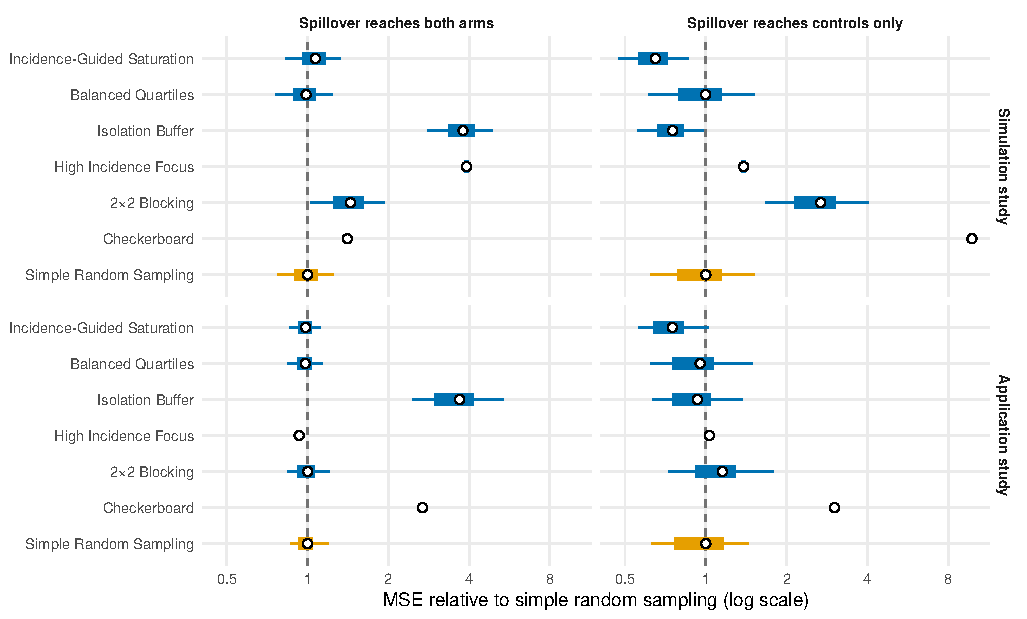
\includegraphics[width=\linewidth]{../figures/compact/allocation_distribution_by_design.pdf}
\caption{Distribution of allocation-specific MSE for the six designs and simple random sampling (SRS), relative to the mean MSE of SRS in the same setting (queen weights). Simulation study: focused grid pilot at $\tau=1$, 40 fixed surface/parameter settings per spillover regime. Application study: refined NC settings ($\rho=0, 0.5$; $\gamma=0.8$) in each year 2018--2021. For each allocation, MSE is estimated from repeated simulated outcomes (100 in the simulation study, at least 400 in the application study). Thin lines span the 5th to 95th percentiles of allocations and thick bars the 25th to 75th; circles mark the mean. Percentiles are computed within each setting and then averaged, so bars show allocation-to-allocation spread; a design with one allocation per setting appears as a circle only. Outcome Monte Carlo noise in the per-allocation estimates widens the bars slightly.}
\label{fig:alloc-dist}
\end{figure}


Tail uncertainty remains material. With \(J=100\), the worst decile
contains only ten sampled draws; extra outcomes reduce noise in
\(\hat m(a)\) but do not enlarge the allocation sample. All 112 reported settings in the tail refinement for designs with more than one possible assignment flag uncertain worst-decile membership. Under both arms, the overlap between the worst deciles identified by the two outcome halves (the Jaccard index: allocations in both divided by allocations in either) was 0--0.25 for Incidence-Guided Saturation, and approximately 61--86\% of the raw variance of estimated risk across allocations was attributable to outcome Monte Carlo noise. Saturation Quadrants' worst-decile membership was similarly unstable. Small both-arms tail differences therefore do not establish superior downside protection. Checkerboard and High Incidence Focus each have only one possible assignment for these inputs; their 90th percentile and worst-decile mean equal their conditional mean MSE, which does not imply low error or absence of outcome uncertainty.



In the matched hypothetical incidence-baseline/X-adjusted sensitivity,
High Incidence Focus MSE rises to roughly 3.68--4.44 times its primary
value under both arms and 1.42--2.52 times under control-only spillover.
Treatment--incidence alignment leaves less residual treatment
information after adjustment; this sensitivity changes baseline and
adjustment jointly and does not imply that SUD incidence predicts
education ability. Rook and queen comparisons matched at the same extreme combinations of $\rho$ and $\gamma$ preserve broad regime-specific conclusions. Alternative regional summaries change the regional ordering in some years; where an alternative summary gives the same ordering and ties, it gives the same set of possible assignments and so the same results. We retain the
prespecified mean-rank rule rather than select a summary
retrospectively. Section \ref{app:nc} reports the matched sensitivity
table and regional ordering.

\subsection{Planning for realistic participation}

Under both-arms spillover, the design hardly affected the number of colleges a trial needs. Every design except Checkerboard and Isolation Buffer needed 35 to 37 colleges for 80\% power to detect a college-level effect of one standard deviation, and about 19 colleges for 1.5 standard deviations (Figure \ref{fig:colleges-needed}, Table \ref{tab:nc-power}). Checkerboard and Isolation Buffer did not reach 80\% power at $\tau = 1$ even with all 58 colleges. Under control-only spillover, no design reached 80\% power at $\tau = 1$ with all 58 colleges. At $\tau = 1.5$ the two saturation designs needed 28 colleges, against 29 to 32 for SRS and the rank-based designs, while $2\times2$ Blocking and Isolation Buffer failed to reach 80\% power with 58 colleges in one of the four planning years. Power under control-only spillover rose slowly beyond about 40 colleges (Figure \ref{fig:power-n}). When nearly every college participates, nearly every control has a treated neighbor, so spillover exposure varies little and is hard to separate from treatment. Non-participating neighbors restore some of that variation, and so do the saturation designs. With all 58 colleges, the smallest effect detectable with 80\% power was 0.76 to 0.78 college-level standard deviations under both-arms spillover for every design except Checkerboard (1.32) and Isolation Buffer (1.50), and 1.24 to 1.25 for the two saturation designs under control-only spillover, against 1.45 to 1.57 for SRS and the rank-based designs.

\begin{figure}[!htb]
\centering
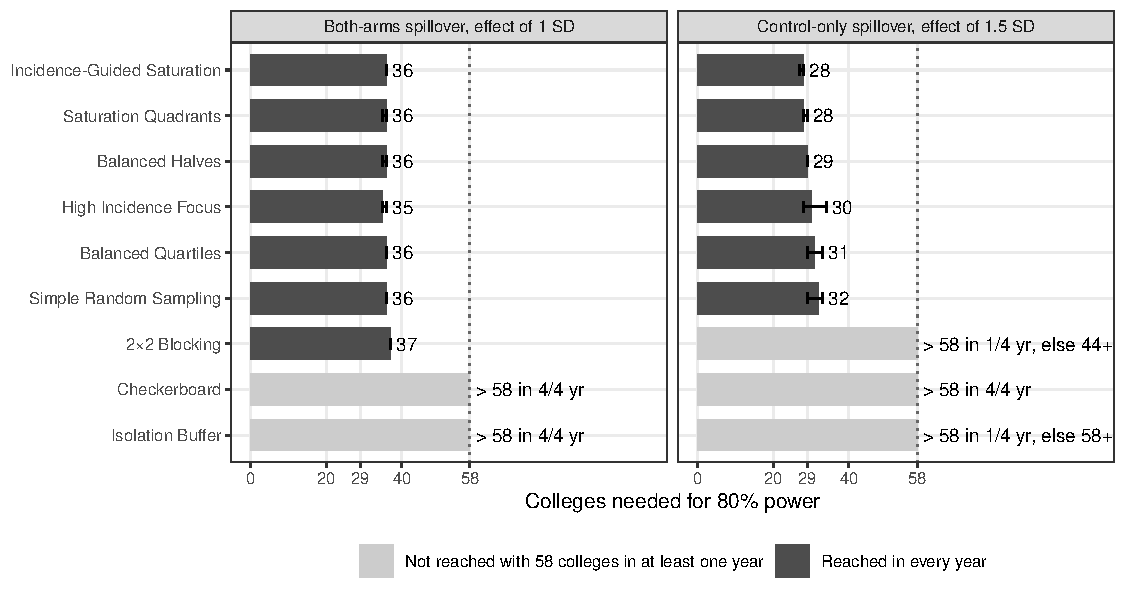
\includegraphics[width=\linewidth]{../figures/fig_colleges_needed.pdf}
\caption{Number of participating colleges needed for 80\% power with the corrected $t$ test, by design, for a college-level effect of $\tau = 1$ standard deviation under both-arms spillover and $\tau = 1.5$ under control-only spillover. Random volunteering, $\rho = 0.5$ and spillover $\gamma = 0.8\tau$. Dark bars show the mean over the 2018--2021 planning years and whiskers the range. Light bars mark designs that did not reach 80\% power with all 58 colleges in the stated number of years, with the smallest number needed in the other years.}
\label{fig:colleges-needed}
\end{figure}

\begin{figure}[!htb]
\centering
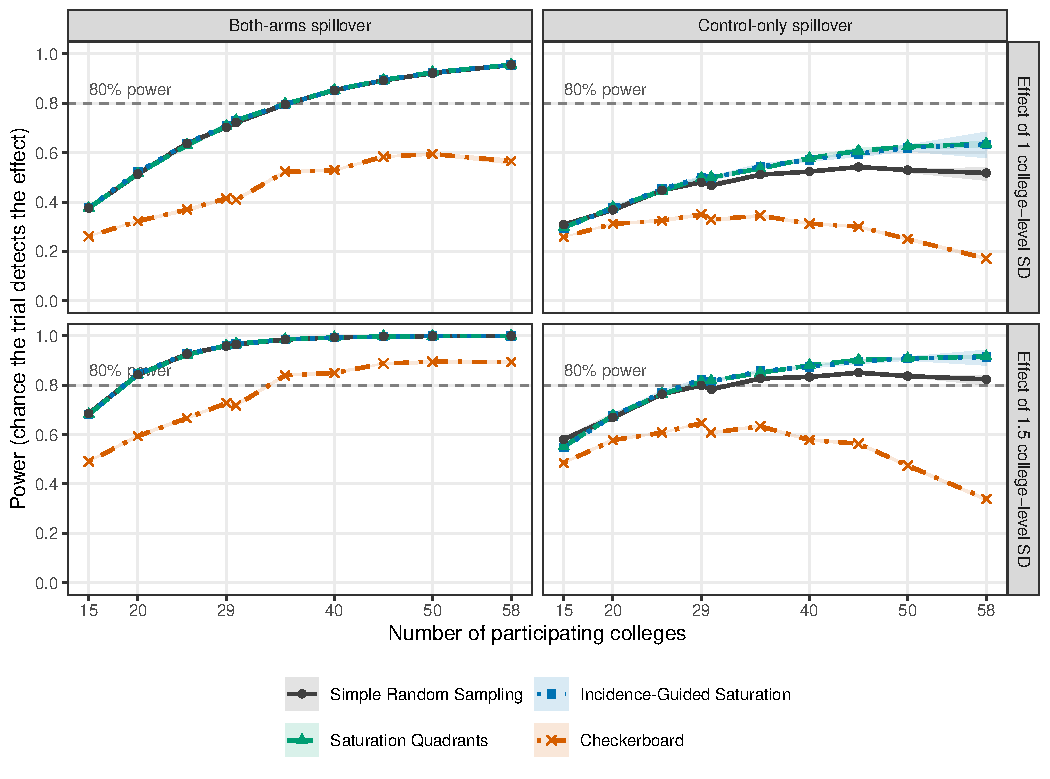
\includegraphics[width=\linewidth]{../figures/fig_power_vs_n.pdf}
\caption{Power of the corrected $t$ test against the number of participating colleges for simple random sampling (SRS), the two saturation designs and Checkerboard, by spillover regime (columns) and college-level effect (rows). Random volunteering, $\rho = 0.5$ and spillover $\gamma = 0.8\tau$. Lines show the mean over the 2018--2021 planning years and bands the range, which is narrower than the lines except near 58 colleges, and the dashed line marks 80\% power. The two saturation designs nearly coincide. Each number of colleges uses its own 50 random participant subsets, so the small drop from 29 to 30 colleges reflects which subsets were drawn.}
\label{fig:power-n}
\end{figure}

For a trial with $m = 25$ trained professionals per college and an ICC of 0.05, so that $\sigma_c = 0.30$, an individual-level effect of $d = 0.3$ gives power 0.71 to 0.72 with 29 colleges and 0.96 with 58 under both-arms spillover, for SRS and for both saturation designs. Under control-only spillover the same effect gives power 0.49 and 0.53 with SRS, and 0.51 and 0.64 with Incidence-Guided Saturation (Table \ref{tab:nc-translation} in Section \ref{app:nc-ext}). Letting the number of professionals grow with college population, at the same average of 25, reduced power by about 0.1 for every design and changed no design's relative standing.

The Wald test rejected a true null hypothesis in 11\% to 13\% of simulated trials with 15 colleges and in 6\% to 7\% with 58. With the corrected $t$ test the rejection rate was 4.4\% to 5.6\%, and the coverage of the corrected interval at $\tau = 1$ was between 94.0\% and 95.6\% for every design and regime at every number of colleges (Table \ref{tab:nc-calibration} in Section \ref{app:nc-ext}). The colleges-needed numbers above therefore come from a test with the nominal size.

The regime-specific guidance held with fewer participants, but the size of the saturation advantage depended on participation (Table \ref{tab:nc-guidance} in Section \ref{app:nc-ext}). Checkerboard and Isolation Buffer remained worse than SRS under both-arms spillover at every number of colleges, and the rank-based designs remained within a few percent of SRS. Under control-only spillover, the saturation designs' mean MSE was 22\% below that of SRS with 58 colleges, 9\% to 10\% below with 40, 4\% to 5\% below with 29 and about 1\% below with 20. With few participants, non-participating neighbors already create the exposure variation that saturation otherwise supplies. When the colleges with higher incidence were more likely to volunteer, the saturation designs' advantage over SRS was 2\% or less at 20 and 29 colleges. Isolation Buffer went from matching SRS under control-only spillover with 58 colleges to 2.3 times SRS's MSE with 29 colleges and 6.2 times with 15.

The design comparison did not depend on the spatial model used to generate or fit the data, with one exception (Section \ref{app:nc-ext}). Fitting a CAR model, generating the data from a CAR model, or both, left the saturation designs with 0.76 to 0.82 times SRS's MSE under control-only spillover, and Checkerboard and Isolation Buffer the worst designs under both-arms spillover. A Bayesian spatial lag model reproduced the maximum likelihood results, with posterior means correlated 0.999 with the maximum likelihood estimates, credible-interval coverage of 94.6\% to 95.3\% and the same design ordering. The exception is the Bayesian CAR model with strong spatial dependence ($\rho = 0.5$). Its estimates were biased by 0.14 to 0.22 even when its chains converged, its coverage was 88\% to 90\%, and it did not reproduce the saturation designs' control-only advantage. That model assumes a different dependence structure from the one that generated the data, and the correctly specified Bayesian model does not share the problem. Under a binary spillover exposure Isolation Buffer was never identified, and under a count exposure the saturation designs remained the best under control-only spillover. Formal tests over the 24 combinations of year, $\rho$ and $\gamma$ rejected equal ranks for every regime and value of $\beta$ (Friedman $\chi^2$ from 135 to 180 on 8 degrees of freedom), and under control-only spillover the two saturation designs had the two best average ranks.

The application supports considering either saturation strategy when
control-only spillover is plausible, and SRS alongside other randomized
strategies when both-arm exposure is expected. A trial team should
consider likely spillover, recruitment, cluster and participant budgets,
achievable measurement precision and interval calibration before
selecting one realized allocation. The findings do not establish
intervention effectiveness or a final trial protocol.

\section{The eight-design
comparison}\label{s1.-the-eight-design-comparison}

\applabel{S4}{app:eight-design}Table \ref{tab:excluded-designs} defines
the two related variants excluded from the detailed six-design grid
ranking but included in the main-text nine-design benchmark and
application, in the format of Table \ref{tab:designs}, and Table
\ref{tab:eight-design} reports the comparison of all eight designs at
the primary scenario, \(\tau = 1\).

\begin{table}[!htb]

\small
\centering

\caption{The two related variants outside the detailed six-design grid ranking, in the format of Table \ref{tab:designs}. Saturation Quadrants shares its mechanism with Incidence-Guided Saturation, and Balanced Halves with Balanced Quartiles (see Treatment assignment designs). A cluster's incidence rank is its rank by the baseline incidence surface $X_k$, with ties broken at random in every draw. Clusters treated is the number of clusters treated per assignment.}
\label{tab:excluded-designs}

\begin{tabular}{p{3.4cm}p{6.4cm}p{2.0cm}p{2.3cm}}

\toprule
Design & Assignment rule & Clusters treated & Deterministic \\

\midrule
Saturation Quadrants & The grid is divided into its four $5\times5$ coordinate quadrants, which are given saturations of 20\%, 40\%, 60\%, and 80\% in an order drawn at random for each assignment, without reference to incidence; within each quadrant, that share of its 25 clusters is treated at random & 50 & No \\
Balanced Halves & Clusters are divided by incidence rank into two strata of 50; 25 clusters are treated at random in each stratum & 50 & No \\

\bottomrule

\end{tabular}

\end{table}

The argument for leaving Saturation Quadrants and Balanced Halves out of
the detailed grid analysis, with the Nemenyi and Wilcoxon results for
each pair, is given under Treatment assignment designs in Methods; Table
\ref{tab:eight-design} supplies the rest of the eight-design comparison.
Under both neighbor types, each excluded design is adjacent to its
retained counterpart in mean MSE. The MSEs and coverages of the six
retained designs are those of Table \ref{tab:performance}, given here to
four and three decimal places.

\begin{table}[!htb]

\small
\centering

\caption{Performance of all eight designs and SRS at the primary scenario, $\tau = 1$, under queen contiguity (primary) and rook contiguity (sensitivity), pooled over the five incidence configurations. Each entry averages the 160 scenarios of one design and neighbor type (5 incidence configurations $\times$ 4 values of $\rho$ $\times$ 4 values of $\gamma$ $\times$ 2 spillover regimes), each summarizing 250 fits of the oracle model. Rows in both panels are in order of mean squared error (MSE) under queen contiguity. Retained marks the six designs compared in the detailed grid analysis, and SRS is the benchmark. Average rank is the mean of each design's within-block MSE rank among the eight designs and SRS over the 160 blocks (1 = lowest MSE), so it differs from the average rank in Table \ref{tab:performance}. Under rook contiguity, $\tau$ is not identified for Checkerboard; its estimates are kept and flagged.}
\label{tab:eight-design}

\begin{tabular}{lcccc}

\toprule
Design & Retained & MSE & Coverage & Average rank \\

\midrule
\multicolumn{5}{l}{\textit{Queen contiguity (primary)}} \\
Saturation Quadrants & No & 0.0900 & 0.946 & 2.394 \\
Incidence-Guided Saturation & Yes & 0.0907 & 0.947 & 2.700 \\
Simple Random Sampling & Benchmark & 0.1285 & 0.948 & 3.788 \\
Balanced Halves & No & 0.1299 & 0.946 & 3.831 \\
Balanced Quartiles & Yes & 0.1308 & 0.946 & 3.906 \\
Isolation Buffer & Yes & 0.1602 & 0.949 & 5.638 \\
High Incidence Focus & Yes & 0.2455 & 0.948 & 7.763 \\
2$\times$2 Blocking & Yes & 0.3192 & 0.948 & 7.244 \\
Checkerboard & Yes & 1.0869 & 0.950 & 7.737 \\

\midrule
\multicolumn{5}{l}{\textit{Rook contiguity (sensitivity)}} \\
Saturation Quadrants & No & 0.0708 & 0.949 & 2.587 \\
Incidence-Guided Saturation & Yes & 0.0717 & 0.952 & 2.650 \\
Simple Random Sampling & Benchmark & 0.0850 & 0.947 & 3.612 \\
Balanced Halves & No & 0.0842 & 0.949 & 3.569 \\
Balanced Quartiles & Yes & 0.0837 & 0.948 & 3.369 \\
Isolation Buffer & Yes & 0.1329 & 0.950 & 6.050 \\
High Incidence Focus & Yes & 0.2062 & 0.948 & 7.969 \\
2$\times$2 Blocking & Yes & 0.1281 & 0.948 & 6.206 \\
Checkerboard (flagged) & Yes & 0.4799 & 0.162 & 8.988 \\

\bottomrule

\end{tabular}

\end{table}

\section{Simulation mechanics}\label{s2.-simulation-mechanics}

\applabel{S5}{app:mechanics}This section gives the mechanical details
behind Simulation design, resampling, and metrics (Methods): the
parameter grid, the random-number streams, the Monte Carlo structure,
and the exact formulas for the metrics and their Monte Carlo standard
errors.

\textbf{Parameter grid.} Table \ref{tab:parameter-grid} lists the
parameters that were crossed to form the 12,800 scenarios and the
settings that were held fixed.

\begin{table}[!htb]

\small
\centering

\caption{Parameter grid of the original eight-design simulation. The crossed parameters form $5 \times 5 \times 2 \times 4 \times 4 \times 2 \times 8 = 12{,}800$ scenarios, 9,600 of them for the six designs compared in the detailed grid analysis; the settings in the lower panel are the same in every scenario.}
\label{tab:parameter-grid}

\begin{tabular}{p{5.8cm}p{7.6cm}c}

\toprule
Parameter & Values & Levels \\

\midrule
\multicolumn{3}{l}{\textit{Crossed}} \\
Treatment effect $\tau$ & 0.8, 1.0 (primary), 1.5, 2.0, 3.0 & 5 \\
Incidence configuration & iid; spatially autocorrelated, $\rho_X \in \{0.20, 0.50\}$; Poisson, $\rho_X \in \{0.20, 0.50\}$ & 5 \\
Neighbor type & Queen (primary), rook (sensitivity) & 2 \\
Outcome spatial dependence $\rho$ & 0, 0.01, 0.20, 0.50 & 4 \\
Spillover magnitude $\gamma$ & 0.5, 0.6, 0.7, 0.8 & 4 \\
Spillover regime & Both arms, control only (Equation \ref{eq:spillover}) & 2 \\
Design & The six designs of Table \ref{tab:designs} and the two of Table \ref{tab:excluded-designs} & 8 \\

\midrule
\multicolumn{3}{l}{\textit{Fixed}} \\
Grid & Regular $10\times10$ grid, $N = 100$ clusters & \\
Outcome model (Equation \ref{eq:outcome}) & $\beta = 1$, $\sigma = 1$ & \\
Poisson mechanism & Base rate 35 per 100,000; $P = 100{,}000$ per cluster & \\
Incidence surfaces per configuration & $K = 10$ & \\
Assignments per surface & $J = 25$ (Checkerboard: one assignment, used in every draw) & \\
Fits per scenario and estimator & $KJ = 250$, each with its own noise vector & \\
Estimators & Oracle (primary) and non-oracle (sensitivity), both fit to every simulated outcome & \\

\bottomrule

\end{tabular}

\end{table}

\textbf{Random-number streams.} Every random draw in the simulation has
its own seed, computed by hashing a key that names the draw. The key
lists the draw's type (incidence surface, assignments, or noise) and the
parameters that identify it, with numeric values written to a fixed
number of decimal places so that equal values always give the same key.
The random-number generator and its methods for normal and discrete
draws are also fixed explicitly, so the streams do not depend on
software defaults. Table \ref{tab:seed-keys} lists the three kinds of
draw, the parameters in their keys, and the scenarios that therefore
share them. The consequences of this scheme, independence from the order
of execution and common random numbers, are described in Methods.

\begin{table}[!htb]

\small
\centering

\caption{Seed keys. Each key names the kind of draw and the parameters listed here; the incidence mechanism is iid, spatial, or Poisson, and the iid configuration, which has no $\rho_X$, uses 0 in its place. $k$ indexes the incidence surface and $d$ the design. A draw is shared by every scenario whose key parameters match its own.}
\label{tab:seed-keys}

\begin{tabular}{p{4.2cm}p{5.0cm}p{5.2cm}}

\toprule
Draw & Key parameters & Shared by \\

\midrule
Incidence surface $X_k$ & Incidence mechanism, $\rho_X$, $k$ & Every block, design, and value of $\tau$ of the configuration \\
The $J = 25$ assignments of design $d$ on surface $k$ & Incidence mechanism, $\rho_X$, neighbor type, $\rho$, $\gamma$, spillover regime, $k$, $d$ & All five values of $\tau$ and both estimators \\
The 250 noise vectors of a block & Incidence mechanism, $\rho_X$, neighbor type, $\rho$, $\gamma$, spillover regime & All eight designs, all five values of $\tau$, and both estimators \\

\bottomrule

\end{tabular}

\end{table}

\textbf{Monte Carlo structure and checkpoints.} Within a scenario, fit
\((k, j)\), with \(k = 1, \dots, 10\) and \(j = 1, \dots, 25\), uses
surface \(X_k\), assignment \(Z_{kj}\), and noise vector
\(\epsilon_{kj}\), the \((k, j)\) column of the block's
\(100 \times 250\) noise matrix (see Simulation design, resampling, and
metrics). The unit of computation is a combination of incidence
configuration, neighbor type, and \(\rho\): 40 units, each covering 4
values of \(\gamma\), 2 spillover regimes, 8 designs, 5 values of
\(\tau\), 250 fits, and 2 estimators. The units ran in parallel, and the
run stops if any unit fails. Each unit's results are saved together with
a record of the parameter settings, the simulation code, and the
software versions that produced them, and saved results are reused only
if all of these match the current run, so results from different code or
settings are never combined.

\textbf{Scenario metrics.} For one scenario and estimator, let
\(f = 1, \dots, n\) index the valid fits, those with a finite estimate
and standard error (here every fit was valid, so \(n = 250\)). Let
\(L_f, U_f = \hat\tau_f \mp t_{0.975,\,N-p}\,\widehat{\text{SE}}_f\sqrt{N/(N-p)}\), with \(N = 100\) clusters and \(p\) as defined in the detailed methods (the Wald limits replace the multiplier by \(z_{0.975} = \Phi^{-1}(0.975) \approx 1.96\)), and let
\(\bar{\hat\tau} = n^{-1}\sum_f \hat\tau_f\). Then \[
\text{Bias} = \frac{1}{n}\sum_{f=1}^{n}(\hat\tau_f - \tau), \qquad
\text{SD} = \left\{\frac{1}{n-1}\sum_{f=1}^{n}\left(\hat\tau_f - \bar{\hat\tau}\right)^2\right\}^{1/2}, \qquad
\text{MSE} = \frac{1}{n}\sum_{f=1}^{n}(\hat\tau_f - \tau)^2,
\] \[
\text{Coverage} = \frac{1}{n}\sum_{f=1}^{n}\mathbf{1}\{L_f \le \tau \le U_f\}, \qquad
\text{Power} = \frac{1}{n}\sum_{f=1}^{n}\mathbf{1}\{L_f > 0\},
\] so that \(\text{MSE} = \text{Bias}^2 + (n-1)\,\text{SD}^2/n\).

\textbf{Surface-level standard errors.} For
\(m \in \{\text{Bias}, \text{MSE}, \text{Coverage}, \text{Power}\}\),
let \(m_k\) be the same formula applied to the valid fits from surface
\(k\) (here all 25). With \(K = 10\) and
\(s(a_1, \dots, a_K) = \{(K-1)^{-1}\sum_k (a_k - \bar a)^2\}^{1/2}\) the
sample standard deviation, \[
\text{SE}(m) = \frac{s(m_1, \dots, m_K)}{\sqrt{K}}, \qquad m \pm t_{0.975,\,K-1}\,\text{SE}(m).
\] Because every fit was valid, each surface contributes 25 fits and
\(m = K^{-1}\sum_k m_k\). For two designs \(d\) and \(d'\) in the same
block at the same \(\tau\), the difference is paired at the surface
level: with \(\Delta_k = m_{d,k} - m_{d',k}\), \[
\text{SE}(m_d - m_{d'}) = \frac{s(\Delta_1, \dots, \Delta_K)}{\sqrt{K}},
\] with the same \(t_{0.975,\,K-1}\) interval.

\textbf{Standard errors pooled over configurations.} For one design,
neighbor type, and value of \(\tau\), let \(\mathcal{B}_c\) be the 32
blocks of configuration \(c\) and \(m_{b,k}\) the surface-\(k\) metric
in block \(b\). The configuration-by-surface means and the pooled metric
are \[
\bar m_{c,k} = \frac{1}{32}\sum_{b \in \mathcal{B}_c} m_{b,k}, \qquad
\bar m = \frac{1}{50}\sum_{c=1}^{5}\sum_{k=1}^{10}\bar m_{c,k},
\] where \(\bar m\) equals the mean of the metric over the 160
scenarios, and \[
\text{SE}(\bar m) = \frac{s(\{\bar m_{c,k}\})}{\sqrt{50}},
\] with \(s\) taken over the 50 values \(\bar m_{c,k}\). These are the
standard errors in Table \ref{tab:performance}. For two designs \(d\)
and \(d'\) adjacent in the mean-MSE order (Formal statistical
comparison), let \(D_{c,k} = \bar m_{d,c,k} - \bar m_{d',c,k}\) for
\(m = \text{MSE}\). The interval for the mean difference is
\(\bar D \pm t_{0.975,\,49}\, s(\{D_{c,k}\})/\sqrt{50}\), and the
Wilcoxon signed-rank test, with the normal approximation, is applied to
the 50 values \(D_{c,k}\).

\section{Supplementary statistical
comparisons}\label{s3.-supplementary-statistical-comparisons}

\applabel{S6}{app:supp-comparisons}This section shows two figures behind
results stated in the detailed grid analysis.

\begin{figure}[!htb]

\centering
\begin{subfigure}{\linewidth}

\centering
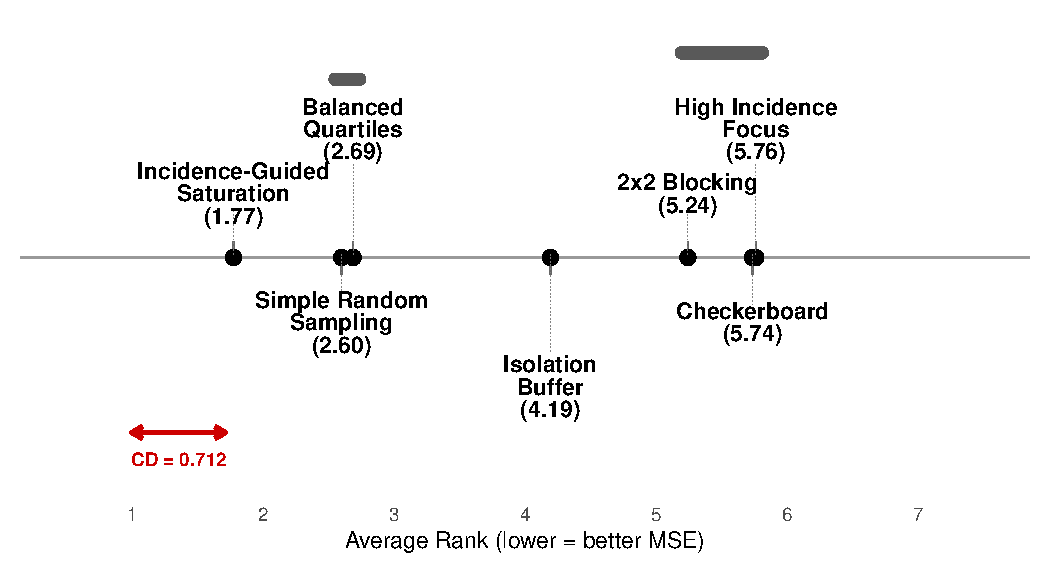
\includegraphics[width=0.72\linewidth]{../figures/app_cd_diagram_rank_queen.pdf}

\caption{Queen contiguity (primary)}
\label{fig:cd-queen}
\end{subfigure}

\vspace{0.5em}
\begin{subfigure}{\linewidth}

\centering
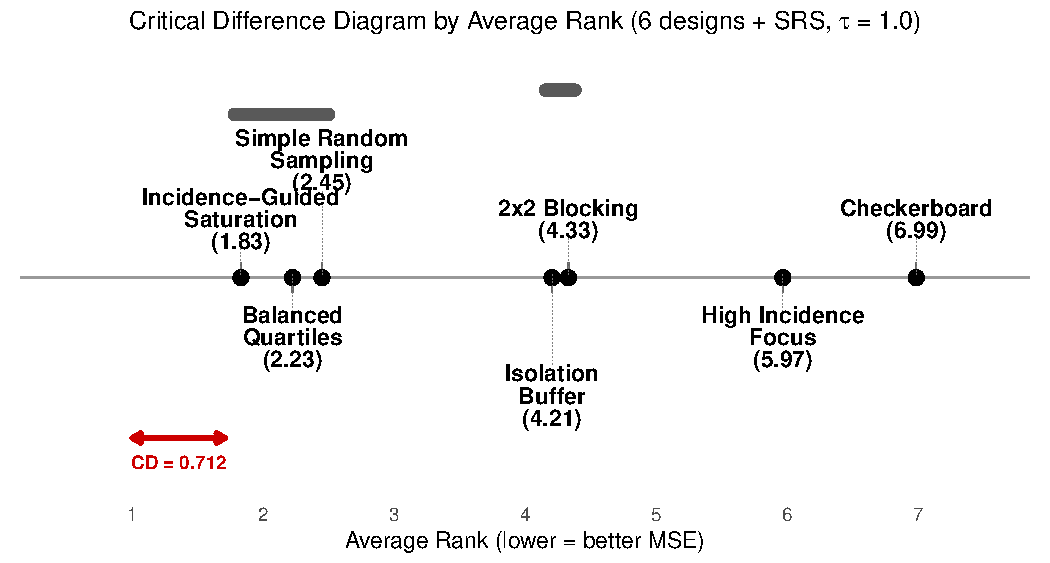
\includegraphics[width=0.72\linewidth]{../figures/app_cd_diagram_rank_rook.pdf}

\caption{Rook contiguity (sensitivity)}
\label{fig:cd-rook}
\end{subfigure}

\caption{Nemenyi critical-difference diagrams for the six designs and simple random sampling (SRS) at $\tau = 1$, pooled over the five incidence configurations. Designs are placed at their average within-block MSE rank, given in parentheses (1 = lowest MSE); gray bars join designs that the Nemenyi comparisons did not separate.}
\label{fig:cd}

\end{figure}

Figure \ref{fig:cd} gives the Nemenyi critical-difference diagrams for
the comparison of the six designs and SRS at \(\tau = 1\), whose results are
reported under Formal statistical comparison (queen contiguity) and Rook
contiguity in the Results. Each design is placed at its average
within-block MSE rank among the six designs and SRS over the 160 blocks of its
neighbor type. The red arrow shows the critical difference, 0.712 at
\(\alpha = 0.05\), and a gray bar joins designs whose pairwise Nemenyi
comparisons were all not significant. Under queen contiguity, the bars join Balanced Quartiles with SRS, and \(2\times2\) Blocking with
Checkerboard and High Incidence Focus. Under rook contiguity, they join
Incidence-Guided Saturation, Balanced Quartiles and SRS, and
Isolation Buffer with \(2\times2\) Blocking. Under
rook contiguity, \(\tau\) is not identified for Checkerboard; its
estimates are kept and flagged.

\begin{figure}[!htb]

\centering
\begin{subfigure}{\linewidth}

\centering
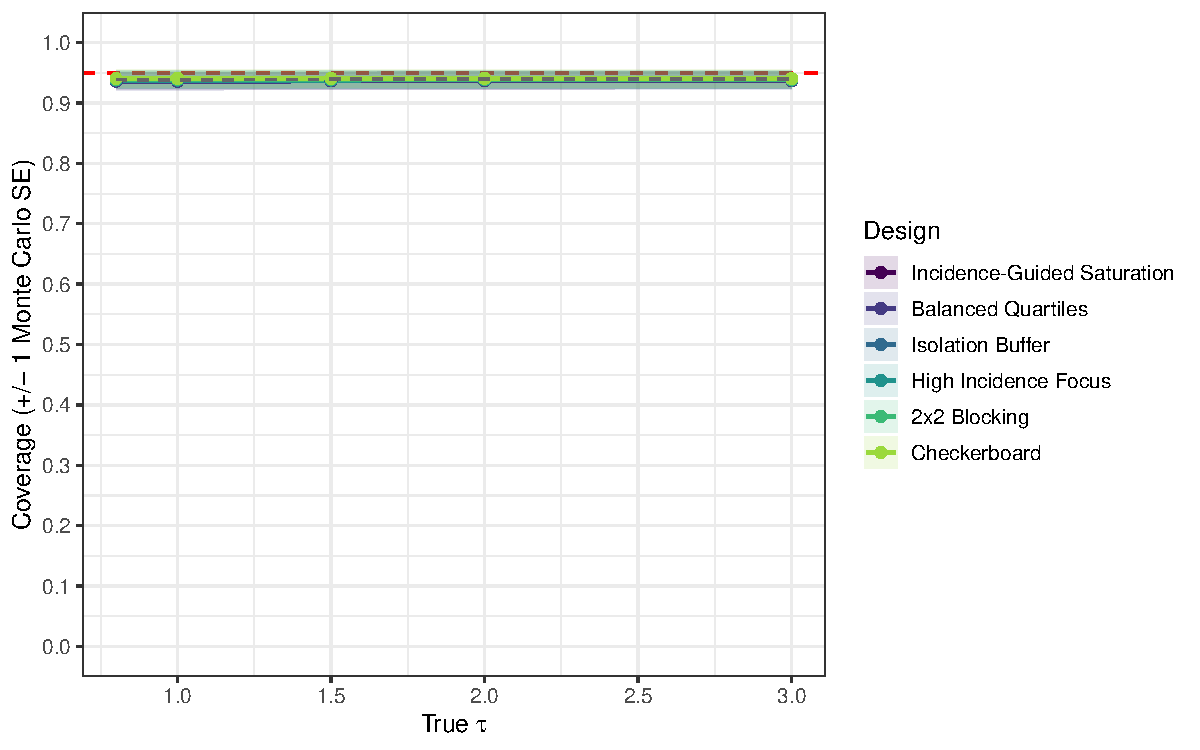
\includegraphics[width=0.5\linewidth]{../figures/app_tau_coverage_queen.pdf}

\caption{Queen contiguity (primary)}
\label{fig:tau-coverage-queen}
\end{subfigure}

\vspace{0.5em}
\begin{subfigure}{\linewidth}

\centering
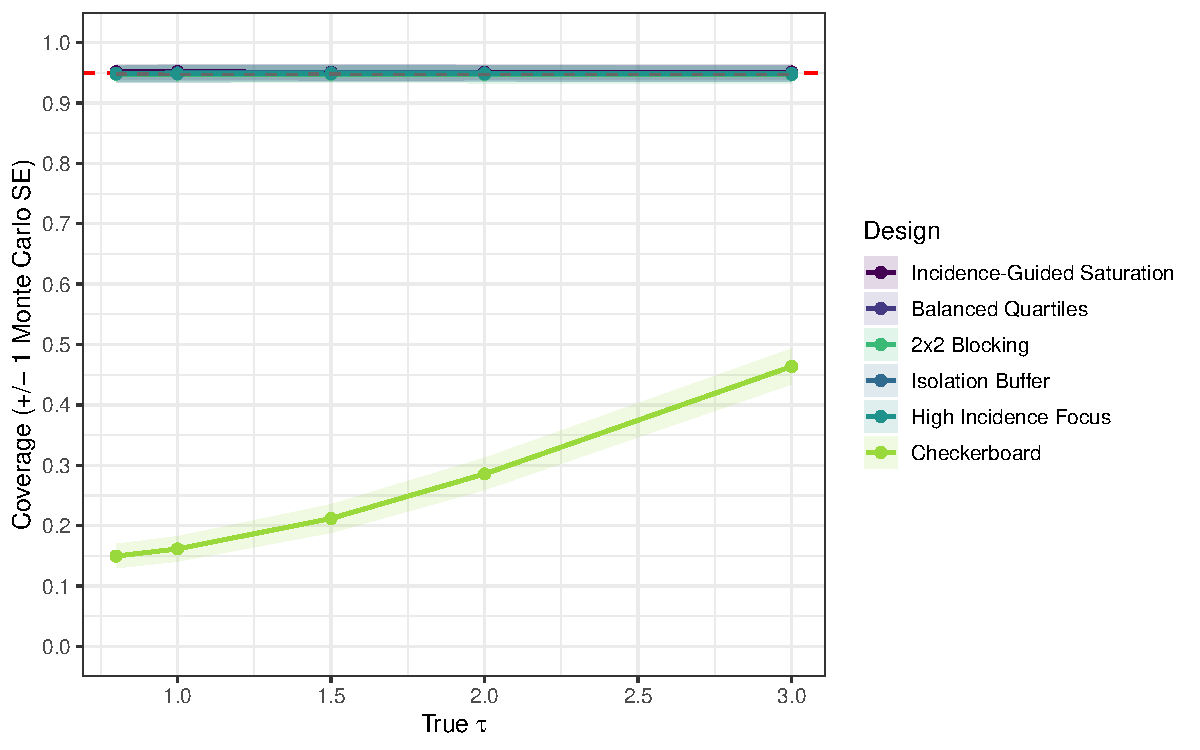
\includegraphics[width=0.5\linewidth]{../figures/app_tau_coverage_rook.pdf}

\caption{Rook contiguity (sensitivity)}
\label{fig:tau-coverage-rook}
\end{subfigure}

\caption{Coverage of the 95\% confidence intervals by design across $\tau \in \{0.8, 1.0, 1.5, 2.0, 3.0\}$, pooled over the five incidence configurations. Each point averages the 160 scenarios of one design at one value of $\tau$. The dashed red line marks the nominal 0.95 level, and the gray dashed line marks the mean coverage of simple random sampling.}
\label{fig:tau-coverage}

\end{figure}

Figure \ref{fig:tau-coverage} gives the coverage of each design across
the five values of \(\tau\), summarized under Stability across treatment
effect sizes. The shaded bands show \(\pm 1\) times the average of the
scenario-level Monte Carlo standard errors of coverage; they describe
the precision of a single scenario's coverage, not of the plotted
average. The legend lists the designs in order of pooled mean MSE at
\(\tau = 1\) for the neighbor type of the panel (Table
\ref{tab:performance}). The vertical axis runs from 0 to 1, so lines
close to 0.95 overlap: all six under queen contiguity, between 0.946 and 0.950, and all but Checkerboard under rook contiguity, between 0.947 and 0.952. The lowest line under rook contiguity, which the legend does not
mark, is Checkerboard, for which \(\tau\) is not identified; its
estimates are kept and flagged. The five values of \(\tau\) share their
assignments and noise.

\section{Rook contiguity figures}\label{s4.-rook-contiguity-figures}

\applabel{S7}{app:rook-figures}This section gives the rook-contiguity
versions of three figures shown for queen contiguity in the detailed grid analysis, as described under Rook
contiguity in the Results. Each has the layout of its queen counterpart,
but designs are ordered for rook contiguity, so the order differs from
that of the queen figure. Under rook contiguity, \(\tau\) is not
identified for Checkerboard (\(WZ = 1 - Z\)); its estimates are kept and
flagged. Figure \ref{fig:mse-rook} corresponds to Figure \ref{fig:mse}.

\begin{figure}[!htb]

\centering
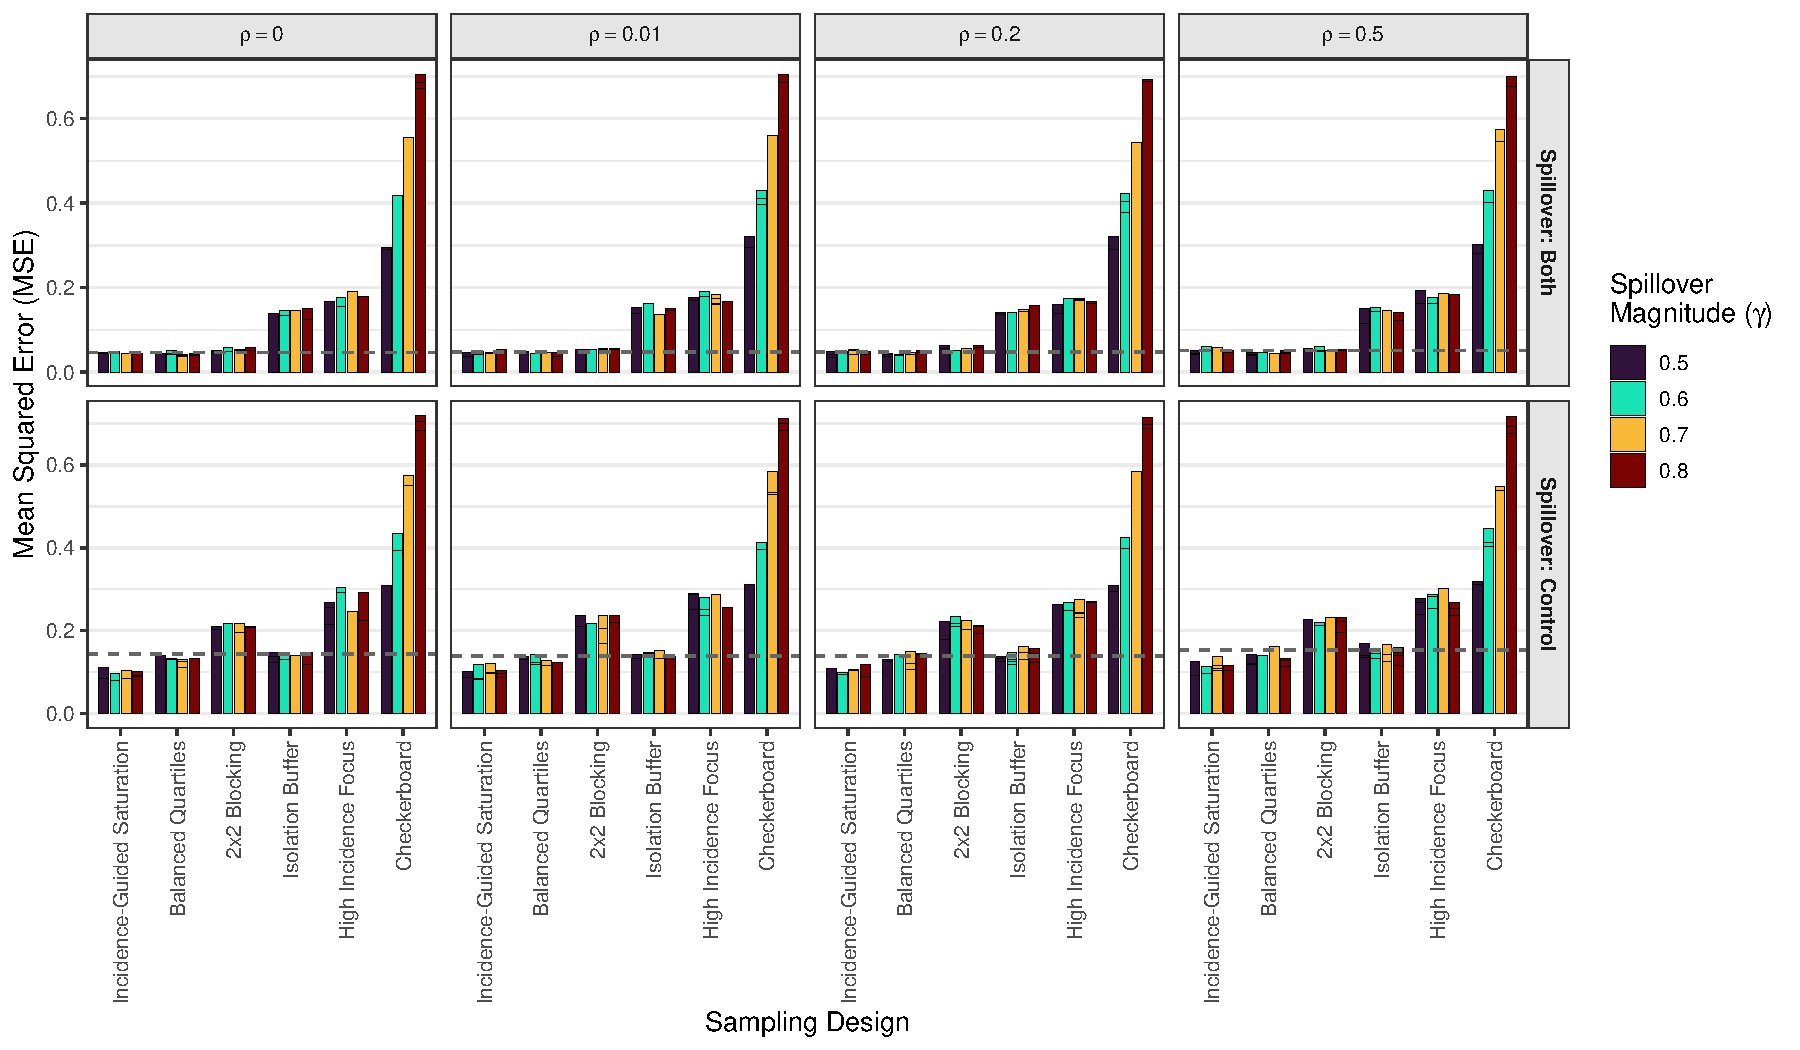
\includegraphics[width=0.75\linewidth]{../figures/fig_mse_by_design_ranked_6design_rook.pdf}

\caption{Mean squared error of the oracle estimate of $\tau$ by design at $\tau = 1$, under rook contiguity; layout as in Figure \ref{fig:mse}. Checkerboard is flagged ($\tau$ not identified).}
\label{fig:mse-rook}

\end{figure}

Figure \ref{fig:coverage-rook} corresponds to Figure \ref{fig:coverage}.
Every design except Checkerboard has coverage close to the nominal
level; Checkerboard's coverage, 0.162 pooled over the five incidence
configurations (Table \ref{tab:performance}), is far below it.

\begin{figure}[!htb]

\centering
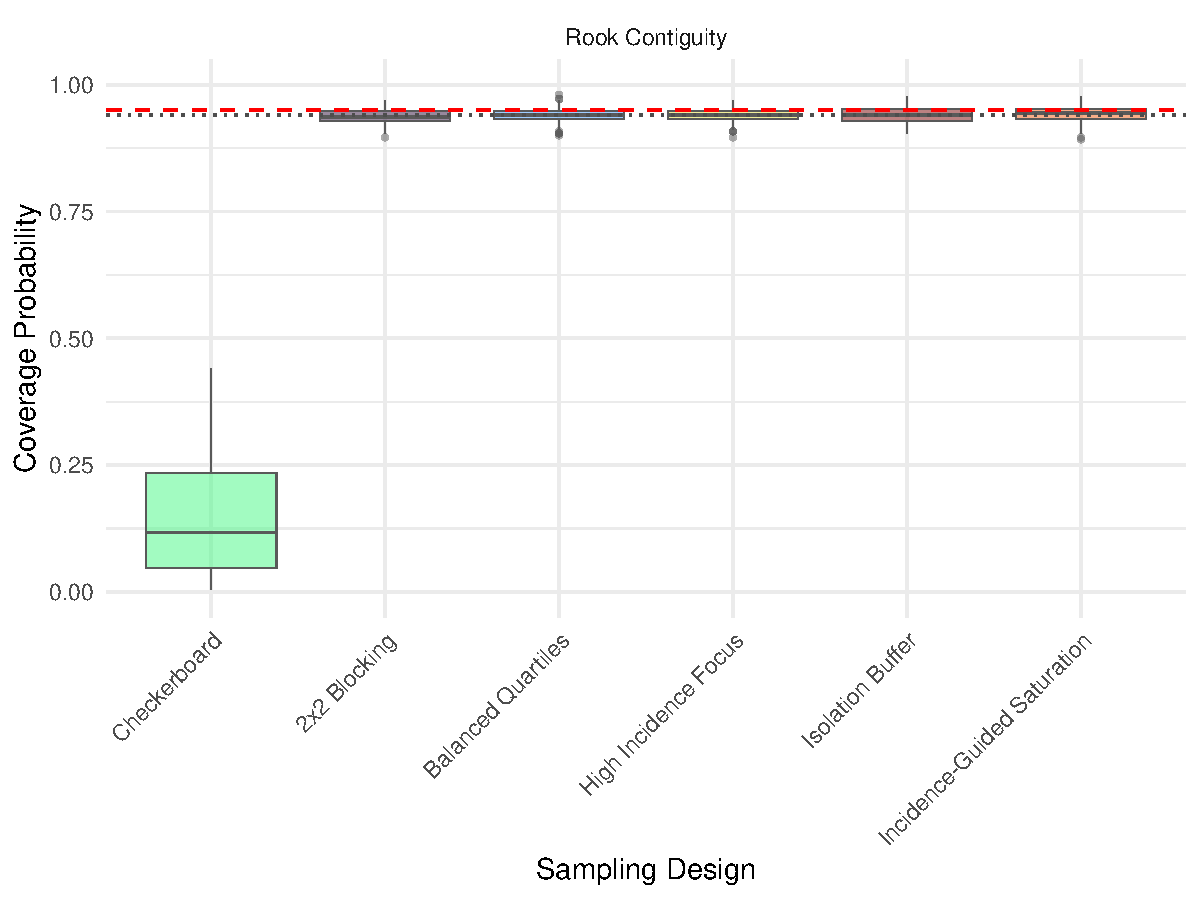
\includegraphics[width=0.55\linewidth]{../figures/fig_coverage_by_design_6design_rook.pdf}

\caption{Coverage of the 95\% confidence intervals by design at $\tau = 1$, under rook contiguity; layout as in Figure \ref{fig:coverage}. Checkerboard is flagged ($\tau$ not identified).}
\label{fig:coverage-rook}

\end{figure}

Figure \ref{fig:biasvar-rook} corresponds to Figure \ref{fig:biasvar}.
Nearly all of Checkerboard's MSE is squared bias, because its
coefficient on \(Z\) estimates \(\tau - \gamma\) (Methods).

\begin{figure}[!htb]

\centering
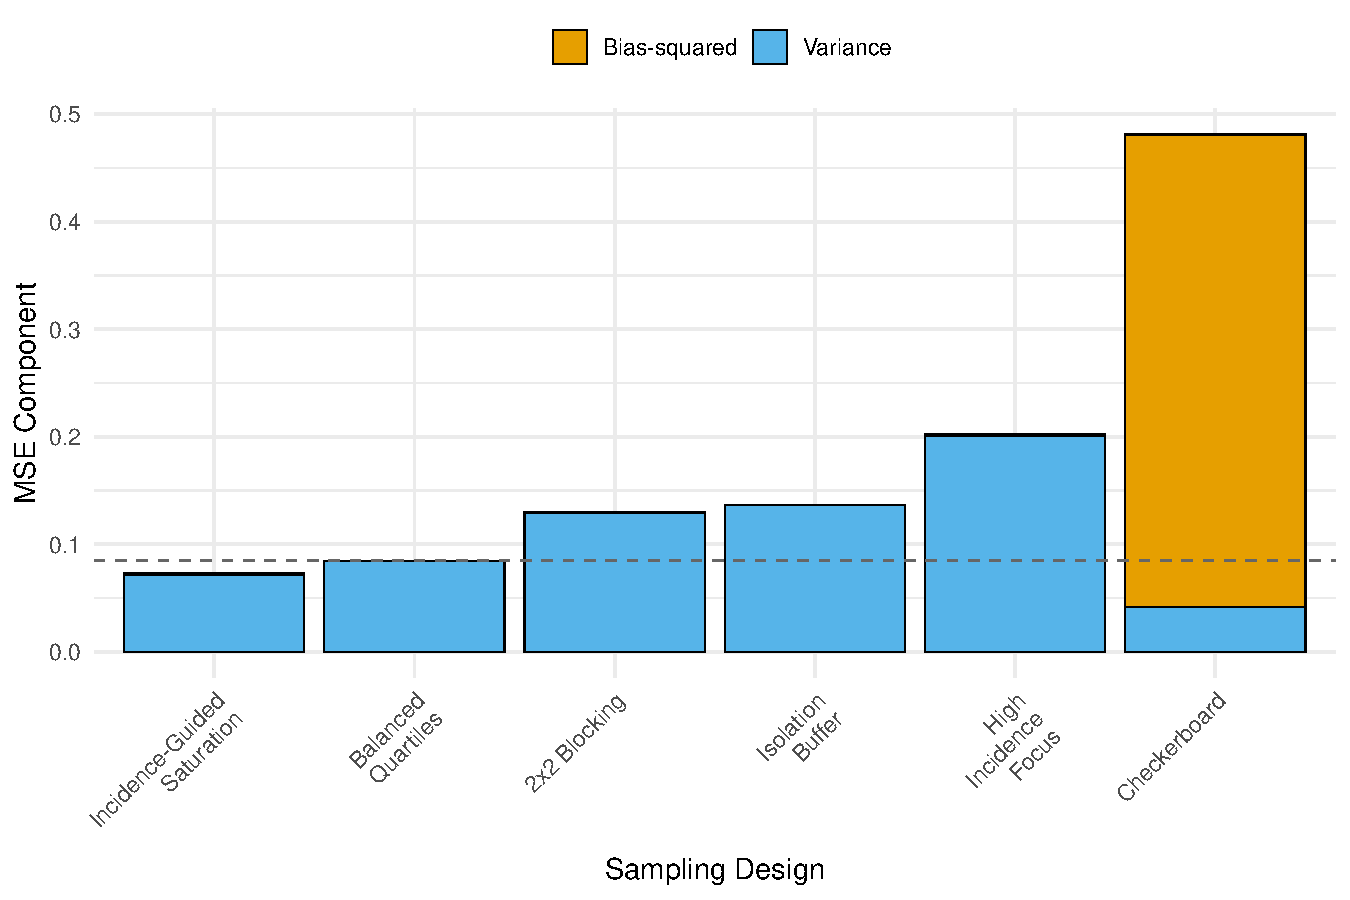
\includegraphics[width=0.55\linewidth]{../figures/fig_biasvar_6design_rook.pdf}

\caption{Squared bias and variance of $\hat\tau$ by design at $\tau = 1$ for the Poisson configuration with $\rho_X = 0.20$, under rook contiguity; layout as in Figure \ref{fig:biasvar}. Checkerboard is flagged ($\tau$ not identified).}
\label{fig:biasvar-rook}

\end{figure}

\FloatBarrier

\section{Oracle and non-oracle
estimates}\label{s5.-oracle-and-non-oracle-estimates}

\applabel{S8}{app:oracle-nonoracle}Table \ref{tab:oracle-nonoracle}
gives the mean squared error, bias, and coverage of the oracle and
non-oracle models for each of the six designs, as summarized under
Non-oracle sensitivity analysis in the Results.

\begin{table}[!htb]

\small
\centering

\caption{Oracle and non-oracle estimates of $\tau$ by design at $\tau = 1$, under queen contiguity (primary) and rook contiguity (sensitivity), pooled over the five incidence configurations. Each entry averages the 160 scenarios of one design and neighbor type. The oracle model has the covariates $Z$, $\text{Spill}$, and $X_k$; the non-oracle model omits $\text{Spill}$. Rows in both panels are in order of oracle MSE under queen contiguity. Under rook contiguity, $\tau$ is not identified for Checkerboard ($WZ = 1 - Z$); its estimates are kept and flagged, and the two models coincide.}
\label{tab:oracle-nonoracle}

\begin{tabular}{>{\raggedright\arraybackslash}p{4.0cm}cccccc}

\toprule
& \multicolumn{3}{c}{Oracle} & \multicolumn{3}{c}{Non-oracle} \\
\cmidrule(lr){2-4}\cmidrule(lr){5-7}
Design & MSE & Bias & Coverage & MSE & Bias & Coverage \\

\midrule
\multicolumn{7}{l}{\textit{Queen contiguity (primary)}} \\
Incidence-Guided Saturation & 0.091 & 0.032 & 0.947 & 0.087 & $-0.123$ & 0.825 \\
Balanced Quartiles & 0.131 & 0.017 & 0.946 & 0.098 & $-0.176$ & 0.786 \\
Isolation Buffer & 0.160 & 0.003 & 0.949 & 0.091 & $-0.175$ & 0.892 \\
High Incidence Focus & 0.245 & 0.031 & 0.948 & 0.219 & $-0.180$ & 0.907 \\
2$\times$2 Blocking & 0.319 & 0.010 & 0.948 & 0.121 & $-0.244$ & 0.727 \\
Checkerboard & 1.087 & 0.001 & 0.950 & 0.108 & $-0.206$ & 0.758 \\

\midrule
\multicolumn{7}{l}{\textit{Rook contiguity (sensitivity)}} \\
Incidence-Guided Saturation & 0.072 & 0.018 & 0.952 & 0.086 & $-0.121$ & 0.825 \\
Balanced Quartiles & 0.084 & 0.008 & 0.948 & 0.097 & $-0.176$ & 0.789 \\
Isolation Buffer & 0.133 & 0.003 & 0.950 & 0.211 & $-0.400$ & 0.536 \\
High Incidence Focus & 0.206 & 0.018 & 0.948 & 0.223 & $-0.192$ & 0.903 \\
2$\times$2 Blocking & 0.128 & 0.004 & 0.948 & 0.128 & $-0.257$ & 0.710 \\
Checkerboard (flagged) & 0.480 & $-0.652$ & 0.162 & 0.480 & $-0.652$ & 0.162 \\

\bottomrule

\end{tabular}

\end{table}

\FloatBarrier

\section{Technical notes}\label{s6.-technical-notes}

\applabel{S9}{app:technical}

\applabel{S9}{app:technical-notes}This section explains two results
reported in the detailed grid analysis: the
growth with \(\tau\) of the bias of Incidence-Guided Saturation, and the rise with \(\tau\) of the coverage of Checkerboard
under rook contiguity. The stored results keep neither \(\hat\rho\) nor
the standard error of each fit, so we re-ran every block for the six
designs, both neighbor types, and all five values of \(\tau\), 2.4
million fits of the oracle model, recording \(\hat\rho\) and the
standard error, and the re-run reproduced the stored results in all
9,600 scenarios. Numbers below that involve \(\hat\rho\), the standard
error, or the terms of Equation \ref{eq:error-decomposition} come from
this re-run; the others come from the stored results.

\subsection{Identification
diagnostics}\label{identification-diagnostics}

Two combinations of design and neighbor type weaken or remove the
information that separates \(\tau\) from the spillover term. Under rook
contiguity, Checkerboard gives \(WZ = 1 - Z\) exactly, because every
neighbor of a treated cluster is a control and every neighbor of a
control is treated. Both spillover covariates then equal
\(\gamma(1 - Z)\), a linear combination of the intercept and \(Z\), so
\(\tau\) is not identified: the fitting routine drops the aliased
spillover column, and the coefficient on \(Z\) estimates
$\tau - \gamma$. The earlier small-grid study noted the same
consequence of exact collinearity between treatment and spillover
exposure, \(\hat\beta \approx \beta - \psi\) in its notation. The
non-oracle model has no spillover column to drop, but its Checkerboard
estimates under rook contiguity have the same defect. Under queen
contiguity, each of the 64 interior clusters has four treated and four
control neighbors, so \(WZ = 1/2\) at every interior cluster. Under the
control-only regime the spillover covariate then equals
\((\gamma/2)(1 - Z)\) at those clusters, a linear combination of the
intercept and \(Z\), and only the 36 clusters on the grid boundary carry
information that separates it from the intercept and \(Z\); \(\tau\) is
identified, but imprecisely. Under the both-arms regime it is the
constant \(\gamma/2\) at interior clusters, confounded with the
intercept but not with \(Z\). Isolation Buffer under rook contiguity can
also, rarely, draw exactly the checkerboard pattern, a maximal
independent set that equals one color class of the grid. This happened
in 4 of its 40,000 rook draws and affected one fit in each of 20
scenarios, 4 at each value of \(\tau\). We flag every fit in which the
fitting routine reports an aliased column and every scenario in which
some draw has \(\text{rank}([1, Z, WZ]) < 3\). Aliased estimates are
kept in all summaries. In the exhibits, we flag Checkerboard under rook
contiguity, where every fit is aliased; the Isolation Buffer scenarios,
each with one aliased fit among its 250, are noted here and carry no
flag in the exhibits.

\subsection{\texorpdfstring{Estimation error and its dependence on
\(\tau\)}{Estimation error and its dependence on \textbackslash tau}}\label{estimation-error-and-its-dependence-on-tau}

For one fit \((k, j)\), write \(Y\), \(Z\), and \(\epsilon\) for
\(Y_{kj}\), \(Z_{kj}\), and \(\epsilon_{kj}\) (Simulation design,
resampling, and metrics). Let \(V = [1, Z, S(Z), X_k]\) be the
\(100 \times 4\) covariate matrix of the oracle model, so that Equation
\ref{eq:outcome} reads \((I - \rho W)Y = V\theta + \epsilon\) with
\(\theta = (0, \tau, 1, \beta)^\top\). Let \(A = (I - \rho W)^{-1}\) and
\(V^{+} = (V^\top V)^{-1}V^\top\), and for a vector \(v\) write
\([V^{+}v]_Z\) for the coefficient on \(Z\) when \(v\) is regressed on
the columns of \(V\) by least squares. Given \(\hat\rho\), the estimated
coefficients are \(V^{+}(I - \hat\rho W)Y\) (Estimation). Because
\((I - \hat\rho W)Y = V\theta + \epsilon + (\rho - \hat\rho)WY\) and
\(WY = WA(V\theta + \epsilon)\), \begin{equation}
\hat\tau - \tau = [V^{+}\epsilon]_Z + (\rho - \hat\rho)\,h + \tau(\rho - \hat\rho)\,g,
\label{eq:error-decomposition}
\end{equation} where \[
g = [V^{+}WAZ]_Z, \qquad h = [V^{+}WA\{S(Z) + \beta X_k + \epsilon\}]_Z.
\] The first term has mean zero given \(Z\) and \(X_k\). The last term
carries a factor of \(\tau\). It is present exactly when \(g \neq 0\),
where \(g\) is the coefficient on \(Z\) when the lagged treatment
\(WAZ = WZ + \rho W^2 Z + \rho^2 W^3 Z + \cdots\) is regressed on the
model's own covariates, and its sign and size are set by the error in
\(\hat\rho\). The concentrated likelihood depends on \(Y\) only through
the residual sum of squares of \((I - \tilde\rho W)Y\) on \(V\), and the
part of that residual that involves \(\tau\) is
\(\tau(\rho - \tilde\rho)\) times the residual of \(WAZ\) on \(V\). If
\(WAZ\) lies in the column space of \(V\), that part vanishes for every
\(\tilde\rho\), so \(\hat\rho\) is the same at every value of \(\tau\);
if in addition \(g = 0\), then \(\hat\tau - \tau\) is the same at every
value of \(\tau\). Equation \ref{eq:error-decomposition} held on every
re-run fit, with a largest residual of \(4.2\times10^{-13}\); for
Checkerboard under rook contiguity it held in the reduced form given
below.

Two consequences of Equation \ref{eq:error-decomposition} explain the
results for \(\tau\) reported in the detailed grid analysis.

First, for designs whose treated clusters have treated neighbors, the
last term gives a small positive bias that grows with \(\tau\). Under
queen contiguity, pooled over the 160 blocks, the bias of
Incidence-Guided Saturation rose from 0.029 at \(\tau = 0.8\)
to 0.047 at \(\tau = 3\) (Stability across treatment effect sizes),
while that of Isolation Buffer stayed between 0.002 and 0.004. Almost
all of the rise is the last term of Equation
\ref{eq:error-decomposition}. In our fits, \(\hat\rho\) was biased
downward by about 0.06 on average (for Incidence-Guided Saturation, by 0.071 at \(\tau = 0.8\) and 0.054 at \(\tau = 3\)). We
observed this downward bias in these simulations; we did not derive it
or check it against a published finite-sample result. With
\(\rho - \hat\rho\) positive on average, the last term is positive and
grows with \(\tau\) for any design with \(g > 0\). For Incidence-Guided
Saturation, \(g\) averaged 0.371 over the queen fits, and the
last term contributed 0.021 of the bias at \(\tau = 0.8\) and 0.043 at
\(\tau = 3\); the first term contributed 0.001 at both values, and the
second 0.007 and 0.002. For Isolation Buffer, \(g\) averaged 0.020, and
the last term contributed 0.001 and 0.004. Most of the difference in
\(g\) comes from the control-only regime. Under the both-arms regime
with \(\rho = 0\), the lagged treatment is \(WZ = S(Z)/\gamma\), one of
the covariates, so \(g = 0\) for every design. Under the control-only
regime, \(WZ = S(Z)/\gamma + Z \circ WZ\), and at \(\rho = 0\), \(g\) is
close to the average share of treated neighbors among treated clusters.
That share is 0.57 for Incidence-Guided Saturation, whose
treated clusters are concentrated in the high-saturation quadrants, and
exactly 0 for Isolation Buffer, whose treated clusters have no treated
neighbors. For Isolation Buffer, \(Z \circ WZ = 0\), so the two regimes
define the same spillover covariate and the same \(g\), which is 0 at
\(\rho = 0\) and about 0.06 at \(\rho = 0.5\); at \(\rho = 0\), its
\(\hat\rho\) and its estimation error were the same at every value of
\(\tau\), up to the optimizer's tolerance.

The same term explains why the control-only MSE of Incidence-Guided
Saturation rose from 0.131 at \(\tau = 0.8\) to 0.182 at
\(\tau = 3\) while that of Isolation Buffer did not. Under that regime,
averaged over the 80 queen blocks, the variance of the last term of
Equation \ref{eq:error-decomposition} rose from 0.008 to 0.061 for
Incidence-Guided Saturation, while the variance of the rest of
the error changed little (0.119 and 0.115). The variance of the last
term grew more slowly than \(\tau^2\) because \(\hat\rho\) became less
variable as \(\tau\) grew. For Isolation Buffer, the variance of the
last term stayed below 0.0002. The rise in bias slowed at larger values
of \(\tau\) for a related reason: the part of the likelihood that
involves \(\tau\) sharpens it around the true \(\rho\) as \(\tau\)
grows, so the downward bias of \(\hat\rho\) shrank.

Second, the decomposition explains why the coverage of Checkerboard
under rook contiguity rose with \(\tau\). Under rook contiguity,
Checkerboard's coverage rose from 0.150 at \(\tau = 0.8\) to 0.464 at
\(\tau = 3\) (Stability across treatment effect sizes), although its
coefficient on \(Z\) estimates \(\tau - \gamma\) at every value of
\(\tau\). For this design \(WZ = 1 - Z\), and because \(W\) is
row-standardized, \(W^2 Z = W(1 - Z) = Z\). The powers of \(W\) applied
to \(Z\) therefore alternate between \(1 - Z\) and \(Z\), and
\(WAZ = \{(1 - Z) + \rho Z\}/(1 - \rho^2)\) lies in the span of the
intercept and \(Z\). The derivation of Equation
\ref{eq:error-decomposition} applies with the aliased spillover column
dropped, \(V = [1, Z, X_k]\) and
\(\theta = (\gamma, \tau - \gamma, \beta)^\top\), so that
\(\tau - \gamma\) takes the place of \(\tau\), and
\(g = -1/(1 + \rho)\). Two consequences follow: \(\hat\rho\) is the same
at every value of \(\tau\), and \[
\hat\tau - \tau = -\gamma + \delta + (\tau - \gamma)\,\frac{\hat\rho - \rho}{1 + \rho},
\] where \(\delta\) collects the first two terms of that decomposition
and, like \(\hat\rho\), does not depend on \(\tau\). The error in
\(\hat\rho\) is therefore multiplied by \(\tau - \gamma\), which grows
with \(\tau\). The mean standard deviation of \(\hat\tau\) rose from
0.202 at \(\tau = 0.8\) to 0.327 at \(\tau = 3\), and the standard error
tracked it, rising on average from 0.199 to 0.322. With the bias held
near \(-\gamma\), wider intervals covered \(\tau\) more often. The rise
was largest at \(\rho = 0\) (coverage 0.157 to 0.562) and smallest at \(\rho = 0.5\) (0.142 to 0.284), consistent with the factor
\(1/(1 + \rho)\). The same term raised the MSE from 0.477 to 0.567.
About three quarters of that increase was variance,
\((n-1)\text{SD}^2/n\) averaged over scenarios (Section
\ref{app:mechanics}), which rose from 0.041 to 0.109. The other quarter
was squared bias, which rose from 0.436 to 0.458 because \(\hat\rho\)
was biased slightly downward, moving the mean bias from \(-0.650\) to
\(-0.667\). The higher coverage at large \(\tau\) reflects wider
intervals around the wrong quantity, not a recovery of \(\tau\).

\FloatBarrier

\section{Observed-incidence application
detail}\label{s7.-observed-incidence-application-detail}

\applabel{S10}{app:nc}The primary application numbers come from the aggregate performance and allocation-risk summaries of the main run and of the separate tail refinement. Annual tables average the six queen parameter pairs equally, without pooled Monte Carlo intervals. Each random draw used a fixed, reproducible seed. An independent check recomputed performance from the stored fits, checked annual treatment budgets and regional orderings, and checked the allocations and outcomes reused from the main run in the tail refinement. The county death-certificate source data are restricted and not publicly available; only 58-cluster summaries are reported.

For randomized designs, the prespecified refinement schedule allowed $J=100,200,400$ and $R=100,200,400,1000,2000,4000$; whichever source of Monte Carlo error, allocations or outcomes, contributed more to the shortfall from the precision targets was extended. All randomized designs met the targets at $J=100$ and $R=100$. For designs with a single possible assignment, only outcomes were extended. If
an allocation occurs \(n_a\) times among \(J\) draws, its risk estimate
enters the mean with weight \(n_a/J\). The variance due to outcome noise therefore involves squared weights \((n_a/J)^2\), not \(n_a/J^2\) as if
duplicate estimates were independent. Bias and coverage use the same accounting of frequencies and covariances. The overall precision includes both variation across assignments and outcome noise given an assignment; a design whose sampled assignments happened to coincide is distinguished from one with only one possible assignment. Approximate Monte Carlo standard errors of setting-specific differences between designs treat the designs' random draws as independent, whereas averages across settings or models do not assume that shared allocations are independent.

Estimated risk variance is reported raw and with its outcome Monte Carlo
noise contribution subtracted. Signed corrected estimates are retained
rather than silently truncated; none is negative in the NC refinement.
Quantiles and worst-decile means use noisy estimated conditional risks.
To avoid selection bias, worst-decile assignments were identified with one half of the simulated outcomes and evaluated with the other half, and the roles of the two halves were then reversed. The Jaccard overlap of the two worst deciles describes sampled tail membership, not a confidence interval or population tail probability. For a design with only one possible assignment, an overlap of one is uninformative.

The fixed regional criterion is \(C=3s_P+1.5s_K+1.5s_D+c/d_{\max}\), where \(s_P\), \(s_K\) and \(s_D\) are the standard deviations of regional population, cluster and county shares. Here \(c\) averages within-region distances to regional centers and \(d_{\max}\) is the maximum pairwise distance between the projected cluster coordinates. Candidates use standardized projected coordinates and are selected
without outcome performance. The fixed groups used by $2\times2$ Blocking contain one to eight clusters, with one single-cluster group per year; yearly total treatments are 28, 31, 27 and 29.
Table \ref{tab:nc-order} documents alternative summaries before
performance evaluation.

\begin{table}[!htb]
\small
\centering

\caption{Regional ordering from highest to lowest summary, using the fixed region IDs in Figure \ref{fig:nc-regions}. Primary mean ranks weight clusters equally; pooled regional rates weight cluster rates by population.}
\label{tab:nc-order}

\begin{tabular}{lrrr}
\toprule
Year & Mean cluster rank & Mean cluster rate & Pooled regional rate \\
\midrule
2018 & 2,1,3,4 & 2,4,1,3 & 4,3,2,1 \\
2019 & 4,2,3,1 & 4,2,3,1 & 4,3,1,2 \\
2020 & 2,4,1,3 & 2,4,1,3 & 4,3,2,1 \\
2021 & 2,1,4,3 & 2,4,1,3 & 4,3,1,2 \\

\bottomrule
\end{tabular}
\end{table}
\begin{figure}[!htb]
\centering
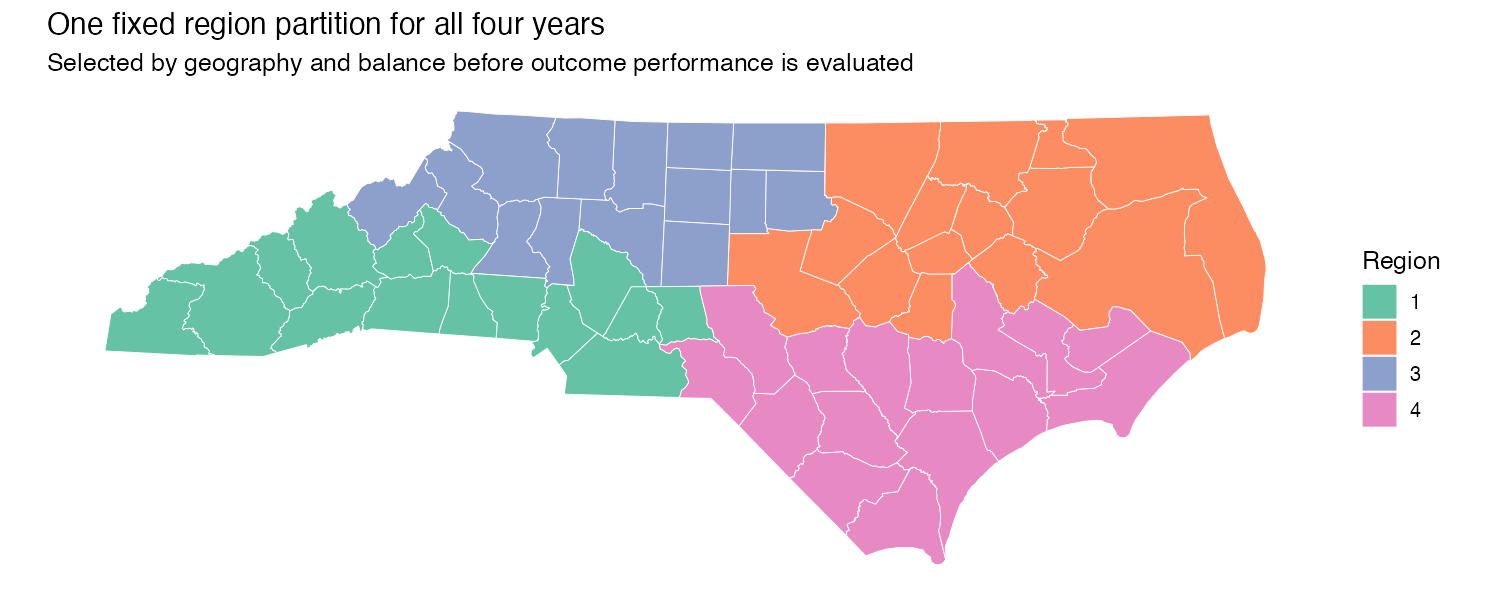
\includegraphics[width=0.85\linewidth]{../figures/real_sud/regions.png}

\caption{Fixed four-region partition used by both saturation strategies in all years, chosen from 250 geographic candidates before outcome evaluation.}
\label{fig:nc-regions}

\end{figure}
\begin{figure}[!htb]
\centering
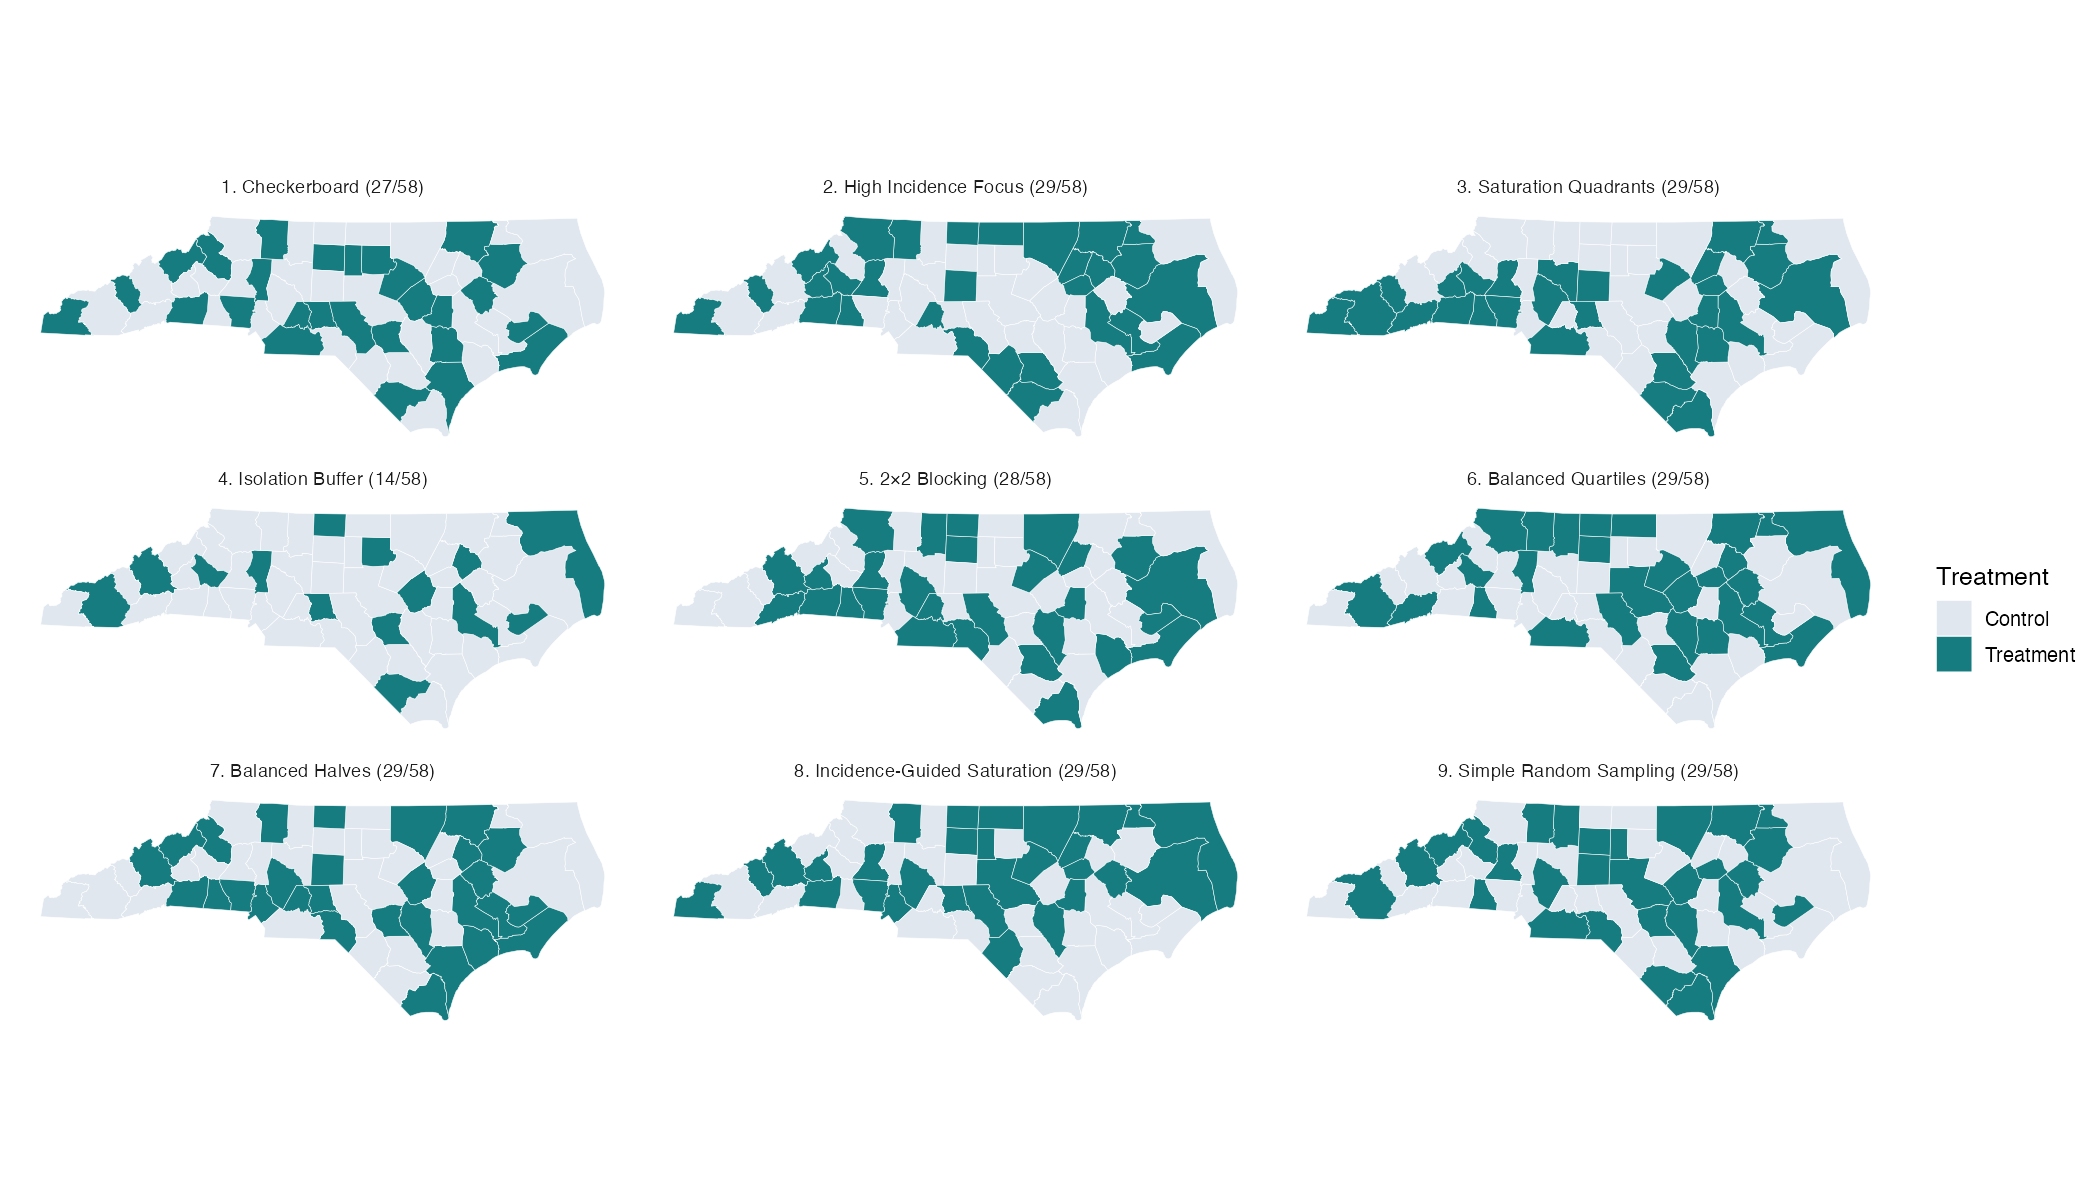
\includegraphics[width=\linewidth]{../figures/real_sud/design_examples.png}

\caption{One illustrative queen assignment from each application strategy using 2018 observed incidence and fixed geography. These sampled assignments illustrate the adaptations; they were not selected by observed performance.}
\label{fig:nc-examples}

\end{figure}
\begin{figure}[!htb]
\centering
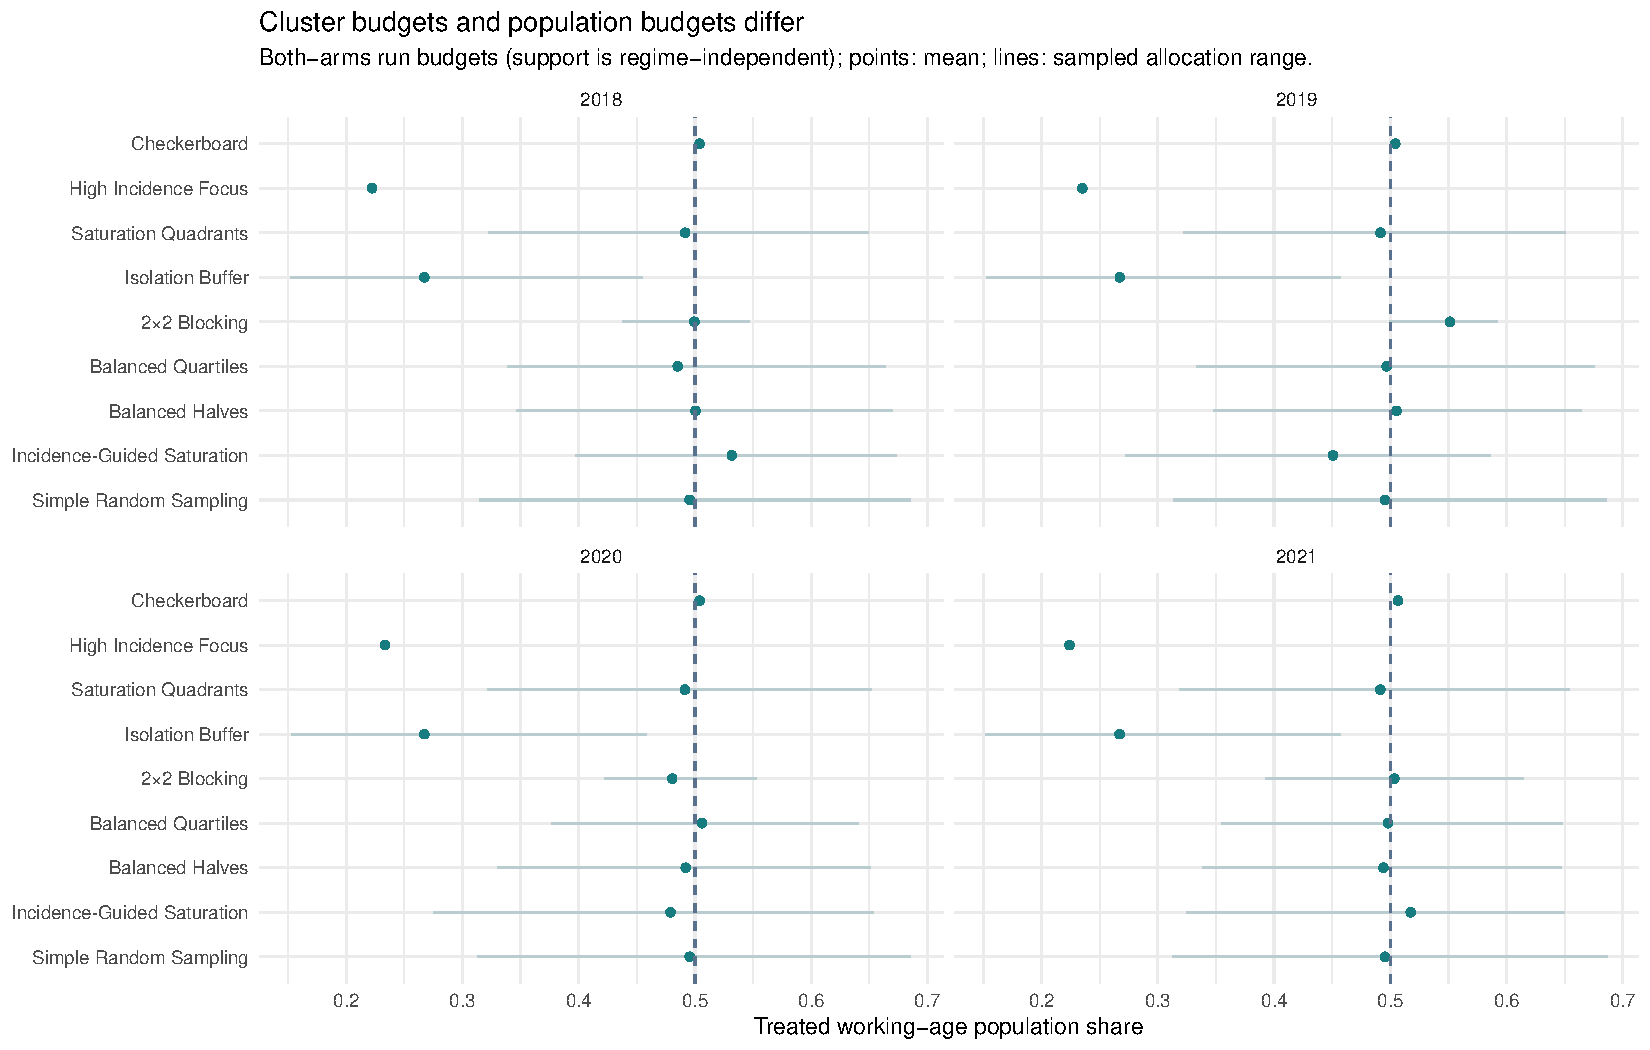
\includegraphics[width=\linewidth]{../figures/real_sud/population_shares.pdf}

\caption{Annual population shares treated under primary queen assignments, using the both-arms runs (the set of possible assignments does not depend on the regime). Points mark the mean and lines the range over sampled allocations. Designs whose assignments do not depend on annual incidence share performance across years, but their annual population shares are recalculated. Population aged 18--64 is geographic reach rather than education-participant enrollment.}
\label{fig:nc-pop}

\end{figure}
\begin{figure}[!htb]
\centering
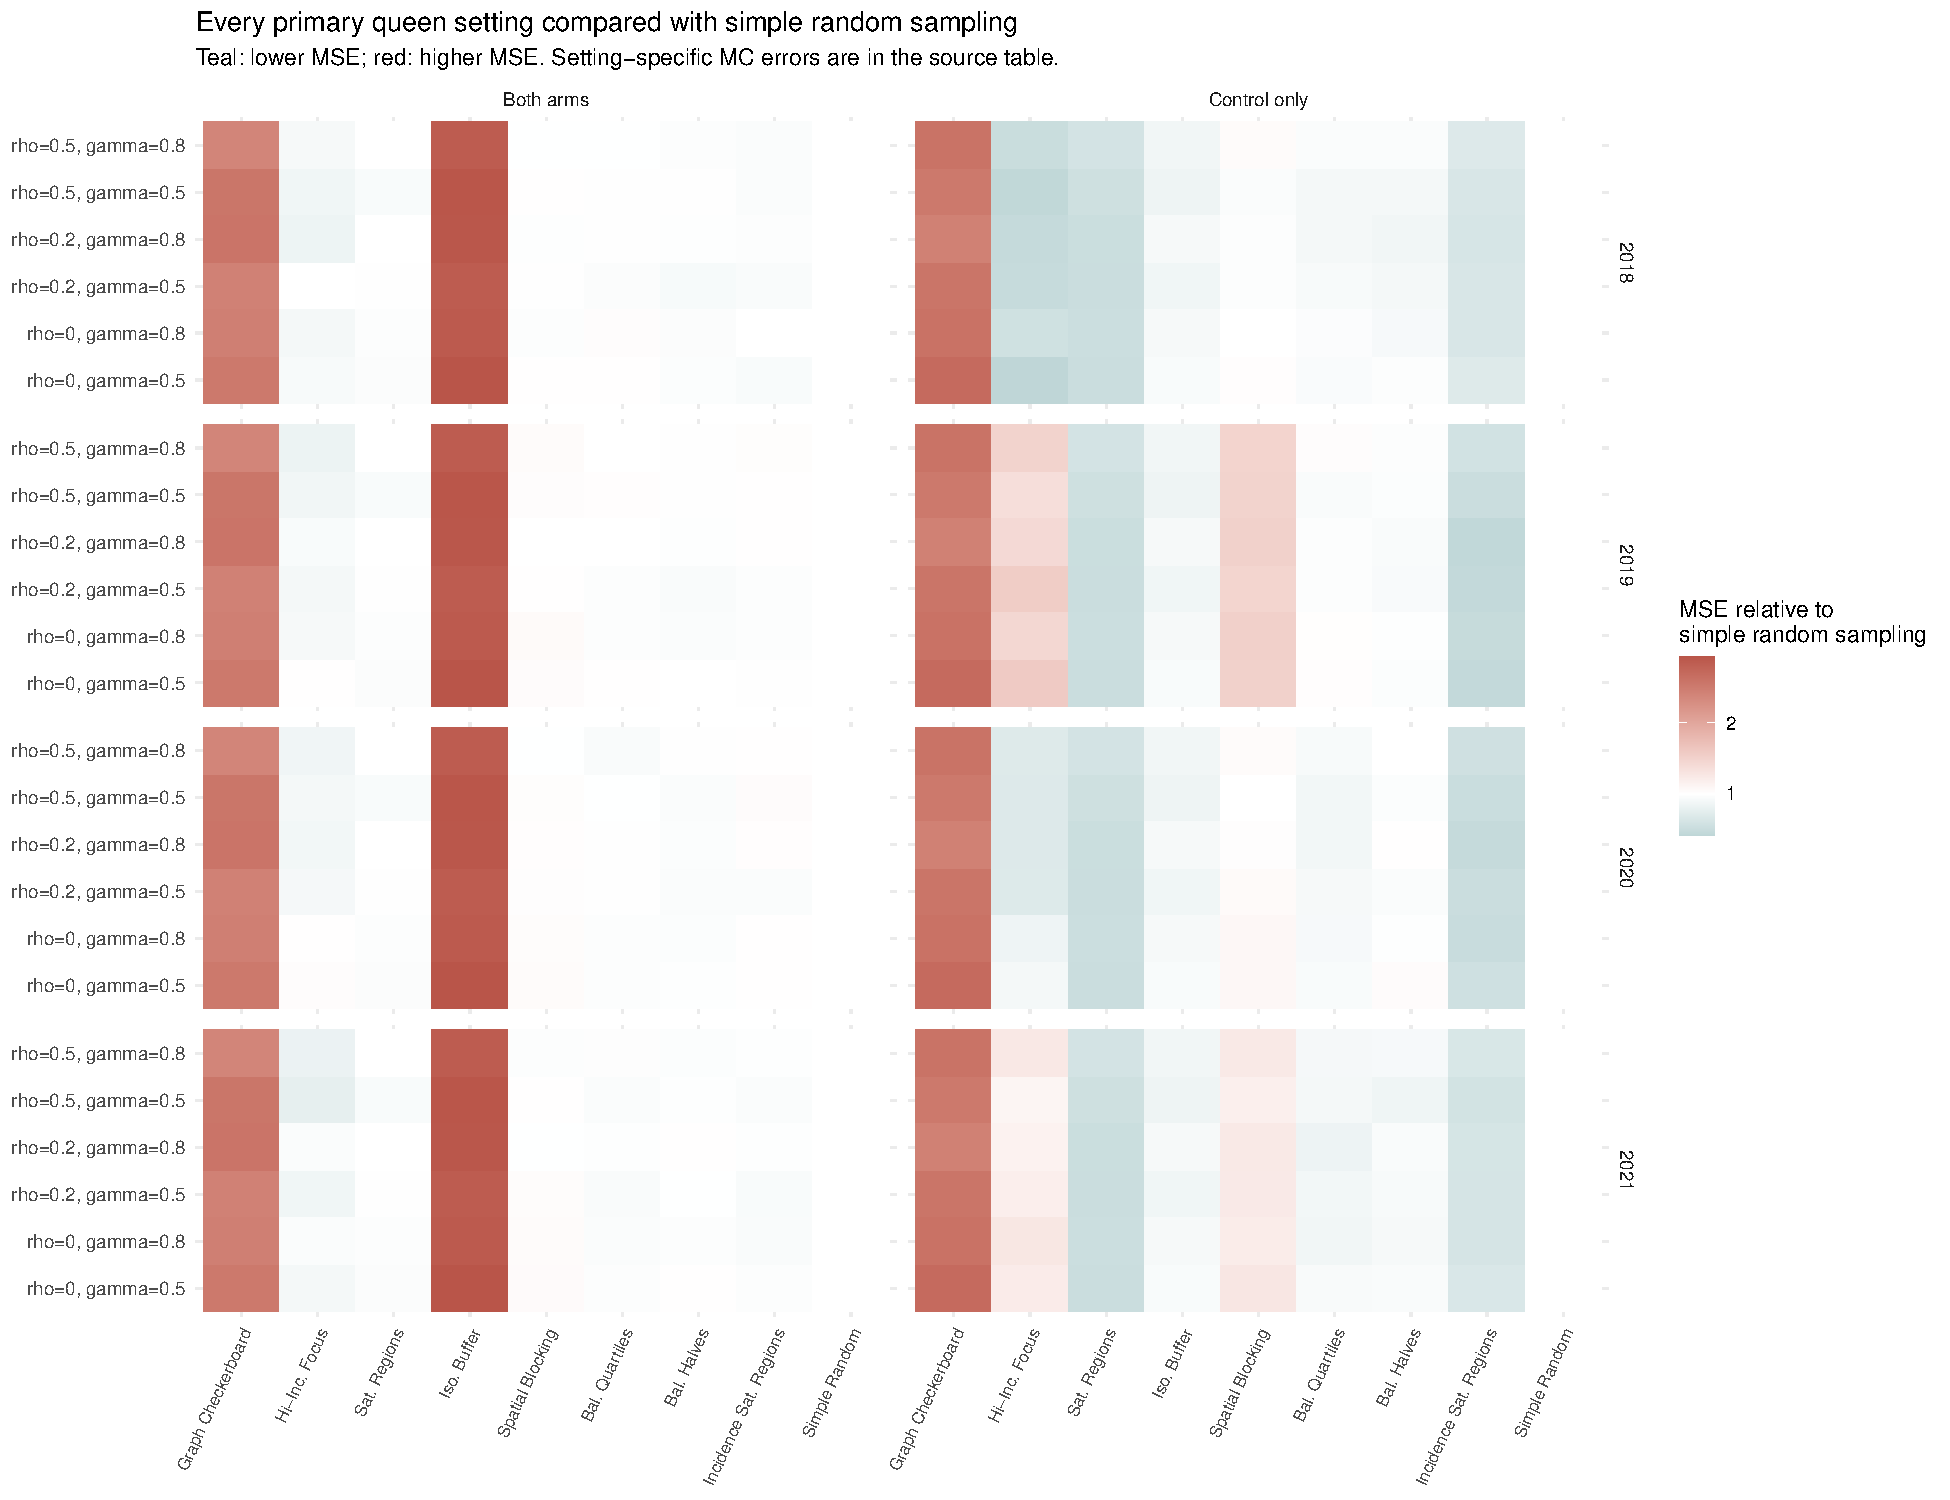
\includegraphics[width=\linewidth]{../figures/real_sud/primary_setting_ratios.pdf}

\caption{Primary queen setting-specific mean MSE ratios to year-matched SRS. Teal cells have lower MSE than SRS and red cells higher; setting-specific Monte Carlo errors are in the source table. Parameters and spillover regimes are kept separate; this plot does not pool neighbor definitions.}
\label{fig:nc-setting-ratios}

\end{figure}

Table \ref{tab:nc-annual} retains MSE, bias and coverage for every design in every year; budgets are in Table \ref{tab:nc-budgets}. More granular setting-specific results,
precision components, residual treatment information and warning and failure records are kept as aggregate output tables. The absence of warnings and failures is a verified result, not a sign that diagnostics were skipped.

\begin{figure}[!htb]

\centering
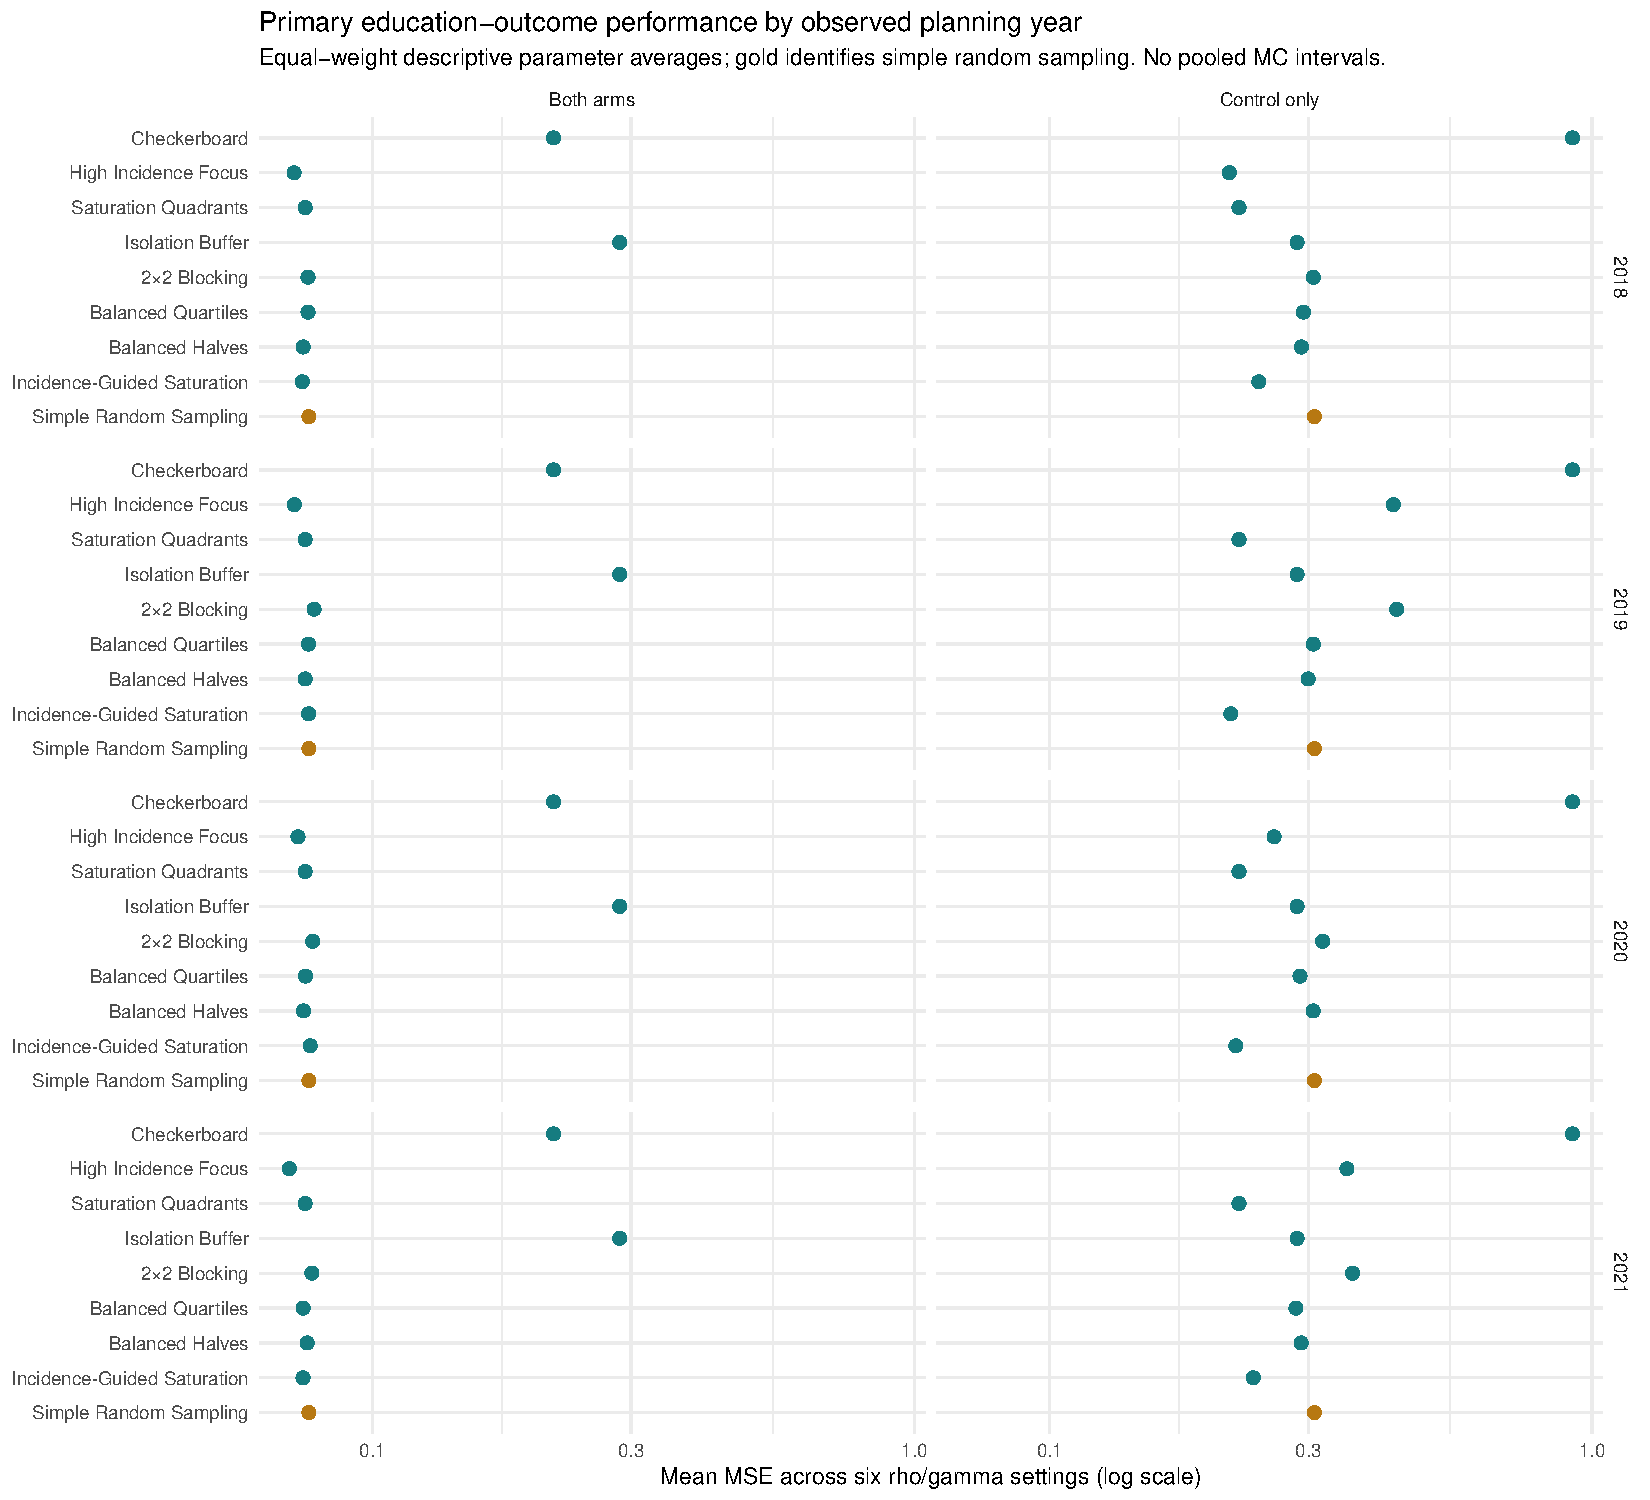
\includegraphics[width=\linewidth]{../figures/real_sud/primary_yearly_mse.pdf}

\caption{Completed primary application: mean MSE by design, planning year and spillover regime, queen contiguity and education outcome. Each entry equally averages the six $\rho/\gamma$ pairs, and simple random sampling is shown in gold. Both regime columns use a common logarithmic MSE scale. Years that share the same simulations are repeated reporting, not independent replications; pooled Monte Carlo intervals are not supplied.}
\label{fig:nc-mse-detail}

\end{figure}
\begin{figure}[!htb]

\centering
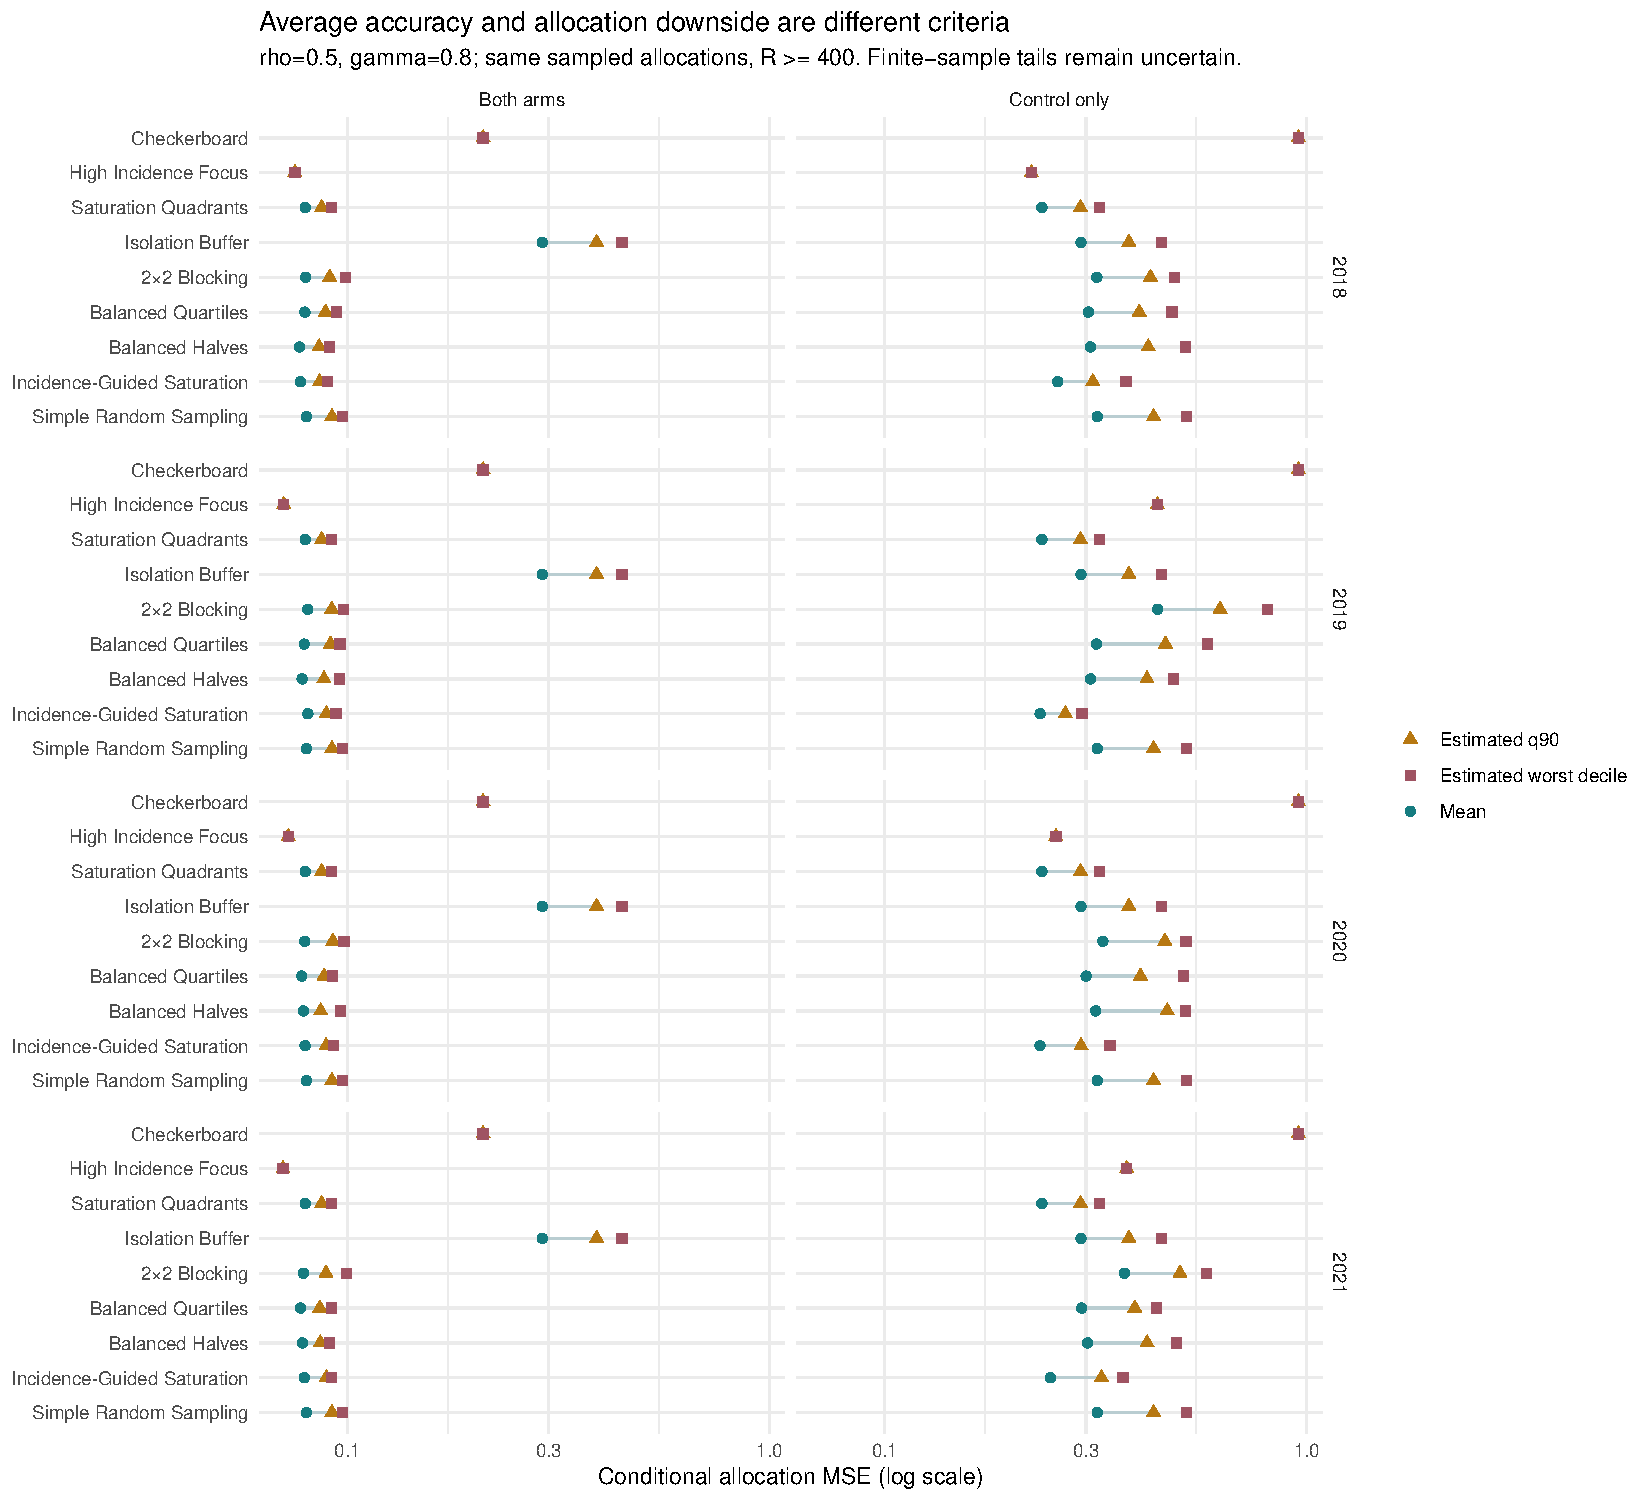
\includegraphics[width=\linewidth]{../figures/real_sud/refined_allocation_risk.pdf}

\caption{Allocation-specific conditional MSE in the refined primary queen setting $\rho=0.5,\gamma=0.8$, by year and spillover regime. Mean MSE, the estimated 90th percentile of allocation-specific MSE and the estimated worst-decile mean summarize the same $J=100$ sampled assignments, with at least 400 independent outcomes per assignment of a randomized design or 1,000 for designs with a single possible assignment. These tail estimates, based on a finite number of outcomes, are descriptive, with uncertain membership; they are not quantiles of realized errors or a fresh allocation confirmation.}
\label{fig:nc-risk}

\end{figure}

\begin{table}[!htb]
\footnotesize
\centering

\caption{Primary queen application performance by design and planning year. Each entry averages the six $\rho/\gamma$ pairs of one spillover regime with equal weight; MSE, bias and coverage of the corrected $t$ interval are Monte Carlo estimates. Checkerboard, Saturation Quadrants, Isolation Buffer and SRS use the same simulations in every year, because annual incidence enters neither their allocation nor the outcome model, so their rows repeat; repeated values are not independent annual confirmation. Treatment counts and population shares are in Table \ref{tab:nc-budgets}.}
\label{tab:nc-annual}
% SOURCE: application/results/real_sud_rev_20261002/exhibits/yearly_primary_design_means.csv

\begin{tabular}{llrrrrrr}
\toprule
& & \multicolumn{3}{c}{Both arms} & \multicolumn{3}{c}{Control only} \\
\cmidrule(lr){3-5}\cmidrule(lr){6-8}
Design & Year & MSE & Bias & Coverage & MSE & Bias & Coverage \\
\midrule
Checkerboard & 2018 & 0.21591 & -0.0074 & 0.949 & 0.92036 & 0.0100 & 0.948 \\
 & 2019 & 0.21591 & -0.0074 & 0.949 & 0.92036 & 0.0100 & 0.948 \\
 & 2020 & 0.21591 & -0.0074 & 0.949 & 0.92036 & 0.0100 & 0.948 \\
 & 2021 & 0.21591 & -0.0074 & 0.949 & 0.92036 & 0.0100 & 0.948 \\
\addlinespace
High Incidence Focus & 2018 & 0.07172 & 0.0160 & 0.948 & 0.21426 & 0.0237 & 0.948 \\
 & 2019 & 0.07180 & 0.0063 & 0.951 & 0.43019 & 0.0227 & 0.945 \\
 & 2020 & 0.07292 & 0.0094 & 0.946 & 0.25918 & 0.0327 & 0.946 \\
 & 2021 & 0.07031 & 0.0104 & 0.951 & 0.35318 & 0.0296 & 0.945 \\
\addlinespace
Saturation Quadrants & 2018 & 0.07518 & 0.0208 & 0.949 & 0.22329 & 0.0464 & 0.941 \\
 & 2019 & 0.07518 & 0.0208 & 0.949 & 0.22329 & 0.0464 & 0.941 \\
 & 2020 & 0.07518 & 0.0208 & 0.949 & 0.22329 & 0.0464 & 0.941 \\
 & 2021 & 0.07518 & 0.0208 & 0.949 & 0.22329 & 0.0464 & 0.941 \\
\addlinespace
Isolation Buffer & 2018 & 0.28591 & 0.0088 & 0.947 & 0.28575 & 0.0106 & 0.947 \\
 & 2019 & 0.28591 & 0.0088 & 0.947 & 0.28575 & 0.0106 & 0.947 \\
 & 2020 & 0.28591 & 0.0088 & 0.947 & 0.28575 & 0.0106 & 0.947 \\
 & 2021 & 0.28591 & 0.0088 & 0.947 & 0.28575 & 0.0106 & 0.947 \\
\addlinespace
$2\times2$ Blocking & 2018 & 0.07609 & 0.0099 & 0.948 & 0.30622 & 0.0281 & 0.944 \\
 & 2019 & 0.07808 & 0.0143 & 0.945 & 0.43630 & 0.0314 & 0.942 \\
 & 2020 & 0.07764 & 0.0122 & 0.949 & 0.31848 & 0.0281 & 0.945 \\
 & 2021 & 0.07736 & 0.0107 & 0.947 & 0.36168 & 0.0289 & 0.943 \\
\addlinespace
Balanced Quartiles & 2018 & 0.07610 & 0.0170 & 0.947 & 0.29352 & 0.0315 & 0.944 \\
 & 2019 & 0.07624 & 0.0175 & 0.948 & 0.30616 & 0.0367 & 0.944 \\
 & 2020 & 0.07530 & 0.0158 & 0.947 & 0.28932 & 0.0356 & 0.943 \\
 & 2021 & 0.07453 & 0.0175 & 0.948 & 0.28439 & 0.0354 & 0.944 \\
\addlinespace
Balanced Halves & 2018 & 0.07458 & 0.0158 & 0.948 & 0.29101 & 0.0395 & 0.945 \\
 & 2019 & 0.07517 & 0.0167 & 0.949 & 0.29955 & 0.0360 & 0.945 \\
 & 2020 & 0.07466 & 0.0150 & 0.948 & 0.30610 & 0.0372 & 0.944 \\
 & 2021 & 0.07584 & 0.0160 & 0.946 & 0.29089 & 0.0340 & 0.944 \\
\addlinespace
Incidence-Guided Saturation & 2018 & 0.07428 & 0.0174 & 0.949 & 0.24285 & 0.0464 & 0.943 \\
 & 2019 & 0.07628 & 0.0233 & 0.949 & 0.21565 & 0.0522 & 0.941 \\
 & 2020 & 0.07682 & 0.0209 & 0.947 & 0.22029 & 0.0474 & 0.942 \\
 & 2021 & 0.07450 & 0.0197 & 0.950 & 0.23732 & 0.0451 & 0.942 \\
\addlinespace
Simple Random Sampling & 2018 & 0.07638 & 0.0135 & 0.947 & 0.30761 & 0.0378 & 0.945 \\
 & 2019 & 0.07638 & 0.0135 & 0.947 & 0.30761 & 0.0378 & 0.945 \\
 & 2020 & 0.07638 & 0.0135 & 0.947 & 0.30761 & 0.0378 & 0.945 \\
 & 2021 & 0.07638 & 0.0135 & 0.947 & 0.30761 & 0.0378 & 0.945 \\
\bottomrule
\end{tabular}
\end{table}

Table \ref{tab:nc-summary-sens} reports Incidence-Guided Saturation's matched
annual mean-MSE ratios. Rook means use only the four extreme combinations of $\rho$ and $\gamma$ shared with the primary analysis. Baseline/X-adjusted and regional-summary means use the six
queen pairs. These are matched contrasts, not ratios of unmatched pooled
analyses.

\begin{table}[!htb]
\small
\centering

\caption{Incidence-Guided Saturation sensitivity MSE divided by matched primary MSE, by year and regime. Baseline adds rank-scaled $X$ to both generation and fit; rook uses the matched extreme combinations of $\rho$ and $\gamma$. Regional-summary alternatives preserve fixed regions.}
\label{tab:nc-summary-sens}
% SOURCE: application/results/real_sud_rev_20261002/exhibits/yearly_sensitivity_means.csv

\begin{tabular}{llrrrr}
\toprule
Sensitivity & Regime & 2018 & 2019 & 2020 & 2021 \\
\midrule
Baseline / adjusted & Both & 1.016 & 1.030 & 1.015 & 1.035 \\
Baseline / adjusted & Control & 1.026 & 1.023 & 1.042 & 1.040 \\
Rook contiguity & Both & 1.005 & 0.998 & 0.985 & 0.998 \\
Rook contiguity & Control & 0.967 & 0.969 & 0.971 & 1.036 \\
Mean regional rate & Both & 1.034 & 1.000 & 1.000 & 1.031 \\
Mean regional rate & Control & 0.907 & 1.000 & 1.000 & 0.928 \\
Pooled regional rate & Both & 1.015 & 0.979 & 0.981 & 1.003 \\
Pooled regional rate & Control & 0.962 & 1.133 & 1.061 & 1.030 \\

\bottomrule
\end{tabular}
\end{table}
\FloatBarrier
\section{Participation, power and sensitivity analyses for the NC application}\label{s11.-participation-power-and-sensitivity}

\applabel{S11}{app:nc-ext}This section gives the detail behind Planning for realistic participation and the sensitivity analyses of the application. All numbers come from aggregate summaries of runs that wrote to their own output folders, each with a manifest of parameters, code hashes and package versions. The production application files were unchanged. Unless stated otherwise, results use random volunteering, $\beta = 0$, $\kappa = 0.8$ and the corrected $t$ test, and they average the four planning years.

\textbf{Colleges needed and smallest detectable effect.} Table \ref{tab:nc-power} gives, for each strategy, the number of colleges needed for 80\% power and the smallest college-level effect detectable with 80\% power at 29 and 58 colleges. The number of colleges needed is interpolated monotonically between the simulated values of $N$ within each year, averaged over years and rounded up to a whole college. Results at $\rho = 0$ differed from those at $\rho = 0.5$ by about two colleges or fewer. Power curves are not perfectly monotone in $N$ within Monte Carlo error, because the participant subsets differ between values of $N$, and we report the dips rather than smooth them.

\begin{table}[!htb]
\small
\centering
\caption{Colleges needed for 80\% power and smallest effect detectable with 80\% power (MDE, college-level standard deviations), corrected $t$ test, random volunteering, $\rho = 0.5$, spillover $\gamma = 0.8\tau$, mean over the 2018--2021 planning years. $>58$: 80\% power not reached with all 58 colleges in at least one year. $>2$: 80\% power not reached at the largest simulated effect, $\tau = 2$.}
\label{tab:nc-power}
% SOURCE: application/results/methods_ext_2026-10/summaries_v2/a3_n80_summary.csv, a3_mde_summary.csv (code/24_methods_extension_tables.R)
\begin{tabular}{lcccccc}
\toprule
& \multicolumn{2}{c}{Colleges needed} & \multicolumn{2}{c}{MDE, 29 colleges} & \multicolumn{2}{c}{MDE, 58 colleges} \\
\cmidrule(lr){2-3}\cmidrule(lr){4-5}\cmidrule(lr){6-7}
Design & \shortstack{Both arms\\$\tau = 1$} & \shortstack{Control only\\$\tau = 1.5$} & Both & Control & Both & Control \\
\midrule
Checkerboard & $>58$ & $>58$ & 1.70 & 1.86 & 1.32 & $>2$ \\
High Incidence Focus & 35 & 30 & 1.13 & 1.51 & 0.76 & 1.57 \\
Saturation Quadrants & 36 & 28 & 1.14 & 1.47 & 0.76 & 1.24 \\
Isolation Buffer & $>58$ & $>58$ & $>2$ & $>2$ & 1.50 & 1.50 \\
$2\times2$ Blocking & 37 & $>58$ & 1.15 & 1.63 & 0.78 & 1.60 \\
Balanced Quartiles & 36 & 31 & 1.14 & 1.50 & 0.77 & 1.46 \\
Balanced Halves & 36 & 29 & 1.13 & 1.49 & 0.77 & 1.46 \\
Incidence-Guided Saturation & 36 & 28 & 1.13 & 1.46 & 0.76 & 1.25 \\
Simple Random Sampling & 36 & 32 & 1.14 & 1.50 & 0.77 & 1.45 \\
\bottomrule
\end{tabular}
\end{table}

\begin{table}[!htb]
\small
\centering
\caption{Power of the corrected $t$ test for an individual-level standardized effect $d$ with simple random sampling, by the number of trained professionals per college ($m$) and the intraclass correlation coefficient (ICC), with $\sigma_c = \sqrt{\text{ICC} + (1-\text{ICC})/m}$ and $\tau = d/\sigma_c$. Random volunteering, $\rho = 0.5$, spillover $\gamma = 0.8\tau$, mean over the four planning years.}
\label{tab:nc-translation}
% SOURCE: application/results/methods_ext_2026-10/summaries_v2/a3_translation_m_icc.csv (code/24_methods_extension_tables.R)
\begin{tabular}{rrrcccccccc}
\toprule
& & & \multicolumn{4}{c}{Both arms} & \multicolumn{4}{c}{Control only} \\
\cmidrule(lr){4-7}\cmidrule(lr){8-11}
& & & \multicolumn{2}{c}{29 colleges} & \multicolumn{2}{c}{58 colleges} & \multicolumn{2}{c}{29 colleges} & \multicolumn{2}{c}{58 colleges} \\
$m$ & ICC & $\sigma_c$ & $d=0.2$ & $d=0.3$ & $d=0.2$ & $d=0.3$ & $d=0.2$ & $d=0.3$ & $d=0.2$ & $d=0.3$ \\
\midrule
10 & 0.01 & 0.330 & 0.33 & 0.62 & 0.61 & 0.90 & 0.22 & 0.41 & 0.24 & 0.45 \\
10 & 0.05 & 0.381 & 0.27 & 0.51 & 0.50 & 0.82 & 0.18 & 0.33 & 0.20 & 0.36 \\
10 & 0.10 & 0.436 & 0.22 & 0.41 & 0.40 & 0.71 & 0.15 & 0.27 & 0.17 & 0.30 \\
25 & 0.01 & 0.223 & 0.61 & 0.91 & 0.90 & 1.00 & 0.41 & 0.71 & 0.44 & 0.74 \\
25 & 0.05 & 0.297 & 0.40 & 0.71 & 0.69 & 0.96 & 0.26 & 0.49 & 0.29 & 0.53 \\
25 & 0.10 & 0.369 & 0.28 & 0.53 & 0.52 & 0.85 & 0.19 & 0.35 & 0.21 & 0.38 \\
50 & 0.01 & 0.173 & 0.81 & 0.98 & 0.98 & 1.00 & 0.59 & 0.87 & 0.63 & 0.89 \\
50 & 0.05 & 0.263 & 0.48 & 0.80 & 0.79 & 0.98 & 0.31 & 0.58 & 0.34 & 0.62 \\
50 & 0.10 & 0.344 & 0.31 & 0.59 & 0.58 & 0.88 & 0.21 & 0.39 & 0.23 & 0.42 \\
\bottomrule
\end{tabular}
\end{table}

\textbf{Interval calibration.} We tried several corrections before adopting one, with the rule that a method is adopted only if its coverage lies between 94.0\% and 96.0\% for every design and regime. On the stored fits of the main application ($\beta = 0$), the Wald interval covered 92.6\% to 93.6\% by design and regime. A $t$ reference distribution alone gave 93.2\% to 94.1\%, a degrees-of-freedom-corrected standard error alone 93.5\% to 94.4\%, and the two together 94.1\% to 94.9\%. In a separate run of 500 fits per setting at 58 colleges, parametric percentile bootstrap intervals with 499 replicates covered 90.1\% to 93.6\%, parametric bootstrap-$t$ intervals 93.2\% to 95.8\% and profile-likelihood intervals 91.8\% to 94.7\%. Only the $t$ interval with the corrected standard error met the rule on the stored fits. In the separate 500-fit run it covered 92.8\% to 95.8\%, narrowly missing the rule there, as every other method did. Table \ref{tab:nc-calibration} shows its size and coverage at each number of participating colleges. Table \ref{tab:interval-comparison} compares the Wald and corrected intervals for each design in the grid study and the main application.

\begin{table}[!htb]
\small
\centering
\caption{Size and coverage of the Wald and corrected $t$ tests by the number of participating colleges, random volunteering, $\beta = 0$, all designs, regimes, values of $\rho$ and $\kappa$, and years. Size is the rejection rate of a true null hypothesis $\tau = 0$ (range over designs). Coverage is at $\tau = 1$, with the range over design-by-regime means in parentheses. All entries are percentages.}
\label{tab:nc-calibration}
% SOURCE: application/results/methods_ext_2026-10/summaries_v2/v2_size.csv, a3_settings.csv (code/24_methods_extension_tables.R)
\begin{tabular}{rcccc}
\toprule
Colleges & Wald size & Corrected $t$ size & Wald coverage & Corrected $t$ coverage \\
\midrule
15 & 11.1--12.8 & 4.4--5.4 & 87.7 & 94.9 (94.5--95.6) \\
20 & 9.5--10.4 & 4.7--5.4 & 89.8 & 94.8 (94.4--95.3) \\
25 & 8.4--9.5 & 4.7--5.5 & 90.9 & 94.8 (94.4--95.2) \\
29 & 8.3--8.8 & 5.0--5.5 & 91.6 & 94.8 (94.4--95.1) \\
30 & 7.9--8.6 & 5.0--5.5 & 91.7 & 94.7 (94.4--95.0) \\
35 & 7.6--8.1 & 5.1--5.5 & 92.2 & 94.7 (94.2--95.1) \\
40 & 7.4--7.7 & 5.2--5.5 & 92.5 & 94.7 (94.2--94.9) \\
45 & 6.9--7.5 & 5.0--5.6 & 92.7 & 94.7 (94.3--95.2) \\
50 & 7.0--7.3 & 5.2--5.6 & 92.9 & 94.6 (94.2--95.1) \\
58 & 6.3--7.0 & 5.0--5.5 & 93.2 & 94.6 (94.0--95.1) \\
\bottomrule
\end{tabular}
\end{table}

\begin{table}[!htb]
\small
\centering
\caption{Coverage of the 95\% Wald interval and the corrected $t$ interval ($t$ reference distribution with a degrees-of-freedom-corrected standard error), the interval reported throughout, for the six designs and SRS. Grid: oracle model at $\tau = 1$, pooled over the five incidence configurations and both spillover regimes (160 scenarios per entry). Application: queen weights, $\beta = 0$, averaged over the four planning years and the six $\rho/\gamma$ pairs of each regime. Both intervals were computed from the same fits. \textsuperscript{a}Under rook contiguity on the grid, $\tau$ is not identified for Checkerboard.}
\label{tab:interval-comparison}
% SOURCE: results/grid_tdf_2026-10/interval_comparison.csv (code/27_interval_comparison.R)
\begin{tabular}{>{\raggedright\arraybackslash}p{3.4cm}cccccccc}
\toprule
& \multicolumn{2}{c}{Grid, queen} & \multicolumn{2}{c}{Grid, rook} & \multicolumn{2}{c}{NC, both arms} & \multicolumn{2}{c}{NC, control only} \\
\cmidrule(lr){2-3}\cmidrule(lr){4-5}\cmidrule(lr){6-7}\cmidrule(lr){8-9}
Design & Wald & $t$ & Wald & $t$ & Wald & $t$ & Wald & $t$ \\
\midrule
Incidence-Guided Saturation & 0.937 & 0.947 & 0.942 & 0.952 & 0.935 & 0.949 & 0.927 & 0.942 \\
Balanced Quartiles & 0.936 & 0.946 & 0.940 & 0.948 & 0.933 & 0.948 & 0.929 & 0.944 \\
Isolation Buffer & 0.939 & 0.949 & 0.939 & 0.950 & 0.932 & 0.947 & 0.931 & 0.947 \\
High Incidence Focus & 0.938 & 0.948 & 0.939 & 0.948 & 0.934 & 0.949 & 0.931 & 0.946 \\
2$\times$2 Blocking & 0.939 & 0.948 & 0.938 & 0.948 & 0.932 & 0.947 & 0.929 & 0.944 \\
Checkerboard\textsuperscript{a} & 0.941 & 0.950 & 0.150 & 0.162 & 0.936 & 0.949 & 0.933 & 0.948 \\
Simple Random Sampling & 0.938 & 0.948 & 0.938 & 0.947 & 0.932 & 0.947 & 0.929 & 0.945 \\
\bottomrule
\end{tabular}
\end{table}

\textbf{Guidance under partial participation.} Table \ref{tab:nc-guidance} gives each strategy's mean MSE relative to SRS at $\tau = 1$ for 20, 29, 40 and 58 participating colleges. When colleges with higher incidence were more likely to volunteer, the ratios at 20 and 29 colleges were within 0.02 of 1 for both saturation designs and Balanced Quartiles under either regime, and within 0.03 for Balanced Halves, and Checkerboard and Isolation Buffer remained the worst designs. Rebuilding the four saturation regions on the participants left at least two colleges in every region by construction. Before that requirement was imposed, a region with fewer than two colleges occurred in 1 of the 50 random subsets at 15 colleges and in one incidence-weighted subset at 20 colleges. Imposing it changed the regions of only two distinct participant subsets and changed no ratio in Table \ref{tab:nc-guidance} by more than 0.01.

\begin{table}[!htb]
\small
\centering
\caption{Mean MSE relative to simple random sampling (SRS) at $\tau = 1$ by the number of participating colleges, random volunteering, mean over 16 blocks (year $\times$ $\rho$ $\times$ $\kappa$). Below 1 is lower error than SRS.}
\label{tab:nc-guidance}
% SOURCE: application/results/methods_ext_2026-10/summaries_v2/a3_guidance_ratio_to_srs.csv (code/24_methods_extension_tables.R)
\begin{tabular}{lcccccccc}
\toprule
& \multicolumn{4}{c}{Both arms} & \multicolumn{4}{c}{Control only} \\
\cmidrule(lr){2-5}\cmidrule(lr){6-9}
Design & 20 & 29 & 40 & 58 & 20 & 29 & 40 & 58 \\
\midrule
Checkerboard & 1.88 & 2.18 & 2.23 & 2.82 & 1.18 & 1.38 & 1.80 & 3.10 \\
High Incidence Focus & 0.98 & 0.97 & 0.96 & 0.92 & 0.99 & 1.00 & 0.99 & 1.06 \\
Saturation Quadrants & 1.00 & 0.98 & 1.00 & 1.00 & 0.99 & 0.96 & 0.90 & 0.78 \\
Isolation Buffer & 5.92 & 4.21 & 3.74 & 3.87 & 3.61 & 2.25 & 1.51 & 0.99 \\
$2\times2$ Blocking & 1.03 & 1.01 & 1.02 & 1.03 & 1.08 & 1.11 & 1.11 & 1.18 \\
Balanced Quartiles & 1.00 & 0.99 & 0.99 & 1.01 & 1.00 & 0.99 & 0.99 & 1.02 \\
Balanced Halves & 0.99 & 0.98 & 0.98 & 1.00 & 0.99 & 0.97 & 1.01 & 1.01 \\
Incidence-Guided Saturation & 0.99 & 0.97 & 1.00 & 1.00 & 0.99 & 0.95 & 0.91 & 0.78 \\
Simple Random Sampling & 1.00 & 1.00 & 1.00 & 1.00 & 1.00 & 1.00 & 1.00 & 1.00 \\
\bottomrule
\end{tabular}
\end{table}

\textbf{Targeting.} With all 58 colleges, Incidence-Guided Saturation's mean share of the summed college incidence rates in treated colleges was 51.1\%, against 50.4\% for Saturation Quadrants, 50.0\% for SRS and 62.2\% for High Incidence Focus. Its mean share of deaths was 49.2\%, against 49.6\%, 49.7\% and 35.4\%. On the grid, the gain of Incidence-Guided Saturation over Saturation Quadrants in treated incidence share averaged 2.1 to 3.1 percentage points across the five incidence configurations, while High Incidence Focus reached 0.75 to 0.77 by giving up randomization over the whole map. Grid clusters have equal populations, so rate share and death share coincide there. Figure \ref{fig:spread-gain} shows that the gain rose almost linearly with the spread of the regions' mean incidence ranks, and that the NC regions lie at the low end of that spread.

\begin{figure}[!htb]
\centering
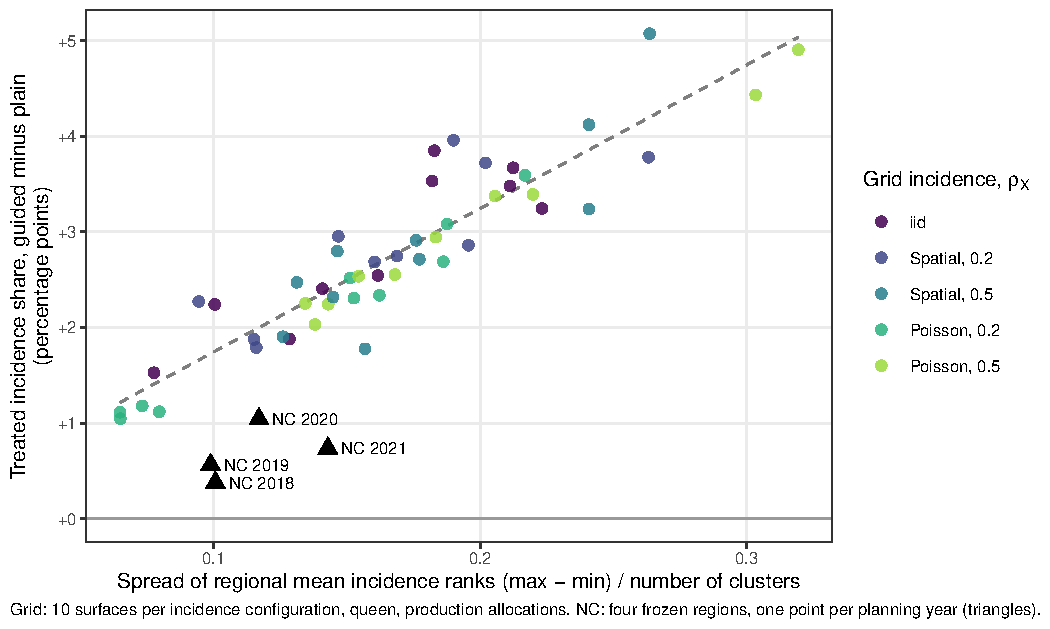
\includegraphics[width=0.9\linewidth]{../figures/fig_spread_vs_gain.pdf}
\caption{Gain in treated incidence share from incidence guidance, Incidence-Guided Saturation minus Saturation Quadrants, against the spread of the regions' mean incidence ranks, (largest minus smallest regional mean rank) divided by the number of clusters. Filled symbols are the 50 grid surfaces (queen, production allocations) by incidence configuration, with a least-squares line fitted to the grid surfaces only. Open triangles are the four fixed NC regions in each planning year, whose spread divides by 58 clusters rather than 100.}
\label{fig:spread-gain}
\end{figure}

\textbf{Formal tests on the NC results.} Friedman tests over the 24 combinations of year, $\rho$ and $\gamma$ rejected equal ranks of the nine strategies in all four combinations of regime and $\beta$ ($\chi^2 = 135.3$, 153.8, 150.7 and 179.8 on 8 degrees of freedom, $p \le 2.3\times10^{-25}$; Nemenyi critical difference 2.45). Under control-only spillover, Saturation Quadrants and Incidence-Guided Saturation had the two best average ranks (1.67 and 1.79 with $\beta = 0$; 1.29 and 1.71 with $\beta = 1$), and SRS ranked seventh with $\beta = 0$ and sixth with $\beta = 1$. Under both-arms spillover with $\beta = 0$, High Incidence Focus ranked first (1.88) and SRS sixth (5.17), with the balancing and saturation designs between them. These tests treat the 24 blocks as independent, although the years share one map and some strategies share their simulations across years, so they describe the consistency of the ordering rather than independent evidence.

\textbf{Unequal numbers of trained professionals.} With $m$ proportional to college population and averaging 25, and ICC $= 0.05$, power fell by 0.097 on average across designs, settings and effect sizes. For $d = 0.3$ under both-arms spillover, the mean power over the nine strategies fell from 0.59 to 0.46 with 20 colleges and from 0.88 to 0.77 with 58. MSE rose by a factor of 1.24 to 1.84 across designs and settings, and no design gained relative to the others.

\textbf{Estimation models.} Every model in the sensitivity analysis has the mean $\mu = \alpha \mathbf{1} + \tau Z + \text{Spill}$ with the proportional spillover covariate of the main analysis, and uses the 58-college queen geography. The spatial lag model of the main analysis is $Y = \rho W Y + \mu + \epsilon$, $\epsilon \sim N(0, \sigma^2 I)$. The CAR model is $Y = \mu + u$, $u \sim N\{0, \sigma^2 (I - \lambda S)^{-1}\}$, where $S$ is the symmetric matrix similar to the row-standardized $W$ \citep{ord_estimation_1975}, fitted by maximum likelihood with the \texttt{spautolm} function of the R package \texttt{spatialreg} \citep{bivand_r_2022}. For the reverse comparison, data were generated as $Y = \mu + L\epsilon$ with $LL^\top = (I - \rho S)^{-1}$ and the same values of $\rho$ as the spatial lag data. These runs used four years, $\rho \in \{0, 0.2, 0.5\}$, $\gamma \in \{0.5, 0.8\}$, both regimes and the nine strategies, with 500 fits per setting.

The Bayesian CAR model \citep{leroux_estimation_2000} is $Y_j = \mu_j + \phi_j + e_j$, $e_j \sim N(0, \nu^2)$, with
\begin{equation*}
\phi_j \mid \phi_{-j} \sim N\left(\frac{\lambda \sum_k a_{jk}\phi_k}{\lambda \sum_k a_{jk} + 1 - \lambda},\; \frac{\sigma_\phi^2}{\lambda \sum_k a_{jk} + 1 - \lambda}\right),
\end{equation*}
where $a_{jk}$ is the binary queen adjacency. We used the defaults of the \texttt{S.CARleroux} function of the R package \texttt{CARBayes} \citep{lee_carbayes_2013}, version 6.1.1: independent $N(0, 10^5)$ priors for the regression coefficients, inverse-gamma(1, 0.01) priors for $\nu^2$ and $\sigma_\phi^2$, and a uniform(0, 1) prior for $\lambda$. Each chain ran 25,000 iterations, of which the first 5,000 were discarded, thinned by 5. At $\rho = 0.5$, where fewer than half the chains converged, we reran the same data with 100,000 iterations, 20,000 discarded and thinning by 20. The Bayesian spatial lag model \citep{lesage_introduction_2009} has the same form as the maximum likelihood model, with the defaults of the \texttt{spBreg\_lag} function of \texttt{spatialreg}, version 1.4.3: a $N(0, 10^{12} I)$ prior for the regression coefficients, the prior $p(\sigma^2) \propto 1/\sigma^2$, a Beta(1.01, 1.01) prior for $\rho$ rescaled to its feasible interval, and 10,000 draws of which the first 2,000 were discarded. Both Bayesian models used four years, $\rho \in \{0, 0.5\}$, $\gamma = 0.8$, both regimes and the nine strategies, with 100 fits per setting (14,400 fits per model), and both were fitted to the same data as the maximum likelihood model. We report the posterior mean of $\tau$ and the 95\% equal-tailed credible interval. A chain was counted as converged when the effective sample size of $\tau$ was at least 400 and the absolute Geweke $z$ statistic \citep{geweke_evaluating_1992} was below 1.96.

With the longer chains, 83.1\% of the Bayesian CAR chains at $\rho = 0.5$ converged, against 46.2\% for the shorter chains, but 12.5\% still had an absolute Geweke $z$ of at least 1.96, against about 5\% expected by chance. Among converged chains, the Bayesian CAR estimate was biased by $+0.14$ under both-arms spillover and $+0.22$ under control-only spillover, with credible-interval coverage of 90.4\% and 87.7\%, against biases of $+0.02$ and $+0.03$ and Wald coverage of 93.5\% and 93.2\% for maximum likelihood on the same data. Of the Bayesian spatial lag chains, 94.9\% converged. The median effective sample size of $\tau$ was 8,000 (minimum 5,897) and 5.1\% had an absolute Geweke $z$ of at least 1.96. Its posterior means correlated 0.999 with the maximum likelihood estimates (mean absolute difference 0.017), its bias was at most 0.04 in absolute value in every combination of $\rho$ and regime, and its credible intervals covered 94.6\% to 95.3\% over all chains (94.5\% to 95.3\% over converged chains). The Spearman correlation of its design ordering with that of maximum likelihood averaged 0.96 to 1.00 across the four combinations of $\rho$ and regime (0.83 in the lowest single block), and the best design agreed in every block. Tables \ref{tab:nc-car} and \ref{tab:nc-bayes} give each strategy's MSE relative to SRS under each model.

\begin{table}[!htb]
\small
\centering
\caption{Mean MSE relative to simple random sampling (SRS) under four combinations of data-generating model and fitted model: spatial lag (SAR) or conditional autoregressive (CAR). 58 colleges, $\beta = 0$, mean over 24 blocks (year $\times$ $\rho$ $\times$ $\gamma$). Below 1 is lower error than SRS.}
\label{tab:nc-car}
% SOURCE: application/results/methods_ext_2026-10/sensitivity_summaries/a6_car_ratio_to_srs.csv (code/24_methods_extension_tables.R)
\begin{tabular}{lcccccccc}
\toprule
& \multicolumn{4}{c}{Both arms} & \multicolumn{4}{c}{Control only} \\
\cmidrule(lr){2-5}\cmidrule(lr){6-9}
Data & SAR & SAR & CAR & CAR & SAR & SAR & CAR & CAR \\
Fit & SAR & CAR & SAR & CAR & SAR & CAR & SAR & CAR \\
\midrule
Checkerboard & 2.88 & 2.83 & 2.93 & 3.09 & 2.99 & 2.64 & 3.01 & 3.00 \\
High Incidence Focus & 1.06 & 1.02 & 1.07 & 1.07 & 1.08 & 1.03 & 1.10 & 1.09 \\
Saturation Quadrants & 1.04 & 1.02 & 1.04 & 1.03 & 0.79 & 0.81 & 0.81 & 0.78 \\
Isolation Buffer & 4.11 & 4.13 & 4.16 & 4.45 & 1.03 & 0.95 & 1.03 & 1.05 \\
$2\times2$ Blocking & 0.98 & 0.99 & 1.00 & 1.02 & 1.21 & 1.17 & 1.22 & 1.22 \\
Balanced Quartiles & 1.04 & 1.05 & 1.04 & 1.06 & 1.03 & 1.00 & 1.03 & 1.02 \\
Balanced Halves & 1.04 & 1.03 & 1.05 & 1.04 & 1.02 & 0.98 & 1.03 & 0.99 \\
Incidence-Guided Saturation & 1.03 & 1.04 & 1.04 & 1.03 & 0.81 & 0.82 & 0.81 & 0.76 \\
Simple Random Sampling & 1.00 & 1.00 & 1.00 & 1.00 & 1.00 & 1.00 & 1.00 & 1.00 \\
\bottomrule
\end{tabular}
\end{table}

\begin{table}[!htb]
\small
\centering
\caption{Mean MSE relative to simple random sampling (SRS) at $\rho = 0.5$ for maximum likelihood (ML), the Bayesian spatial lag model (Bayes SAR) and the Bayesian CAR model with converged chains only (Bayes CAR), all fitted to the same spatial lag data. 58 colleges, $\beta = 0$, $\gamma = 0.8$, mean over the four planning years.}
\label{tab:nc-bayes}
% SOURCE: application/results/methods_ext_2026-10/sensitivity_summaries_v2/a6_bayes_lag_ratio_to_srs.csv (code/24_methods_extension_tables.R)
\begin{tabular}{lcccccc}
\toprule
& \multicolumn{3}{c}{Both arms} & \multicolumn{3}{c}{Control only} \\
\cmidrule(lr){2-4}\cmidrule(lr){5-7}
Design & ML & Bayes SAR & Bayes CAR & ML & Bayes SAR & Bayes CAR \\
\midrule
Checkerboard & 3.14 & 3.18 & 2.90 & 3.16 & 3.16 & 2.31 \\
High Incidence Focus & 0.96 & 0.96 & 0.83 & 1.19 & 1.19 & 1.04 \\
Saturation Quadrants & 1.12 & 1.10 & 1.11 & 0.86 & 0.86 & 1.05 \\
Isolation Buffer & 3.89 & 3.94 & 3.80 & 1.01 & 1.02 & 0.87 \\
$2\times2$ Blocking & 1.14 & 1.14 & 1.11 & 1.48 & 1.48 & 1.34 \\
Balanced Quartiles & 1.00 & 1.00 & 1.05 & 1.10 & 1.10 & 1.15 \\
Balanced Halves & 0.97 & 0.97 & 0.99 & 1.05 & 1.06 & 1.01 \\
Incidence-Guided Saturation & 1.12 & 1.10 & 1.13 & 0.81 & 0.81 & 0.95 \\
Simple Random Sampling & 1.00 & 1.00 & 1.00 & 1.00 & 1.00 & 1.00 \\
\bottomrule
\end{tabular}
\end{table}

\textbf{Spillover form.} Under the binary form, $S(Z) = \gamma\,\mathbf{1}\{\text{any treated queen neighbor}\}$, times $1 - Z$ under control-only spillover. Under the count form, $S(Z) = (\gamma/\bar d) \times$ (number of treated queen neighbors), where $\bar d = 4.93$ is the mean number of queen neighbors, so a college of average degree with every neighbor treated receives $\gamma$, as under the proportional form. Table \ref{tab:nc-forms} compares the three forms. Under the binary form, Isolation Buffer is never identified, because every control has a treated neighbor, and under control-only spillover no strategy was identified in every fit. The saturation designs were identified most often there (in 89.7\% and 91.7\% of fits) and, among identified fits, had MSE 0.70 to 0.71 times that of SRS.

\begin{table}[!htb]
\small
\centering
\caption{Mean MSE relative to simple random sampling (SRS) under three spillover forms, 58 colleges, $\beta = 0$, mean over 16 blocks (year $\times$ $\rho$ $\times$ $\gamma$). n.i.: not identified in every fit (the spillover covariate is aliased with the intercept and treatment in some or all allocations).}
\label{tab:nc-forms}
% SOURCE: application/results/methods_ext_2026-10/sensitivity_summaries/a7_ratio_to_srs.csv, a7_identification.csv (code/24_methods_extension_tables.R)
\begin{tabular}{lcccccc}
\toprule
& \multicolumn{3}{c}{Both arms} & \multicolumn{3}{c}{Control only} \\
\cmidrule(lr){2-4}\cmidrule(lr){5-7}
Design & Proportional & Count & Binary & Proportional & Count & Binary \\
\midrule
Checkerboard & 2.97 & 1.78 & 1.07 & 3.09 & 1.41 & n.i. \\
High Incidence Focus & 0.91 & 0.92 & 0.96 & 1.03 & 1.04 & n.i. \\
Saturation Quadrants & 1.01 & 1.02 & 1.03 & 0.76 & 0.81 & n.i. \\
Isolation Buffer & 3.82 & 3.84 & n.i. & 0.95 & 1.16 & n.i. \\
$2\times2$ Blocking & 1.04 & 1.03 & 1.00 & 1.17 & 1.07 & n.i. \\
Balanced Quartiles & 1.01 & 1.01 & 1.00 & 0.99 & 0.99 & n.i. \\
Balanced Halves & 1.02 & 1.02 & 1.02 & 0.98 & 0.99 & n.i. \\
Incidence-Guided Saturation & 1.01 & 1.03 & 1.04 & 0.75 & 0.79 & n.i. \\
Simple Random Sampling & 1.00 & 1.00 & 1.00 & 1.00 & 1.00 & n.i. \\
\bottomrule
\end{tabular}
\end{table}

\FloatBarrier
\bibliographystyle{unsrtnat}
\bibliography{SpatialCRT_IncidenceDesign}
\end{document}
